%%%%%%%%%%%%%%%%%%%%%%%%
%% Sample use of the infthesis class to prepare a thesis. This can be used as 
%% a template to produce your own thesis.
%%
%% The title, abstract and so on are taken from Martin Reddy's csthesis class
%% documentation.
%%
%% MEF, October 2002
%%%%%%%%%%%%%%%%%%%%%%%%

%%%%
%% Load the class. Put any options that you want here (see the documentation
%% for the list of options). The following are samples for each type of
%% thesis:
%%
%% Note: you can also specify any of the following options:
%%  logo: put a University of Edinburgh logo onto the title page
%%  frontabs: put the abstract onto the title page
%%  deptreport: produce a title page that fits into a Computer Science
%%      departmental cover [not sure if this actually works]
%%  singlespacing, fullspacing, doublespacing: choose line spacing
%%  oneside, twoside: specify a one-sided or two-sided thesis
%%  10pt, 11pt, 12pt: choose a font size
%%  centrechapter, leftchapter, rightchapter: alignment of chapter headings
%%  sansheadings, normalheadings: headings and captions in sans-serif
%%      (default) or in the same font as the rest of the thesis
%%  [no]listsintoc: put list of figures/tables in table of contents (default:
%%      not)
%%  romanprepages, plainprepages: number the preliminary pages with Roman
%%      numerals (default) or consecutively with the rest of the thesis
%%  parskip: don't indent paragraphs, put a blank line between instead
%%  abbrevs: define a list of useful abbreviations (see documentation)
%%  draft: produce a single-spaced, double-sided thesis with narrow margins
%%
%% For a PhD thesis -- you must also specify a research institute:
\documentclass[phd,icsa,twoside]{infthesis}

%% For an MPhil thesis -- also needs an institute
% \documentclass[mphil,ianc]{infthesis}

%% MSc by Research, which also needs an institute
% \documentclass[mscres,irr]{infthesis}

%% Taught MSc -- specify a particular degree instead. If none is specified,
%% "MSc in Informatics" is used.
% \documentclass[msc,cogsci]{infthesis}
% \documentclass[msc]{infthesis}  % for the MSc in Informatics

%% Master of Informatics (5 year degree)
% \documentclass[minf]{infthesis}

%% Undergraduate project -- specify the degree course and project type
%% separately
% \documentclass[bsc]{infthesis}
% \course{Artificial Intelligence and Psychology}
% \project{Fourth Year Project Report}

%% Put any \usepackage commands you want to use right here; the following is 
%% an example:
\usepackage[section]{placeins}
\usepackage{pdflscape}
\usepackage{url}
\usepackage{amsmath}
\usepackage{graphicx}
\usepackage{subfig}
\usepackage{multicol}
\usepackage{lipsum}
\usepackage{siunitx}
\usepackage{booktabs}
\usepackage[table]{xcolor}
\usepackage{booktabs}
\usepackage{xspace}
\usepackage{balance}
\usepackage{listings}
\usepackage{lstlinebgrd}
\usepackage[]{algorithm2e} 
\usepackage{algpseudocode}
\usepackage{rotating}
\usepackage{booktabs} % For formal tables
\usepackage{textcomp}
\definecolor{listinggray}{gray}{0.9}
\definecolor{lbcolor}{rgb}{0.9,0.9,0.9}
\usepackage{subfig}
\usepackage{verbatim}
\usepackage[titletoc]{appendix}
\usepackage[normalem]{ulem}
\usepackage{amsmath}
\usepackage{mathtools}
\usepackage{xspace} 
\usepackage{float}
\DeclarePairedDelimiter\ceil{\lceil}{\rceil}
\DeclarePairedDelimiter\floor{\lfloor}{\rfloor}
\usepackage{todonotes}
\SetKwComment{Comment}{$\triangleright$\ }{}
\renewcommand{\theparagraph}{\arabic{paragraph}}
\newcommand{\ie}{i.\,e.\xspace}
\newcommand{\eg}{e.\,g.\xspace}
\newcommand{\bench}[1]{\textit{#1}\xspace}
\usepackage[labelfont=bf]{caption}
%% Information about the title, etc.
\title{From Software to Hardware: Making Dynamic Multicore Processors Practical}
\author{Paul-Jules Micolet}

%% If the year of submission is not the current year, uncomment this line and 
%% specify it here:
% \submityear{1785}

%% Optionally, specify the graduation month and year:
% \graduationdate{February 1786}

%% Specify the abstract here.
\abstract{%
    This doctoral thesis will present the results of my work into the
    reanimation of lifeless human tissues.
}

%% Now we start with the actual document.
\begin{document}

%% First, the preliminary pages
\begin{preliminary}

%% This creates the title page
\maketitle

%% Acknowledgements
\begin{acknowledgements}

Many thanks to my mummy for the numerous packed lunches; and of course to
Igor, my faithful lab assistant.
\end{acknowledgements}

%% Next we need to have the declaration.
\standarddeclaration

%% Finally, a dedication (this is optional -- uncomment the following line if
%% you want one).
% \dedication{To my mummy.}

%% Create the table of contents
\tableofcontents

%% If you want a list of figures or tables, uncomment the appropriate line(s)
% \listoffigures
% \listoftables

\end{preliminary}

%%%%%%%%
%% Include your chapter files here. See the sample chapter file for the basic
%% format.
\chapter{Introduction}
%From StreamIt paper
Multicore processors are now common in all computing systems ranging from mobile devices to data centers.
As advances in single threaded performance have slowed, multicore processors have offered a way to use the increasing numbers of transistors available.
However, designing processors that scale to a large number of cores is difficult and a shift towards tiled architecture seems inevitable.
A tiled architecture such as Tilera~\cite{bell2008tile} or Raw~\cite{waingold1997raw} is composed of smaller simpler cores that are placed on a regular grid.
This improves hardware scalability and enables multi-threaded applications to exploit the large core count.

% Tiled architecture problem: cores too weak => need reconfiguration
However, workloads that require high single threaded performance are penalized by the simple nature of each core~\cite{eyerman2010amdahl}.
One solution to this problem is heterogeneous multicores which utilize cores with different levels of power and performance.
Although heterogeneous multicores are common place in mobile devices, they have little reconfiguration or adaptive capabilities (\eg only two type of cores available for ARM big.LITTLE).
Dynamic multicore processors offer a solution to this problem by allowing cores to compose (or fuse) together~\cite{ipek2007CoreFusion} into larger logical cores to accelerate single threads.
This produces ``on-demand'' heterogeneity where cores are grouped to adapt to the workload's demand.

\section{The Problem}

\paragraph*{Dynamic multicore processor reconfiguration}
Whilst there exists a multitude of proposed dynamic multicore processor architectures ~\cite{MittalSurv2016} work on understanding when to compose cores, or what type of programs can benefit the most out of core composition is scarce.
A 16 core DMP for example has over 15,000 configurations when executing multi-threaded programs, making exhaustive search of the space impractical.
Therefore, without some method of automating the reconfiguration of the processor the programmer must have intimate knowledge of both the architecture and the programs that will execute on them.

Previous work on determining how many cores must be composed for a given program at runtime or ahead of time focus on using profiling information~\cite{pricopiSchedCoreComp2014} or heuristics based on observations~\cite{gulati2008multitaskingdmc}.
They consider core composition to be a \textit{black box}: instead of trying to understand what features of a program lead to good performance, they will instead evaluate it on different core composition sizes and determine the best one.
This approach makes DMPs less practical as it increases the amount of work required to ensure that workloads benefit from core composition.

If the system could determine the correct configuration of the processor by analysing the source-code or assembly of a program, then this would make the process of getting the best performance lightweight.
This would allow programers to modify their programs without having to extensively re-profile their applications, making dynamic multicore processors more approachable.

\paragraph*{Benefiting from core composition}
Not all applications will benefit from executing on a core composition, which can reduce the attractiveness of implementing the feature in a processor.
The lack of performance may be due to the fact that the programs were not initially designed to be executed on a system that supports core composition.
Programmers may have to re-design their code to ensure that a program that currently does not perform any better could not be re-written to benefit from the new hardware.

However, there exists no information as to what optimisations may help improve the performance of applications on a dynamic multicore processor.
Furthermore, a programmer may not necessarily have access to a compiler that provides passes that are targetted towards such systems.
In this case, it is important to explore source-level optimisations and study how they can help increase the performance of programs on core composition.
By underlining which optimisations will lead to performance improvements, this encourages the ease-of-use of dynamic multicore processors.

\paragraph*{Core composition mechanisms} 
Finally, as the concept of dynamic multicore processors is still relatively new compared to other processor designs, the currently proposed techniques may not be enough to maximise performance.
For example, core composition exploits instruction level parallelism by executing a single thread through the use of aggressive speculation.
Yet, there the architectures proposed in research do not discuss how data-dependencies, that often occur when many instructions are executing in parallel, can be resolved quickly.
This means that dynamic multicore processors will not improve performance to the fullest of their capacities.

It is therefore important to critically analyse where the current bottlenecks of core composition are from a hardware perspective.
By proposing solutions to these bottlenecks, core composition can become more effective at improving the performance of programs.
Modifications to the hardware can even help dynamic multicore processors become more adaptable to new types of programs, once again making them more practical.


\section{Contributions}
This thesis tackles the three problems that were previously described through the use of different techniques.

In order to provide a more general solution towards automating the reconfiguration of a DMP, both at runtime and ahead of time, a set of machine learning models that are able to automatically make configuration decisions based on features of the software are proposed.
This thesis presents a design methodology for generating these models that use either program features that can be extracted at the source level or features that can be used at runtime, to determine when and how to configure the cores.
These models are not influenced by hand-picked heuresitics, but instead are generated by exploring how different configurations affect performance, and analysing how different programs' performance is improved by core composition.
By using machine learning, the processor can automatically be reconfigured ahead of time to improve the performance of multithreaded applications, or at runtime to reduce energy consumption.

This thesis also provides an analysis of how different features of the source-code affect the speedup that can be gained from core composition.
This is achieved by exploring a set of source-level optimisations and studying the generated code of applications that perform both well and poorly.
The analysis provides insights on when core composition should be used, and how programs may be modified to get more performance.

Finally, the current shortcomings of core composition are brought forward.
The two main features of the hardware that are analysed are how instructions are fetched when cores are composed and how data-dependencies affect the performance of large core compositions.
By providing a new fetching scheme, and implementing a value predictor which can speculate the results of instructions, this thesis shows that the mechanisms of core composition can be improved.


\section{Structure}
The overall aim of this thesis is to provide methods of making DMPs more practical, from automated reconfiguration to new hardware that improves the overall performance of the DMP.
The structure of the thesis is as follows:

\textbf{Chapter ~\ref{chp:Background}} provides information on the different topics approached throughout this thesis. The topics involve the reconfiguration mechanisms of DMPs, the EDGE architecture, how value prediction works and the different machine learning techniques used throughout this thesis.

\textbf{Chapter ~\ref{chp:rw}} presents the related work. This covers previously proposed DMP processors and the different offline and online reconfiguration schemes that are suggested. 
This is followed by a discussion of work done on compiler optimisations for EDGE, the different hardware techniques that improve energy efficiency, other proposed value predictors and different types of speculative hardware.

\textbf{Chapter ~\ref{chp:setup}} covers the setup of the cycle-accurate simulator used throughout this thesis.

\textbf{Chapter ~\ref{chp:streamit}} explores how a dynamic multicore processor can be configured to improve the performance of multi-threaded streaming applications.
The chapter demonstrates that a mix of core composition and multithreading is requried to get the best speedup for these applications.
A machine learning model is then trained to determine a good configuration of the processor based on source-code information derived from the application.
This chapter is based on the work previously published in ~\cite{micolet2016dmpstream}.

\textbf{Chapter ~\ref{chp:cases}} uses dynamic reconfiguration to reduce energy consumption whilst maintaining the same performance as the optimal static ahead of time configuration.
The chapter first covers some of the factors that affect the performance of core compositions, such as branch prediction accuracy requirements folowed by a study of how dynamically adapting the processor at runtime can reduce energy consumption.
A machine learning model that can determine the correct size of a core composition at runtime, based on the types of instruction being executed is then designed.
The chapter is based on the work previously published in ~\cite{micolet2017cases}.

\textbf{Chapter ~\ref{chp:hardchanges}} presents modifications to the hardware that allow larger core compositions to perform better in the average situation.
The modifications involve a new fetching mechanism that ensures each core can fetch blocks independently and in a round robin fashion and the use of value prediction to minimise stress on the network on chip and reduce the effect of data dependencies between cores.

\textbf{Chapter ~\ref{chp:conclusion}} finally concludes this thesis by summarising the contributions, providing critical analysis and presenting future work in the field of dynamic multicore processors.
\chapter{Background}
This chapter covers the different topics that are present in this thesis.
The background starts by briefly covering Chip Multicore Processors and Heterogeneous Chip Multicore Processors to motivate the existence of Dynamic Multicore Processors.
Then the core-fusion technique, which is the main mechanism brought forward by Dynamic Multicore Processors is described in detail.
This is followed by a description of the EDGE instruction set architecture which is used in the Dynamic Multicore Processor described in this thesis.
Finally, streaming programming languages, which are used in Chapter~ref{}, are explained.

\section{Chip Multicore Processors}

\begin{figure}[t]
 \center
 \includegraphics[width=1\textwidth]{background/graphics/i7intel.jpg}
 \caption{Intel Core i7 processor internal die photograph taken from intel whitepaper}\label{fig:i7}
\end{figure}
 
Chip Multicore Processors (CMPs) have become ubiquitous due to the difficulty in scaling single core performance.
In a CMP, multiple processor cores are put on a single package as can be seen in Figure~\ref{fig:i7}.
The most common CMP uses homogeneous cores as they reduce the design complexity both from a hardware and software perspective~\cite{}.
Unlike single core systems, the performance improvement in CMPs come from running multiple tasks in parallel.
These tasks can either be different programs or multiple threads from the same program running on the multiple cores.
By defining speedup \textit{S} to be the original execution time of the program over the new execution time with \textit{n} processors and \textit{f} representing the fraction of the program which can be parallelised; Amdahl's Law states

\begin{equation}
S = \frac{1}{(1-f) + \frac{f}{n}}
\end{equation}\label{amdlaw}

thus, given an infinite number of processor cores~\cite{ekhout2010amdalh}

\begin{equation}
\lim_{n\to\infty} S = \frac{1}{(1-f)}
\end{equation}

This second equation demonstrates how, given any program, the speedup obtained by using a CMP will be limited to the fraction \textit{f} of parallel code found in the program itself.
As all the processor cores are homogeneous this will cause serial bottlenecks to severely reduce the potential speedup as no core is adapted to speedup such regions.
This implication has pushed research into finding ways of parallelising code to its fullest~\cite{}, however this may not always be possible~\cite{}.
Thus whilst CMPs have become a mainstain in processor design, the homogeneous model has its limits.

\section{Heterogeneous Chip Multicore Processors}

\begin{figure}[t]
 \center
 \includegraphics[width=1\textwidth]{background/graphics/biglittle.png}
 \caption{Example of a heterogeneous multicore processor proposed by ARM (big.LITTLE)}\label{fig:blarm}
\end{figure}

Unlike CMPs, Heterogeneous Chip Multicore Processors (HCMPs) or Asymmetrical Chip Multicore Processors (ACMPs) bring a variety of cores onto a single package.
This may come in different forms, such as having multiple instruction set architectures on the same system on chip (MPSoCs)~\cite{venkatharnessingISA,hipstr}, or same ISA different size cores on an SoC~\cite{bigLittle}.
For example, Figure~\ref{fig:blarm} shows a schemata for ARM's big.LITTLE HCMP, where a high-performance Cortex-A15 is paired with a simpler, power efficient Cortex-A7.
The two cores are connected via a cache coherent interconnect which provides data coherence at the bus-level, allowing the cores to make reads to its neighbor.
Software is then run on one of the cores depending on a profile; if the user requires performance over energy, then the Cortex-A15 will be chosen, however if energy/power efficiency is required then the Cortex-A7 will be chosen.

This small example already demonstrates an advantage of HCMPs; unlike CMPs, the variety of cores on an HCMP provide a flexibility to the hardware.
This can be used for different purposes, such as security~\cite{hipstr}, energy/power savings~\cite{venkatharnessingISA} and speeding up applications~\cite{venkatharnessingISA}.
In their 2014 paper, Venkat et al.~\cite{venkatharnessingISA} demonstrate that a multi-ISA HCMP can improve performance by up to 1.4x and achieve energy savings of up to 40\% compared to a CMP on a peak-power budget of 40W.
They motivate the idea that HCMPs with heterogeneous ISAs even improve over the performance of single-ISA HCMPs with speedups around 15\% and energy savings of 21.5\%.

However, whilst the hardware diversity in HCMPs is an advantage compared to CMPs, it also increases programming complexity.
For example, Gupta et al. in ~\cite{dypo} show that a single-ISA octa-core big.LITTLE architecture can have 20 CPU cores, combined with the ability to dynamically modify the voltage, this leads to 4000 different configurations.
This highly increases the complexity of obtaining the correct settings for different programs.
MPSoCs also face a similar issue as having more than a single ISA not only adds design challenges, but program migration between different cores may in fact deteriorate performance~\cite{asplos2012}.

\section{Dynamic Multicore Processors}

% This section explains what a dynamic multicore is

In both CMPs and HCMPs, once the chip is fabricated the design cannot be modified, meaning that many of the trade-offs between power, performance and area cannot be changed after production.
Dynamic Multicore Processors (DMPs) attempt to bridge the gap between the two previous designs by allowing the execution substrate to adapt dynamically at runtime.
Mitall's survey ~\cite{MittalSurv2016} defines three types of modifiable resources: the core count~\cite{ipek2007CoreFusion}, number of resources that each core has~\cite{Homayoun3DPooling2012} and microarchitectural features~\cite{fallinhetblock2014,BauerRSE08,tavanaElastic}.

\subsection{Core Fusion Dynamic Multicore Processors}

\begin{figure}[t]
    \centering
    \includegraphics[width=.7\textwidth]{streamit-paper/graphics/dmcgraph.pdf}
    \caption{High-level view of a dynamic multicore processor that can modify its core count.}
    \label{fig:dynmulticore}
\end{figure}

A DMP that modifies core count is composed of homogeneous cores with a reconfigurable fabric.
Physical cores can function either on their own or as a group of physical cores; this is called a Logical Core (LC).
Throughout this thesis, the term core-fusion will be used to define the mechanism of cores creating an LC.
A logical core will fetch instructions from a single source and execute them accross all the physical cores that compose the LC.
Cores can fuse dynamically and create a logical core of any sizes.
For example in Figure~\ref{fig:dynmulticore}, the DMP fuses cores into 3 LCs of sizes 1, 8 and 6 physical cores.
The exact mechanism of core-fusion are described later on in Section~\ref{sec}.

The advantage of a core-fusion DMP over the traditional CMP or HCMP is the ability to reconfigure the processor dynamically to better match the tasks at hand.
For example, large sequential sections of code with high Instruction Level Parallelism (ILP) can be accelerated on a logical core that mimics a wide superscalar processor.
On parallel workloads the DMP can be reconfigured by de-composing the logical cores as seen in Figure~\ref{fig:dynmulticore} to match the Thread Level Parallelism (TLP).

%More here
\subsection{Resource Sharing Dynamic Multicore Processors}
A more fine-grained reconfiguration can be found in resource-sharing DMPs.
There exist different models for resource sharing DMPs.
For example the WiDGET DMP by Watanabe et al.~\cite{watanabe}, cores are built out of Instruction Engine front-ends which function similarly to Out of Order (OoO) cores' front and back ends.
They then are connected to Execution Units which they can choose to use.
Each core in the WiDGET DMP also have access to their neighbors Execution Units, allowing for more variation.
Another example of resource sharing can be found in Rodrigues et al.'s work~\cite{} where a core can use resources such as Arithmetic Logic Units (ALUs) from other cores.

%More here
\subsection{Microarchitectural Reconfigurable Dynamic Multicore Processors}
A final example is a DMP which can reconfigure microarchitectural features to better fit the current application.
Fallin et al.~\cite{fallin} observe that serial code can exhibit phases that fit different microarchitectural features.
According to them, these phases may only been in the ten to hundred thousands instructions long.
These DMPs can therefore modify microarchitecural features, such as in-order or out-of-order execution, to best match the current phase of a program.

\begin{figure}[t]
    \centering
    \includegraphics[width=1\textwidth]{background/graphics/EDGE_3.pdf}
    \caption{High-level view of the EDGE ISA flow.}
    \label{fig:EdgeHigh}
\end{figure}

\section{EDGE Instruction Set Architecture} 
The Explicit Data Graph Execution~\cite{burger04edge} (EDGE) instruction set architecture (ISA) is a data-flow based ISA.
Figure~\ref{fig:EdgeHigh} shows a high-level overview of how EDGE differs from a traditional instruction set architecture.
The EDGE compiler has a first pass which generates instructions from the original source code.
Blocks are then generated from the basic-blocks found in the code generation pass.

%what I'm trying to say here is that registers are used only for outer communication, in a block instructions are 
Unlike traditional ISAs, blocks do not communicate via registers, but rather the output targets of instructions are encoded to instruction inputs~\cite{smith2006edge}.
Loads and stores in each EDGE block are assigned unique identifiers which are used resolve load-store dependencies.
Thus, the EDGE ISAs encode dependencies between instructions at the ISA level, registers are only used for inter-communication between blocks.
An EDGE block also contains a header that will inform the hardware about the number of stores and register writes contained in the block~\cite{e2paper}, this is used to facilitate committing blocks.

EDGE blocks also have a set of restrictions to satisfy correctness.
If a block does not meet these requirements, it may need to be broken down into smaller blocks.
These restrictions are:

\begin{itemize}
\item Block Size: an EDGE block may be between 4 to 128 instructions.
\item Load/Store: an EDGE block may have at most 32 load/store instructions.
\item Entry/Exit: an EDGE block may have a single exit but may have multiple exits.
\end{itemize}

To increase the average size of EDGE blocks, multiple blocks can be combined together to form one large block called a hyperblock.
This is achieved through the use of instruction predication.
For example given an if/else statement, the compiler can generate a single block, predicating all instructions of the else statement.
As the compiler needs to declare the number of stores and register writes in the block header, extra instructions may need to be generated to ensure the block always executes the same amount of stores.

Overall, the EDGE ISA enables the architecture to dispatch blocks speculatively, with low overhead~\cite{putnam2010e2,kim2007tflex}, therefore, increasing exploitation of ILP.

\section{EDGE Processor}

\subsection{Core Lanes}
 \begin{figure}[t]
 \center
 \includegraphics[width=1\textwidth]{background/graphics/e2segment.png}
 \caption{Example of a four lane core on an EDGE processor taken from~\cite{e2smith}.}\label{fig:e2segment}
 \end{figure}
 
EDGE instruction blocks can be up to 128 instructions long, however this often isn't the case.
To maximize core-utilisation, each core on an EDGE Processor is segmented into a set number of lanes which can each fetch and decode their own blocks.
A lane is able to fetch a block of maximum size

\begin{equation}
\frac{128}{NumberOfLanes}
\end{equation}

For example, a four lane core as seen in Figure~\ref{fig:e2segment} can have up to four blocks of 32 instructions.
Fetching blocks larger than 32 instructions will fill up more than one lane.
Lanes allow EDGE cores to be more flexible to block size variability.

\subsection{Core Fusion}
 \begin{figure}[t]
 \center
 \includegraphics[width=1\textwidth]{cases-paper/graphics/background/proc_test.pdf}
 \caption{Core Fusion Mechanisms for our EDGE-based architecture.}\label{fig:dmp}
 \end{figure}
 
Core Fusion is achieved by fusing a set of \textit{physical} cores to create larger \textit{logical} cores.
This does not modify the physical structure of the chip, instead it provides a unified view of a group of physical cores to the software.
In the processor used throughout the thesis, the micro-architecture is distributed: register files, Load Store Queues (LSQs), L1 caches and ALUs all look like nodes on a network.
This means that when cores fuse together, this is similar to adding an extra node to the network.
Fusion is a dynamic modification and may occur during the execution of a program to better fit the workload.
Unlike traditional CMPs, fused cores will operate on the same thread and attempt to extract Instruction Level Parallelism (ILP) rather than Thread Level Parallelism (TLP)~\cite{micolet2016dmpstream,pricopi2012bahurupi}.

Figure~\ref{fig:dmp} shows the different stages and mechanisms of core fusion for a four core system.
When creating a new core fusion a master core informs all other cores about the fusion and sends the predicted next block address to the next available fused core.
When we start a new thread on a fused core the OS and runtime write the new core mapping to a system register.
The hardware then flushes these cores if they are not idle and sets the PC of the first block of that thread on one core in the logical processor and starts executing.
When a core mispredicts a branch in a fusion, it informs the other cores which flush any younger blocks.
When un-fusing, the master core informs the other cores, which then commit or flush their blocks and power down while the master core continues to fetch and execute blocks from the thread.
The extra hardware required to support dynamic reconfiguration is very minimal~\cite{kim2007tflex} since most of the machinery already in place can be reused such as the cache coherence protocol when fusing and un-fusing the cores.

When a logical core fetches multiple blocks, it may execute them out of order.
However memory instructions and instructions that modify registers pass through the LSQ and register-file and are executed in order.
This ensures that blocks operate on memory in a consistent fashion.
In case of a memory violation caused by undetected dependencies a flush of all blocks younger than the violator, including the violating block, is performed.

%Fusing cores is therefore a lightweight process.
%We estimate that switching the size of the logical-core (LC) results in a delay of 100 cycles on average.
%The actual time varies based on the time it takes the cache coherence protocol to move the data around the memory system.
%Section~\ref{sec:reconfoverhead} discusses in more details how latency affects energy efficiency and shows that dynamic core fusion is still highly beneficial even when considering overheads of 1,000 cycles.

\section{Streaming Programming Languages}

% % This section should explain what steaming programming is (remove all the details about each language)
% General purpose programming languages often propose very little support for programs that handle with a continuous flow of data.
% This results in having to design a set of complicated for loops to manage the streams of data.
% Having to deal with different rates of incoming and outcoming data also increases the complexity of writing these applications using a standard language.

Streaming programming languages are a branch of dataflow programming that focus on applications that deal with a constant stream of data.
These applications, such as audio or video decoding can be commonly found in mobile devices.
Unlike conventional programming languages such as C++, these languages abstract the concept of incoming and outgoing data to permit the programmer to focus on how the data should be treated.
Programs are described as directed graphs where nodes are functions and their edges represent their input and output streams. 
These languages offer primitives to describe such a graph~\cite{theis2002streamit} which expose parallelizable and serial sections of the application directly to the compiler. 
Rates of incoming and outcoming data can also be defined to facilitate load balancing optimizations~\cite{chen2005rawstream}.

Features of streaming programming languages make them an ideal language for targeting multicore processors.
The explicit data communication between the different tasks in the program, the ability to estimate the amount of work performed in each task and information about data rates between tasks allows the compiler to easily generate a multi-threaded application that can run on a dynamic multicore processor.
However, the main challenge consists of deciding how to map the different tasks onto threads and how to allocate the right amount of resources to maximize performance.

\section{Machine-learning guided optimisations}
\label{chp:bg}
\chapter{Related Work}
This chapter covers the related work relevant to this thesis.
The topics covered are:
\begin{itemize}
\item The different dynamic multicore processors using core composition proposed in recent research.
\vspace{-1em}
\item Work on determining core composition sizes.
\vspace{-1em}
\item Research on different hardware techniques for saving energy.
\vspace{-1em}
\item Work on streaming programming languages.
\vspace{-1em}
\item Work on machine learning guided optimisations in both hardware and software.
\vspace{-1em}
\item Current research in value prediction.
\end{itemize}

\section{Reconfigurable Processors}

This section covers work on both dynamic multicore processors (DMP) and processors that can reconfigure their microarchitectures.

\subsection{Core composition}
The idea of composing physical cores was first introduced by Ipek et al. in CoreFusion~\cite{ipek2007CoreFusion}.
CoreFusion employs a traditional architecture with 2 issue out of order cores.
When cores are fused, they collectively fetch from the same thread, whenever an instruction cache miss is issued, an eight word block is delivered and distributed across all of the cores' caches.
Fetches are aligned with the core responsible for the 2 oldest instructions.
In the original paper, an 4 core composition obtains a 1.3x speedup on SPECINT and a 1.5x speedup on SPECFP over a 2 issue core.
 
The Bahurupi~\cite{pricopi2012bahurupi} polymorphic heterogenous multicore architecture proposed by Pricopi et al. introduces a sentinel instruction which informs the hardware about the \textit{live-in} and \textit{live-out} registers of a basic block.
Baharupi uses the SimpleScalar ISA~\cite{burger1997simplescalar}, and the compiler adds this instruction to the top of every basic block, splitting the program up into blocks similarly to EDGE.
They show that, on average this introduces a 24\% code size increase for SPEC integer applications, 15\% for SPEC floating point and 19\% for Mediabench~\cite{mediabench} and MiBench~\cite{mibench} benchmark suites.

Another important piece of information contained in this instruction is the size of a block.
Cores in a composition fetch basic blocks in a similar fashion to the one described in Chapter~\ref{chp:Background} Section~\ref{chp:Background:sec:EDGE}.
However, cores must execute global register renaming in the sequential order of blocks.
To ensure sequential renaming, a Global Program Counter (GPC) is introduced, and each core in the composition must lock the GPC before fetching a block and doing the renaming; this makes Baharupi less efficient at fetching blocks than EDGE.
Using a 4 core composition they report a performance improvement of 2x on SPECINT,3x on SPECFP and 4x on Mibench/Mediabench compared to a 2 issue core. 

TFlex~\cite{kim2007tflex} proposed by Kim et al. is an EDGE processor that also deploys core composition.
The mechanism is similar to the one described in Chapter~\ref{chp:Background} Section~\ref{chp:Background:sec:EDGE}.
They motivate that EDGE simplifies distributing instructions accross cores as EDGE itself is designed for distributed microarchitectures.
Unlike the model used throughout this thesis, a block's instructions can be distributed amongst the cores in the composition, with one of the cores being the block owner.
As each core can be responsible for a single block, the total number of blocks in flight is equal to the number of cores in the composition.
In their work~\cite{kim2007tflex} Kim et al. show that a 32 core composition can outperform a single TFlex core by 3x on a set of EEMBC benchmarks and SPEC2000 microbenchmarks.

Finally, the E2 processor is another EDGE based processor that can compose its cores~\cite{putnam2010e2}.
Unlike TFlex, when cores are fused in the E2 processor, each core is responsible for the blocks they fetch.
E2 introduces the concept of segmenting the instruction window into lanes, allowing cores to fetch multiple blocks.
The processor explored throughout this thesis is based on the E2 processor.

\subsection{Reconfigurable microarchitectures}
ElasticCore~\cite{tavanaElastic} proposes a morphable core that uses dynamic voltage and frequency scaling (DVFS) and microarchitectural modifications such as instruction bandwidth and capacity to adapt the processor to current needs.
This is similar to the work proposed by Dubach et al. in ~\cite{dubach13dynamic} where microarchitectural features can be modified for better performance or energy efficiency.
They provide extensive analysis of SPEC 2000 benchmarks and demonstrate that machine learning and dynamic adaptation can double the energy/performance efficiency compared to a static configuration.

MorphCore~\cite{khubaibMorphCore2012} focuses on reconfiguring a core for thread level parallelism.
It switches between out-of-order (OoO) when running single threaded applications and an in-order core optimised for simultaneous multi threading (SMT) workloads.
This provides an opposite solution to our DMP: providing a large core made for ILP that can be modified to better fit TLP workloads.
MorphCore outperform a 2-Way SMT OoO core by 10\% whilst being 22\% more efficient.


\section{Automated reconfiguration for DMPS}

Very little work exists on determining the size of a core composition given an application, or when the composition must change.
In Ipek et al's. original work on CoreFusion~\cite{ipek2007CoreFusion} they introduce the \textit{FUSE}/\textit{SPLIT} instructions that allow for dynamic reconfiguration.
However, their eight core system only has two possible configurations: either each core is executes on their own or they are fused into groups of four cores; no details as to when to compose cores is discussed.
This is the same for the original proposal for TFlex~\cite{kim2007tflex}, where 5 different configurations are explored (2, 4, 8, 16 and 32 composed cores), but does not provide any insight as to how to determine the composition size automatically.

In the work of Pricopi et al.~\cite{pricopiSchedCoreComp2014}, they show how dynamic reconfiguration is beneficial when it comes to scheduling multiple tasks.
However, they do not discuss any method of automatically deciding the optimal configuration beyond a 4 core composition.
In their work they use speedup functions determined from profile executions of applications to determine how to schedule tasks.
This means that whenever an application is modified, it must be re-analysed to benefit from dynamic composition.
They do not discuss what software characteristics help determine when to reconfigure the cores, or how to optimise software.

Gulati et al. propose an offline and online scheduling algorithms for Tflex \cite{tflexmultitask}. 
This work focuses on maximising speedup for a set of workloads in a multi-tasking environment.
The offline model uses profiling data to make decisions whereas the online model measures the current performance of a task being exected and switches the size of the composition based on a threshold.
In their results they show that the offline profiling tool outperforms the online algorithm.
As the threshold is set ahead of time, the online model is not able to fully utilise the system when applications do not meet the required threshold.
Overall they demonstrate that a DMP that can adapt to workloads can result in faster response times than a tradition CMP, between 21\% to 13 times faster.

In~\cite{santos2013nocdmc} they use information provided by the application to determine how to reconfigure some components of the processor.
This initial information then assists the rest of the reconfiguration, this process still requires input from the programmer though.

\section{Hardware techniques for power and energy efficiency}

This section covers different hardware techniques used for energy efficiency that do not depend on core composition.

\subsection{Dynamic Voltage and Frequency Scaling}
Dynamic Voltage and Frequency scaling (DVFS) is a method of modifying the power and energy consumption~\cite{paganiEECHM2017} by modifying the voltage or the clock rate of the processor.
Often times, DVFS is used to reduce energy or power consumption in phases of low performance.

Herbert et al in ~\cite{herbertDVFS07} demonstrate that DVFS can be used to reduce $energy/throughput^2$ on a 16 chip multicore processor (CMP) by 39\% on a set of multithreaded workloads.
They argue that on a CMP, DVFS does not need to be on a per-core basis, as fine-grained DVFS does not improve $energy/throughput^2$ by much compared to coarse grained DVFS.

Vega et al. in ~\cite{vega2013crank} underline that whilst DVFS is an effective way of reducing power and energy consumption, the fact that it is decoupled from other techniques such as per core power-gating (PCPG) reduces the overall benefits.
They suggest an online algorithm at the OS level that collects data from performance counters and makes multiple decisions based on the data gathered.
%write more
%However this approach is orthogonal to DMPs~\cite{sibi2014}, whilst both techniques (DVFS and core composition) adapt to programs phases, DMPs can also be used to speed up the execution of programs.

\subsection{Heterogeneous Chip Multicore Processors}
ARM big.LITTLE~\cite{} is an example of a heterogeneous chip multicore processor (HCMP) that provides two different types of cores to allow the programmer to choose between energy efficiency and performance.
A program can be migrated from one core to another depending on the requirements, however this comes at the cost of a very high migration overhead, over 10,000 cycles~\cite{}.
However Gutpa et al. show that by selecting the correct core configuration at runtime this can lead to an energy reduction of up to 46\%

%More on HAQUE
Haque et al. show that an HCMP is able to reduce energy consumption and improve throughput for applications with high-percentile latencies~\cite{tailAMP2017}.
They highlight that service provides receive requests of different lengths of computation.
By successfuly scheduling the different lengths to the correct cores in an HCMP, they can reduce the energy consumption of short requests by a factor of 50\% compared to DVFS.

\section{Speculative Execution}
Core composition is able to improve performance of applications by executing many instructions speculatively from the same thread.
This section covers work on speculative parallelism, where performance improvements are obtained by speculatively executing mutliple tasks in parallel, rather than through deep branch prediction.

\paragraph*{Software level}
The idea of speculatively extracting parallelism at runtime was first introduced by Rauchwerger et al. in~\cite{runtimeSpec}.
They underlined that compile-time analysis of single-threaded programs does not allow for the complete detection of parallel sections, and must be completented by runtime analysis.
They proposed a framework for parallelising loops at runtime: instead of detecting if the loop is parallelisable or not, the loop is speculatively executed in parallel and then runtime analysis is conducted to verify that no data-dependencies were violated.
If any violations occur, the loop is re-executed serially.
Loops must be marked as speculatively parallel by the compiler, the run-time system only verifies whether or not the speculative execution does not violate dependencies.

Hertzberg et al push the idea of speculative multithreading further in ~\cite{dbtspec2011} by using dynamic binary translation (DBT) to generate optimised parallel code on the fly, they name this the Runtime Automatic Speculative Parallelism technique (RASP).
Instead of generating speculative parallel loops at compile time, they propose that idle cores should be used to analyse running programs and generate parallel versions of the loops.
The code continues to be analysed even after the generation of parallel loops in order to ensure that the optimal code has been generated.
Using RASP, Hertzberg et al demonstrate that their system can lead to a performance increase average of 1.46x on SPEC2006 integer benchmarks and up to a 3x speedup on SPEC2006 floating point benchmarks compared to single-threaded execution.

Whilst the work proposed by Hertzberg et al. motivated pairing DBT with speculative parallelism, Koch et al. show in ~\cite{koch2013spec} that the majority of the speedup obtained arises from the DBT optimisations and not speculative parallelism.
As serial programs can also benefit from DBT optimisations, Koch et al. argue that the work in Hertzberg et al. does not necessarily motivate dynamic binary parallelisation (DBP) but instead DBT.
Without DBT, RASP only provides a 1.12x speedup on SPEC2006 integer benchmarks, compared to the 1.46x when DBT optimisations are turned on.
Koch et al. underline that the cost of detecting loops which can be parallelised, paired with the cost of starting threads can often outweigh the performance benefits of DBP.
 
\paragraph*{Hardware level}
Jeffrey et al. present a novel tiled architecture called Swarm~\cite{swarm2016} that perfroms aggressive thread-level speculation.
The Swarm architecture executes tasks that are identified via timestamps.
Each task can access any data and has the ability to generate new tasks, also known as children, that will be assigned a greater timestamp.
All tasks are maintained by a task-queue, and cores can execute tasks out of order.

Swarm is extended by Abeydeera et al. in their speculation-ware multithreading policy SAM~\cite{Abeydeera2017SpecMulti}.
According to Abeydeera et al. having a high number of speculative threads often leads to a large amount of aborted tasks which impacts performance
SAM extends Swarm by ensuring that tasks with lower timestamps are prioritised as they are most likely to commit, thus reducing the number of aborted tasks.
This is achieved by performing issue stage prioritisation.
They also relax conflict resolution by using a similar technique to Wait-n-GoTM~\cite{waitNGo2013}.
Instead of assigning tie-breakers to tasks when they are spawned, SAM assigns them when a task acquires a dependence from another task with equal timestamp; this reduces the number of needless aborts.
Overall, an 8 in order core Swarm processor with SAM improves performance by 2.33x compared to a single core for a set of graph algorithms.

Subramian et al. present a new execution model for speculative parallelism called Fractal~\cite{fractal2017} which is also built on top of Swarm.



\section{Value Prediction}
%The value predictor used in Chapter~\ref{chp:hardchanges} is the block based D-VTAGE predictor \cite{peraisBeBop2015}.
%It is a \textit{computational} value predictor that is adapted from the VTAGE value predictor also presented by Perais et al~\cite{peraisVTAGE2014}.
The earliest works can be retraced to Mikko et al. where they propose a \textit{Load Value Predictor} \cite{lipasti96valpred} that is able to predict the value of load instructions.
They showed that a performance increase of up to 27\% can be achieved by only predicting load values.

Perais et al propose the VTAGE \textit{context} value predictor ~\cite{peraisVTAGE2014}, that by adoptes the same prediction scheme as the ITTAGE branch predictor~\cite{SeznecITTAGE}.
Using global branch history, which is easier to maintain that data-flow history~\cite{peraisVTAGE2014}, VTAGE can improve performance of some SPEC applications by up to 65\%.

The block based D-VTAGE predictor~\cite{peraisBeBop2015} can issue multiple predictions in a cycle by grouping up predictions as a single block.
The basic prediction fetch and update mechanism are inherited from VTAGE, except D-VTAGE is a \textit{computational} value predictor.
In order to improve value prediction for tightly knit loops where multiple iterations of the loop body can be live in parallel, the D-VTAGE predictor employs a speculative window that is able to keep track of live speculative data.
D-VTAGE is able to obtain up to a 1.7x speedup, and averages a 1.10x speedup on a set of SPEC applications. 

Miguel et al. propose a different technique called load value approximation \cite{miguel2014LoadVal} for applications where value inexactness is acceptable.
Applications such as image tracking or image comparison do not need to operate on exact values as they often allow for a margin of error.
Therefore, these applications do not need to roll-back on a mispredicted value, and can continue to operate with incorrect data as long as it is sufficiently accurate.

Sheikh et al. present a value predictor that is able to avoid mispredictions caused by Load $\,\to\,$ Store $\,\to\,$ Load conflicts~\cite{sheikh2017value}.
This is achieved by predicting load memory address at the instruction fetch stage and checking the data-cache for that memory address.
If the memory address is contained in the data-cache, then the value is is fetched (this is considered a prediction).
If the address is not contained in the cache, then a data prefetch is issued.
Their new approach to value prediction generates a 4.8\% speedup on a set of SPEC, EEMBC and Octane applications.
This is almost 2x more than the VTAGE predictor used in the paper (2.1\%).

\section{Data Prefetching}
Whilst value prediction tries to mask data dependencies or long latencies caused by cache misses by predicting values, data prefetching attempts to make data available before it is needed.
This can be achieved both in software by inserting instructions that trigger a data fetch-request ahead of time, or in hardware.

Ainsworth et al. in ~\cite{graphPrefetch2016} suggest that stride-based prefetcher is not adequate for irregular memory accesses.
They propose a hardware prefetcher that has knowledge on the data structures being treated, to be able to trigger multiple prefetches based on loads snooped on the L1 cache.
Using Breadth-First-Search (BFS) as an example with the compressed sparse row data-format, they demonstrate that a specialised prefetcher can improve performance by a factor of 2.3x compared to stride prefetching and software prefetching that only generates a 1.1x speedup.

They extend this work in ~\cite{eventTriggeredPrefetcher2018}


\section{Partitioning programs on multicore chip}

Previous work on scheduling streaming applications onto DMPs or heterogenous multicore chips focuses on finding mathematical ways of partitioning the graph onto the chip ~\cite{carpenter2009streammap,kudlur2008orchestratingstreamprog}.  
In Carpenter et al.'s work~\cite{carpenter2009streammap} they restrain themselves to partitioning a StreamIt application maintaining connectedness.
Connectedness can be defined as a subgraph where the filters are connected. 
This restriction reduces the number of potential partitions that can be generated by their algorithm and will put TLP in favour of ILP. 

Kudlur et al. in~\cite{kudlur2008orchestratingstreamprog} choose to represent the partitioning problem as an integer linear programming problem.
They start by fissionioning stateless filters to obtain the optimal load balance across all cores and assign the filters to a core using a modulo scheduler.

Farhad et al. also use integer linear programming in~\cite{farhad2012streamilp} to schedule StreamIt programs on multicore.
They profile the communication costs of the streaming programs by running the program using different multicore allocations and feed that information into their integer linear programming model.

\subsection{Machine Learning} 
Using a machine learning model to partition StreamIt programs was previously explored in the work of Wang et al. in ~\cite{wang2013partitionstreamit}.
They use a k nearest neighbor model to determine the perfect partitioning of a StreamIt program for a multicore system. 
The features we extracted using correlation analysis are similar to those presented in the work of ~\cite{wang2013partitionstreamit}.
Unlike our work their model is used to find ways of fusing and fissioning filters to discover a new graph that can then be mapped onto a multicore system.
Recent work on tuning software to hardware~\cite{cummins2017pact}.

\subsection{Heterogeneous Thread}
Read ~\cite{becchi2006ThreadOnCore}, ~\cite{adileh2016power}

\section{Dataflow Programming Languages}

There exist streaming languages that target different architectures.
For example Brook~\cite{buck2004brook} is designed to be used on GPUs and WaveScript for embedded systems~\cite{newton2008wavescript}.
These languages present different constructs to StreamIt, in particular they lack the graph oriented constructs. 
Lacking such constructs make these languages less attractive for tiled processors.


\section{Machine-learning guided optimisations}

Using machine learning to guide optimisations has been a popular area of research as of late~\cite{cummins2017pact,wang2018ml,dubach13dynamic}.
There are two areas in which machine learning is used: compiler driven optimisations and runtime driven optimisations.
Depending on the use, different models will have to be used; for example runtime systems require fast responses, thus the models will have to be smaller, whilst compiler driven optmisations are less pressured by this.

\chapter{Setup}\label{chp:setup}

\begin{table}[ht]
\begin{minipage}{0.5\textwidth}
\begin{singlespace}
\begin{tabular} { cc }
      \toprule
      \textbf{Parameter} & \textbf{Values} \\ \midrule
	  Decode \& Dispatch Width & 8  \\
	  Issue Width & 4  \\
	  Number of Lanes & 4 \\
      L1D cache size & 32kB \\
      L1I cache size & 32kB \\
	  
	  \end{tabular}
	  \end{singlespace}
\end{minipage}\hfill
\begin{minipage}{0.5\textwidth}
\begin{singlespace}
\begin{tabular} {cc }
      \toprule
      \textbf{Parameter} & \textbf{Values} \\ \midrule
L2 cache size & 2MB \\
	  \# of MSHR & 8 \\
	  LSQ Organisation & Out of Order \\
	  
	  \end{tabular}
	  \end{singlespace}
\end{minipage}
\caption{Hardware characteristics of a single core of the processor.}\label{tab:processor}
\vspace{-3em}
\end{table}

\section{Dynamic Multicore Processor Simulator}\label{chp:setup:conf}

To evaluate the work a customizable cycle-level simulator for the EDGE architecture is used.
The simulator is verified against RTL implementation of an EDGE core~\cite{putnam2010e2} and is within 5\% from that implementation.
This validation is done by running workloads on RTL and comparing the traces cycle-by-cycle with the software simulator.

To maintain a homogeneous view of the system, the same core configuration was used throughout the thesis.
The features of the core can be found in table~\ref{tab:processor}, and the processor is composed of 16 cores connected via a mesh network, with the L2 Cache being the shared last level cache.
The number of lanes represents how many blocks a single core can hold in its instruction window at a time, and is chosen to be 4 similar to the original work on the E2 EDGE processor~\cite{putnam2010e2}.
Having 16 cores available increases the number of possible configurations of the processor which in turn allows for a more impactfull exploration of core composition.
Whilst previous studies on dynamic multicore processors for EDGE have explored processors with up to 32 cores~\cite{kim2007tflex, gulati2008multitaskingdmc}, in Kim et al.'s work, they determine that 16 cores composed leads to the best average performance.

\section{Benchmarks}
This section covers the different benchmark suites used throughout the thesis.
\begin{table}[t]
\centering
% The FFT need are variable
  \smaller
 \begin{tabular} { | l | l | l | l | l | }
 \hline
  Audiobeam&   Beamformer&  Bitonic-Sort  &  BubbleSort & CFAR \\ \hline
  ChannelVocoder &  FFT& FFT3 & FFT6&  FilterBank \\ \hline
  FIR &  FMRadio &   InsertionSort &   Matmul-Block &  RadixSort\\ \hline
 \end{tabular}
  \caption{StreamIt benchmarks used in this thesis.}\label{tab:streamwl}
\end{table}

\subsection{Streaming applications}\label{chp:setup:streamit}

Chapter~\ref{chp:streamit} demonstrates how configuring a dynamic multicore processor (DMP) to get the optimal performance out of multithreaded applications can be learned.
To explore this concept, choosing a programming language that naturally exposes parallelism is important as it facilitates the process of generating threads for an application.
As the introduction of Chapter~\ref{chp:streamit} will explain, StreamIt is one such language.

The StreamIt repository holds a set of benchmarks that can be used to evaluate the system~\cite{streamitrepo}.
As the processor and tools used throughout this thesis are still in development, some of the applications would either not compile or execute correctly on the provided simulator; thus a subset of the applications are used.
The 15 StreamIt benchmark that worked and are explored in Chapter~\ref{chp:streamit} are shown in Table~\ref{tab:streamwl}.
These applications represent a variety of embedded applications and kernels, from digital signal processing to a matrix-multiplication kernel or band pass filters.
They can be found in a multitude of devices from digital radios to HDTVs and smartphones (audio/video streaming applications).
The benchmarks also present a varying degree of parallelism as will be shown in Chapter~\ref{chp:streamit} Section~\ref{chp:stream:sec:setup}.
As dynamic multicore processors are intended to adapt to the program at hand, having varying amounts of parallelism in the different benchmarks is essential to demonstrate its flexibilitiy.

\subsection{San-Diego Vision Benchmark Suite}\label{chp:setup:sdvbs}
\begin{table}[t]
  \smaller
  \centering
 \begin{tabular} { | l | l | }
 \hline
   \cellcolor[gray]{0.7}Characteristic & \cellcolor[gray]{0.7} Benchmarks\\ \hline
    Memory Intensive & Disparity, Tracking\\ \hline
	Computation Intensive & MSER, SVM, SIFT, Localization,Multi NCut\\\hline
	Memory and Computation Intensive & Stitch\\ \hline
   \end{tabular}
  \caption{Characteristics of the benchmarks~\cite{sdvbs}.}\label{tab:sd-vbschar}
\vspace{1em}
  \end{table}
  
As core composition is designed to improve the performance of single-threaded applications, it is also important to evaluate a set of serial applications.
Chapters~\ref{chp:cases} and \ref{chp:hardchanges} explore a set of Vision Benchmarks designed for hardware and compiler research~\cite{sdvbs}.
The San Diego Vision Benchmark suite (SD-VBS) is composed of nine single-threaded C benchmarks ranging from image analysis to motion tracking.
These benchmarks represent state-of-the-art applications in image and vision recognition which are prevalent in embedded systems.
The domain of image analysis and vision recognition is prevalent in multiple commercial and research fields, such as robotics, self-driving cars and even facial recognition in smartphones.

Vision applications are usually designed as software pipelines featuring different passes which will naturally form phases throughout the execution of the program.
The programs typically have regular and simple control flow which enables the formation of large blocks of instructions.
The processor relies on the ability to form large blocks to exploit block level parallelism (BLP) which makes these applications particularly well suited.
As the results will show, the phase length has minimal impact on energy savings when the reconfiguration overhead is low.

All the benchmarks in the suite are described here:
\begin{itemize}
\item \textbf{Disparity} Computes depth information for a given pair of images.
\vspace{-1em}
\item \textbf{Localization} Estimates position of robot based on its surroundings.
\vspace{-1em}
\item \textbf{MSER} Maximally Stable Extremal Regions, a method used for blob detection in images.
\vspace{-1em}
\item \textbf{Multi NCut} Partitions images into conceptual regions.
\vspace{-1em}
\item \textbf{Sift} Scale invariant feature transform is used to extract and describe items found in an image.
\vspace{-1em}
\item \textbf{Stitch} Combines multiple photographs into a single image.
\vspace{-1em}
\item \textbf{SVM} Support Vector Machine.
\vspace{-1em}
\item \textbf{Texture Synthesis} Creates larger image out of a small sample.
\vspace{-1em}
\item \textbf{Tracking} Extracts motion information from a set of images.
\end{itemize}

and their characteristics in terms of memory/computation intensity are shown in Table~\ref{tab:sd-vbschar}.
\section{Compiler}\label{chp:setup:comp}

All the benchmarks explored in this thesis are compiled using a closed-source EDGE compiler provided by Microsoft.
The benchmarks are compiled with \textit{-O2} optimisations as this is the highest level of optimisations available with hyperblock formation also turned on.

%-----------------------------------------------------------------------------
%
%               Template for sigplanconf LaTeX Class
%
% Name:         sigplanconf-template.tex
%
% Purpose:      A template for sigplanconf.cls, which is a LaTeX 2e class
%               file for SIGPLAN conference proceedings.
%
% Guide:        Refer to "Author's Guide to the ACM SIGPLAN Class,"
%               sigplanconf-guide.pdf
%
% Author:       Paul C. Anagnostopoulos
%               Windfall Software
%               978 371-2316
%               paul@windfall.com
%
% Created:      15 February 2005
%
%-----------------------------------------------------------------------------

\chapter{Static ahead of time thread and core partitioning}~\label{chp:streamit}

\label{sec:intro}
% Software point of view: the problem
A Dynamic Multicore Processor's (DMP) ability to reconfigure itself allows it to adapt to any program it executes.
Whilst being able to reconfigure hardware is a promising approach to optimising execution, DMPs come with their own set of challenges when attempting to finding a good configuration for the program at hand.
Given a program that can be parallelised, a DMP can either be configured to run a high amount of threads on small groups of cores, a small number of threads on large groups of cores or a heterogeneous mix of both large and small cores.
Without deep knowledge of the architecture, knowing how to configure the processor correctly, to be able to obtain the best performance, can be a highly time consuming task.
This can be further complicated if the programming model does not provide any insights on how the program may be partitioned into threads.
The problem of optimising multithreaded software for DMPs can therefore be split into two distinct tasks.
First, finding a programming model that makes software partitioning into threads explicit.
Second, using information from both the hardware and software, automate the partitioning of both the software into threads, and the hardware into logical cores.

In most parallel programming models such as OpenMP~\cite{openmp}, the user is directly responsible for mapping parallelism to the hardware; a difficult and time consuming task~\cite{prabhu2011LanguagePar}.
This is due to the fact that these models extend programming languages that do not consider parallelism as a defining design factor~\cite{pingaliTao2011}.
On the other-hand dataflow programming models such as StreamIt~\cite{theis2002streamit} and Lime \cite{auerbach2012lime} make data and paralleism a first class citizen.
In dataflow languages, applications are expressed as data oriented graphs and --- ideally --- the compiler or runtime determines the mapping of parallelism onto the available hardware and controls the grouping of hardware resources.
Thus using such a model can be a potential solution to the first part of the problem.

However, optimally mapping parallelism and managing hardware resources remains an open problem given the sheer complexity of the resulting design space.
For example, given a 16 core DMP with up to 15 threads, a single program can have over 32,000 different configurations of thread to logical-core pairings.
Rather than exhaustively searching the space, which is a very time consuming task, finding a way to automate the configuration of the processor makes the use of DMPs more attractive.
The number of program features that may influence how to partition dataflow programs is large, for example it could depend on the number of tasks, the parallelism made explicit by the language and/or different compiler optimisations.
Therefore manually determining a set of heuristics to create a model that selects thread count and core configurations is not recommended as important information may potentially be disregarded.
Instead, a machine learning model paired with correlation analysis, can extract all the features that correlate the most with deciding a good partition and generate an appropriate model.

This chapter analyses how static ahead-of-time reconfiguration of a dynamic multicore processor can improve performance of a set of streaming applications.
These streaming applications include audio signal processing algorithms, image processing algorithms and sorting algorithms.
Streaming programs are ubiquitous in the embedded systems space~\cite{theis2002streamit} and their mix of parallelism and computation make them an interesting domain for DMPs.

An analysis of the design space exploration is performed and shows the impact of modifying resources and thread mapping.
This analysis is conducted using a set of StreamIt programs that are ran on a verified cycle-level simulator for a tiled reconfigurable architecture with support for core composition.
A machine learning model is developed using the information gathered from the exploration.
This model predicts the best number of threads for a given application and an optimal number of cores to allocate to each thread.

To demonstrate the viability of the approach the results of the predictive model are compared to the best sampled thread and core composition pairing in a space of more than 32,000 design points.
The model can match the performance of the best sampled points in the space, with speedups of up to 9x on a 16 core processor compared to single threaded execution on a single core. 

% contributions
The main contributions of this chapter are:
\begin{itemize}
\item An analysis of the co-design space of thread partitioning and core composition;
\vspace{-1em}
\item A study on the impact of a loop transformation on the optimal core composition;
\vspace{-1em}
\item A machine-learning model to determine the optimal core composition and thread partitioning ahead of time in order to get the optimal performance;
\vspace{-1em}
\item An analysis of the most static code features that are considered the most important for determining a correct configuration of the system by the model.
\end{itemize}


The rest of the chapter is structured as follow.
Section~\ref{sec:motiviation} motivates this work by showing the complexity of the design space.
Section~\ref{chp:stream:sec:setup} describes the methodology and section~\ref{sec:streamit:dse} presents an in-depth analysis of the design space.
Section~\ref{sec:ml} develops a machine-learning model to predict the best thread mapping and core composition while Section~\ref{sec:results} shows the performance achieved by the model.
Section~\ref{sec:conclusion} concludes this chapter.

%In most parallel programming models such as OpenMP, the user is directly responsible for mapping parallelism to the hardware; a difficult and time consuming task.
%This problem is further exacerbated when hardware resources can be combined since programmers have to take into account the dynamic behavior of the architecture~\cite{bower2008impactd}.

% Solution for the software: data flow programming
%To solve this problem, this chapter demonstrates that there is a need to raise the programming abstraction and remove the burden of mapping parallelism from programmers.
%Dataflow programming models such as StreamIt~\cite{theis2002streamit} and Lime~\cite{auerbach2012lime} offer one part of the solution.
%Applications are expressed as dataflow graphs and --- ideally --- the compiler or runtime determines the mapping of parallelism onto the available hardware and controls the grouping of hardware resources.
%However, optimally mapping parallelism and managing hardware resources remains an open problem given the sheer complexity of the resulting design space.

% What we do: 1st an analysis

%\section{Background}
%\label{sec:background}
%This section reviews the main features of a dynamic multicore processor.
It also  briefly introduces streaming programming models and their relevance to dynamic multicore processors.

\subsection{Dynamic Multicore Processors}

% This section explains what a dynamic multicore is

Chip Multiprocessors (CMPs) have become ubiquitous due to the difficulty in scaling single core performance.
CMPs with homogeneous cores have dominated the space as they reduce the complexity of the design problem.
Yet research shows that using heterogeneous cores allows for better performance~\cite{suleman2009asymmetric}, albeit with increased design complexity. 
In both cases, once the chip is fabricated the design cannot be modified, meaning that many of the trade-offs between power, performance and area cannot be changed after production.

Dynamic Multicore Processors (DMPs) attempt to bridge the gap between the two previous designs by allowing the execution substrate to adapt dynamically at runtime.
A DMP is composed of a group of homogeneous cores (in this study) with a reconfigurable fabric.
The advantage of DMPs over the traditional CMP is the ability to reconfigure the processor to better match the tasks at hand.
For example, large sequential sections of code with high Instruction Level Parallelism (ILP) can be accelerated on a set of fused cores that mimic a wide superscalar processor.
On a parallel workload the DMP can be reconfigured by splitting the fused cores to match the Thread Level Parallelism (TLP).

\begin{figure}[h]
    \centering
    \includegraphics[width=0.3\textwidth]{streamit-paper/graphics/dmcgraph.pdf}
    \caption{High-level view of a dynamic multicore processor considered in this paper.}
    \label{fig:dynmulticore}
\end{figure}

%Explain the figure
In this paper we consider a dynamic multicore processor which allows cores to compose their execution resources, register files and private L1 caches to create logical processors to accelerate a single-working-thread.
Figure~\ref{fig:dynmulticore} shows a high-level view of the architecture and the two possible states: composed and decomposed.
The composed state represents a set of physical cores fused to create a larger logical core.
Multiple sets of cores can be fused to create logical cores of different sizes.
In Figure~\ref{fig:dynmulticore} for example, LP1 is composed of four physical cores whereas LP2 is composed of two.
At runtime, physical cores may be decomposed from a logical processor to remove them from the core composition.

\vspace{10mm}
\subsection{Streaming Programming Languages}

% % This section should explain what steaming programming is (remove all the details about each language)
% General purpose programming languages often propose very little support for programs that handle with a continuous flow of data.
% This results in having to design a set of complicated for loops to manage the streams of data.
% Having to deal with different rates of incoming and outcoming data also increases the complexity of writing these applications using a standard language.

Streaming programming languages are a branch of dataflow programming that focus on applications that deal with a constant stream of data.
These applications, such as audio or video decoding can be commonly found in mobile devices.
Unlike conventional programming languages such as C++, these languages abstract the concept of incoming and outgoing data to permit the programmer to focus on how the data should be treated.
Programs are described as directed graphs where nodes are functions and their edges represent their input and output streams. 
These languages offer primitives to describe such a graph~\cite{theis2002streamit} which expose parallelisable and serial sections of the application directly to the compiler. 
Rates of incoming and outcoming data can also be defined to facilitate load balancing optimisations~\cite{chen2005rawstream}.

Features of streaming programming languages make them an ideal language for targeting multicore processors.
The explicit data communication between the different tasks in the program, the ability to estimate the amount of work performed in each task and information about data rates between tasks allows the compiler to easily generate a multi-threaded application that can run on a dynamic multicore processor.
However, the main challenge consists of deciding how to map the different tasks onto threads and how to allocate the right amount of resources to maximise performance.



\section{Motivation}\label{sec:motiviation-str}
%\begin{figure}[h]
%    \centering
%    \includegraphics[width=0.7\textwidth]{streamit-paper/graphics/beamformer_motivation.pdf}
%    \caption{Distribution of the runtime for Beamformer resulting from an exhaustively exploration of the hardware/software co-design space.
%     The application has been partitioned into different number of threads and core compositions.}
%     \label{fig:beamformermotiv}
%\end{figure}
\subsection{Finding an optimal configuration}
This section motivates the difficulty of finding a good combination of thread and core partitioning.
First, a simple experiment is conducted where the \bench{FilterBank} StreamIt benchmark is analysed using a 16 core dynamic multicore processor.
%Maybe reform this sentence
\bench{FilterBank} distributes its inputs amongst an array of discrete fourier transform (DFT) filters, the outputs of the DFT filters are down-sampled, up-sampled and then recombined to form a processed signal~\cite{streamitrepo}.
The program's tasks are partitioned into threads and a various number of cores are allocated to each of the threads.
Since one of the threads is the master which creates and joins all worker threads, this means that the application can be partitioned in up to 15 threads, and 15 cores can be used for those threads.
As each thread must have at least one core assigned to it, and not all cores have to be grouped together, the total number of configurations are:

\begin{equation}
15 + \sum_{threads=2}^{15} \bigg( \sum_{cores=threads}^{15} \frac{(cores-1)!}{(threads-1)!((cores-1)-(threads-1))!}\bigg)
\label{eq:comb}
\end{equation}

In Equation~\ref{eq:comb}, the constant 15 represents the 15 different number of cores that can be composed for the single threaded version.
There are 32,767 combinations (exhaustive space) of thread mappings and core compositions pairings that can be generated.
In this chapter, a design point represents one of these 32,767 different configurations.

\begin{figure}[t]
    \centering
    \includegraphics[width=1\textwidth]{streamit-paper/graphics/filterbank_motivation_4.pdf}
    \caption{Distribution of speedups for FilterBank when using different core composition and thread pairings compared to single-core single thread. The dots on the X-axis represent specific configurations.}
     \label{fig:threadcoremotiv}
	 \vspace{-1em}
\end{figure}

Figure~\ref{fig:threadcoremotiv} presents the speedup distribution from a subset of the co-design space of \bench{FilterBank} as a density graph.
The speedup is measured by comparing the performance of the design point to that of a single-core/single thread.
A single-core/single thread is used here as it represents the default "unmodified" configuration.
For this experiment, 1316 different thread/core combinations are explored; the reason this number is chosen is explained later on in section~\ref{chp:stream:sec:setup}.

As can be seen in figure~\ref{fig:threadcoremotiv}, the majority of the design points result in a speedup of 2.7x.
The best speedups however are far fewer than the average case (4x smaller density) and can improve performance by up to almost 6x.
Thus, if a good configuration is found, this can yield an important speedup compared to the average configuration.
However since the number of good configurations is low, this underlines the notion that finding a combination of threads and cores is a non-trivial endeavor, as randomly choosing a configuration will result in a sub-optimal performance.
Indeed, even if the average case is 2.7x faster than a single core, Figure~\ref{fig:threadcoremotiv} shows that there exists a good number of configurations that can lead to less than average speedups.

\subsection{Minimizing the search space}
Whilst there exists a large variety of thread-core combinations, certain design choices can be used to try and minimise the space.
For example, choosing to only do multithreading reduces the search space to 15 possible solutions whilst only combinations that lead to homogeneous core compositions reduces the search space to:

\begin{equation}
\sum_{threads=1}^{15} \lfloor\frac{15}{threads}\rfloor= 45
\end{equation}

where the constant 15 represents the number of cores available.
Using only homogeneous core compositions, which facilitates the core partitioning decision, would therefore lead to 45 possible solutions.
However, reducing the search space limits the potential obtainable speedup.
Figure~\ref{fig:threadcoremotiv} shows the performance distribution of these specific design points.
Their location on the X-axis represents the speedup obtained for that specific configuration.
The points represent a set of different design choices such as only using multithreading, using homogeneous core-compositions with threads and using heterogeneous core-compositions with threads.

Using only multithreading can lead to some performance improvements, however it will not result in the optimal performance.
For the \bench{FilterBank} benchmark, 4 threads leads to the fastest execution time when only using multithreading.
This performance is in the highest peak of the density curve, which means that finding the best number of threads for the benchmark will only lead to average performance improvements in this case.
However, using too many threads, such as 15 threads, leads to a degraded performance compared to the average.
This is due to the fact that the communication overhead between threads will be too high.

To explore homogeneous core composition, the optimal number of threads, which is the number of threads that leads to the fastest execution time without core-composition as a baseline is used.
In this case only 2 homogeneous pairings exist: 2 cores fused for each of the 4 threads or 3 cores fused for each of the 4 threads.
Figure~\ref{fig:threadcoremotiv} shows that homogeneous core-composition will outperform only using multithreading by 1.3x, however it is not the optimal solution.
In the end, using a heterogeneous configuration leads to a 1.5x speedup compared to the fastest homogeneous configuration.
Therefore, it is important to consider all possible configurations to ensure the possibility of obtaining the best performance.

\subsection{Summary}
This section shows that multi-threading with heterogeneous core-composition is the optimal solution.
This means that the total space must be explored in order to ensure that the best speedup can be found.
Due to the size of the space and the fact that there can be no apriori about good configurations, using machine learning to predict configurations is a promising approach. % be used to predict good configurations.
By exploring a set of StreamIt benchmarks a machine learning model can learn what features correlate with the correct configuration.
This example illustrates the necessity for designing the technique to predict both the optimal number of threads and core composition to use.
The next section will present a more in-depth analysis of the design space before presenting our machine-learning predictive model.


\section{Methodology}\label{chp:stream:sec:setup}

This section presents the design exploration of a set of streaming applications being executed on a DMP.
The section describes how changing the thread mapping and core composition affect the benchmarks and what can be learned from this.
In addition, the impact of loop unrolling and how it helps exploit larger fused cores is investigated.


\begin{figure}[t]
    \centering
    \includegraphics[width=1\textwidth]{streamit-paper/graphics/explanation3.pdf}
    \caption{Description of the workflow.
    Two distinct machine-learning models are used to predict the optimal thread partitioning and core composition based on static code features.}
    \label{fig:overview}
\end{figure}

\subsection{Overview}

\begin{figure}[t]
    \centering
    \includegraphics[width=1\textwidth]{streamit-paper/graphics/examplestrem.pdf}
    \caption{Example of a StreamIt program being partitioned into threads (represented by the different colours) followed by assigning cores to each thread.}
    \label{fig:examplestream}
\end{figure}

Figure~\ref{fig:overview} presents the workflow of the system used in this chapter and Figure~\ref{fig:examplestream} illustrates the workflow on a synthetic StreamIt graph.
First, the source-to-source StreamIt compiler is used to unroll loops as this is often beneficial when cores are composed as will be seen later in Section~\ref{sec:streamit:dse}.
Then, static code features such as the program's graph structure are extracted from the StreamIt code through the StreamIt source-to-source compiler.
These features are used as an input to the first machine-learning model that determines how many threads will be required based on an estimate of Thread Level Parallelism (TLP) found in the program.
This information is used to partition the program into threads which is done by the StreamIt compiler which produces a C++ program using pthreads.
This is exemplified in Figure~\ref{fig:examplestream}, the colours filling in the nodes represent the threads each node has been assign to.
This C++ program is then compiled using the compiler for EDGE described in Chapter~\ref{chp:setup}.

Then, a second machine-learning model is deployed which also analyzses static code features extracted from the SteamIt code, once again provided by the source-to-source compiler.
This model decides on the number of cores each thread will have.
This is achieved by estimating the amount of Instruction Level Parallelism (ILP) that can be possibly extracted in each thread and by determining how many physical cores should be fused for that thread.
Finally, the processor is reconfigured to fuse the requested resources ahead of time and execute the partitioned program.
For example in Figure~\ref{fig:examplestream}, once the graph is coloured, the machine learning model will estimate the potential ILP in each group of coloured nodes and then assign a number of cores each thread will execute on.

\subsection{Design Space}

This chapter explores 15 StreamIt benchmark all taken from the official StreamIt repository~\cite{streamitrepo}.
These applications represent a variety of embedded applications and kernels, from digital signal processing to a matrix-multiplication kernel or band pass filters.
There exist other benchmarks in the repository, however at the time of writing these benchmarks did not execute correclty on the provided simulator.

Table~\ref{tab:instancefilt} shows the number of filter instances and SplitJoins for each of the benchmarks.
As a refresher from Chapter~\ref{chp:Background}, SplitJoin filters are functions which distribute and collect data from parallel filters.
The applications feature a different number of SplitJoins which determine the task-level parallelism.
This is to include a variety of situations to test the flexibility of the dynamic multicore processor.
Whilst SplitJoins often facilitate the decision of how to partition the programs into threads, they are not the only way to exploit thread level parallelism.
The applications which do not feature SplitJoins can still be split into threads and will operate in a pipelined fashion~\cite{theis2002streamit}.
For each benchmark the default inputs provided in the repository~\cite{streamitrepo} are used and the default iteration count is set to 10. 

\begin{table}[t]
% The FFT need are variable
  \small
 \begin{tabular} { | l | l | l | l | l | l | }
 \hline
 \cellcolor[gray]{0.7}Type  & \cellcolor[gray]{0.7}Audiobeam&  \cellcolor[gray]{0.7} Beamformer& \cellcolor[gray]{0.7}Bitonic-Sort  &  \cellcolor[gray]{0.7} BubbleSort &  \cellcolor[gray]{0.7}  CFAR\\ \hline
  Filter Instances & 18 & 56 & 82 & 18 & 3 \\ \hline
	\# of SplitJoins &	1 & 2 & 44 & 0 & 0 \\ \hline

 \cellcolor[gray]{0.7}Type  & \cellcolor[gray]{0.7}ChannelVocoder &  \cellcolor[gray]{0.7} FFT&  \cellcolor[gray]{0.7}FFT3 &  \cellcolor[gray]{0.7} FFT6&  \cellcolor[gray]{0.7}FilterBank \\ \hline
  Filter Instances & 53 & 20 & 185 & 99 & 67 \\ \hline 
   \# of SplitJoins &	 1 & 12 & 44 & 96 & 9 \\ \hline 

   \cellcolor[gray]{0.7}Type& \cellcolor[gray]{0.7}FIR &  \cellcolor[gray]{0.7} FMRadio &  \cellcolor[gray]{0.7} InsertionSort &  \cellcolor[gray]{0.7} Matmul-Block &  \cellcolor[gray]{0.7} RadixSort\\ \hline
  Filter Instances& 131 & 29 & 6 & 4 & 13 \\ \hline
  \# of SplitJoins&    0 & 7 & 0 & 7 & 0 \\ \hline

 \end{tabular}
  \caption{Number of filter instances and SplitJoin filters present in each benchmark.}\label{tab:instancefilt}
\end{table}

%\begin{table}[t]
% The FFT need are variable
 % \small
 %\begin{tabular} { | l | l | l | l | l | }
 %\hline
 %  \cellcolor[gray]{0.7}Audiobeam&  \cellcolor[gray]{0.7} Beamformer& \cellcolor[gray]{0.7}Bitonic-Sort  &  \cellcolor[gray]{0.7} BubbleSort &  \cellcolor[gray]{0.7}  CFAR\\ \hline
 % 1 & 2 & 44 & 0 & 0 \\ \hline
 %  \cellcolor[gray]{0.7}ChannelVocoder &  \cellcolor[gray]{0.7} FFT&  \cellcolor[gray]{0.7}FFT3 &  \cellcolor[gray]{0.7} FFT6&  \cellcolor[gray]{0.7}FilterBank \\ \hline
 % 1 & 12 & 44 & 96 & 9 \\ \hline 
 %  \cellcolor[gray]{0.7}FIR &  \cellcolor[gray]{0.7} FMRadio &  \cellcolor[gray]{0.7} InsertionSort &  \cellcolor[gray]{0.7} Matmul-Block &  \cellcolor[gray]{0.7} RadixSort\\ \hline
 % 0 & 7 & 0 & 7 & 0 \\ \hline
% \end{tabular}
%  \caption{Number of split joins present in each benchmark.}\label{tab:splitjoin}
%\end{table}

\begin{table}[t]
\centering
\begin{tabular} { p{5.2cm}  p{1.8cm} }
      \toprule
      \textbf{Parameter} & \textbf{Values} \\ \midrule
      \# of cores in the processor & 16 \\
      \# threads per application & 1 -- 15 \\
      \# cores per thread & 1 -- 15 \\ \midrule
      \# sampled core compositions & 100 \\ 
      \# our sampled space & 1316 \\
      \# total sample space & 32767 \\ \bottomrule
    \end{tabular}
  \caption{Design space considered per application.}
  \label{tab:space}
\end{table}

The parameters and size of the space are given in Table~\ref{tab:space}.
In this study a 16 core DMP is used.
Having 16 cores allows for a larger variety of configurations, this also represents a processor similar to a tiled embedded system such as Tilera or Raw.
All cores in the DMP are utilised; Core 0 is assigned to the main thread and for runtime management.
This leaves 15 cores available for each application.
Each core is restricted to running only a single thread, as no context switching is supported, which leads to a possible number of threads between 1 and 15.
The core-composition is not used on the master core, leaving 15 physical cores to be distributed to each of the worker threads.
Cores can be fused together to form a logical core with up to 15 physical cores, making the total number of cores assigned to a thread between 1 and 15.
Of course, not all cores have to be assigned to a thread, in this case all remaining cores that aren't in a composition or a thread are turned off.
Overal, this leads to a total space size of 32,767 unique combination per benchmark as previously described in Section~\ref{sec:motivation}.

\subsection{Sample Space}


Given a partition, any benchmark that is split into 15 threads requires 32,767 executions to cover the entire space.
Running an exhaustive exploration of the space for a single benchmark requires approximately a week of simulation on a 572+ node supercomputer.
For this reason, a sample of 1,316 random points from the entire space is utilised.
This roughly corresponds to 100 core compositions for each number of threads; the actual number, 1,316 is smaller than 1,500 since for low and high thread counts there are less than 100 possible different core composition.
For example, a single thread can have only up to 15 different core-compositions (1 through 15) whilst 15 threads can only have a single core given to each thread.
\bench{InsertionSort} is the only exception since it can at most only be split into 5 threads leading to 415 sample points.
Overall, the space exploration required one week of simulation on the supercomputer~\cite{ecdf}.

\begin{figure}[t]
  \centering
    \includegraphics[width=1\textwidth]{streamit-paper/graphics/ESCProx.pdf}
    \caption{Statistical (plain line) and actual proximity (dotted line, this is only done for 5 benchmarks) to best performance using a subset of the sample space.}\label{fig:prox}
\end{figure}

%Define stopping criterion?
To gain confidence that the best configuration from the sample space is indeed close to the real best in the entire space, a statistical model based on the Early Stopping Criterion defined in~\cite{vuduc2003AutomaticPerf} is deployed.
This statistical model estimates, given a sample of the total space, if the best observed performance of that sample space is within a percentage of the statistical best performance, a more detailed explanation can be found in Chapter~\ref{chp:bg}.
The results demonstrate that the sample space selected is representative of the whole space.

Figure~\ref{fig:prox} shows, for each of the benchmarks, the proximity to the statistical best when increasing the sub-sample space given a maximal uncertainty of 5\%  (\ie minimum 95\% confidence).
As can be seen by the plain line, the model shows that the best sample point is actually within 5\% (0.05 proximity) of the best for all the benchmark.
The proximity is measured by taking the best currently observed point and comparing it to the latest discovered point.
To further prove that the statistical model based on the Stopping Criterion is indeed accurate, an exhaustive exploration of five benchmarks is conducted.
The dotted line in figure~\ref{fig:prox} shows the actual proximity to the best for \bench{Audiobeam}, \bench{Beamformer}, \bench{BitonicSort}, \bench{CFAR} and \bench{FMRadio}.
As can be seen after 1316 samples, the achieved performance is actually very similar to the one predicted by the statistical model, hence confirming prior work~\cite{vuduc2003AutomaticPerf}.
To summarize, it can be concluded that the best point found in the sample space of 1,316 points is at least within 5\% of the real best in the exhaustive space with 95\% confidence.

\subsection{Synthetic Benchmarks}

\begin{table}[t]
% The FFT need are variable
  \small
 \begin{tabular} { | l | l | l | }
 \hline
 & Av. Number of SplitJoins & Average Number of Filter Instances \\ \hline
 Selected Benchmarks & 14 & 52 \\ \hline 
 Synthetic & 22 & 64 \\ \hline
 \end{tabular}
 \caption{Data on the synthetic benchmarks compared to the selected benchmarks}~\label{tab:synthvsreal}
 \end{table}

One of the difficulties of building a machine learning based model for StreamIt is the lack of benchmarks available~\cite{wang2013partitionstreamit}.
To overcome this problem generating synthetic benchmarks can be a solution~\cite{cumminsopencl2017}.
Thus synthetic StreamIt benchmarks are generated and statistics are gathered from them in a similar style as in~\cite{wang2013partitionstreamit}.
In this chapter, the synthetic benchmarks are used to build a model for predicting the number of threads, which will be described later in section~\ref{sec:ml}

%Cite repository
To ensure that the synthetic benchmarks are representative of realistic benchmarks they are created using filters from a set of example StreamIt programs found in the example directory in the repository.
30 different possible filters with different incoming and outgoing rates and different inputs and outputs types are used to increase the variety of the dataset.
To ensure that the synthetic benchmarks are similar to real benchmarks, the total number of filters and split joins are within the average of the realistic benchmarks.

Table~\ref{tab:synthvsreal} gives the average number of SplitJoins and filter instances for the synthetic benchmarks vs the real benchmarks used in this chapter.
As can be seen, the synthetic benchmarks, on average, have more SplitJoins than the real benchmarks; this is due to the fact that a few of the benchmarks presented in the chapter don't have SplitJoins at all which can quickly reduce the average.
%Maybe say a bit more here.
Since these benchmarks are built to be used for predicting the number of threads an application should use, and SplitJoins are explicit declarations of task-level parallelism, having a higher average number of SplitJoins is not detrimental to building the model.


\section{Design Space Exploration}\label{sec:streamit:dse}
This section describes the exploration of the software/hardware co-design space.
The software side includes partitioning the program, determining the number of threads and the specific source-level optimisations.
The hardware side is about finding out the best core composition that maximizes performance for a given partitioning.

\subsection{Thread Partitioning}

This section first starts with analyzing the impact of thread partitioning on performance.
In this section, the term optimal number of threads defines the number of threads which results in the best performance for any given benchmark.
Thread partitioning is about deciding how many threads to create and how to partition StreamIt filters into these threads.

To simplify this study, the default streaming partitioner is used to decide on how to allocate filters to threads which is based on simulated annealing~\cite{simulatedAnnealing1983}.
On the hardware side, two scenarios are considered: the ``without composition scenario'' where there is exactly one core per thread and the ``with composition scenario'' where each thread receives between 1 and 15 cores.
Figure~\ref{fig:threadtrend} shows how performance varies under both scenarios as a function of the number of threads.
In this figure, the ``with composition scenario`` uses points from the sample space that result in the fastest execution time for a given number of threads.
Regardless of how cores are composed it can be observed that curves for a benchmark follow the same trend.
As can be seen in Figure~\ref{fig:threadtrend}, the optimal number of threads using core composition is very similar to the scenario without composition as both curves follow the same performance trends.
This is due to the fact that StreamIt is oriented towards task-level parallelism and thus, multithreading will be a natural fit for performance improvements whilst core-composition may have less of an effect overall.
As Figure~\ref{fig:threadtrend} shows that the performance trends for both with and without composition are similar when it comes to thread counts, this  means that the optimal number of threads for a benchmark can be estimated independently from the hardware composition.
The system can therefore proceed in two stages: first determine the optimal number of threads and then decide on a core composition.

Figure~\ref{fig:threadtrend} also shows that the performance of most benchmarks starts to deteriorate passed a certain number of threads making it critical to not over-allocate threads.
This number of threads varies between benchmarks, thus it motivates the use of machine learning to decide the optimal number of threads to use.
Finally it is important to observe that executions without compositions always perform worse.
This demonstrates that composing cores is essential to obtain the best performance from a workload.


\subsection{Core Composition}

\begin{figure}[t]
  \includegraphics[width=1\textwidth]{streamit-paper/graphics/filterbank_tot.pdf}
  \caption{Distribution of FilterBank performance when modifying the amount of threads and compositions.}\label{fig:fbtotal}
\end{figure}

Using core composition, the processor fuses a number of cores and associates them to a thread to increase the thread's performance.
Whilst this flexibility is advantageous, choosing the right amount of cores for a given thread is difficult due to the large number of possible configurations~\cite{gulati2008multitaskingdmc}.

Figure~\ref{fig:fbtotal} shows how threading and core-compositions affect performance for the \bench{FilterBank} benchmark.
The curves represent the density distribution for different core compositions as a function of the number of threads.
The right hand side Y-axis represents the number of threads present in the current version of the benchmark whilst the left Y-Axis represents the density normalized by the total number of points in the design space.
For each of the threaded versions the benchmark runs using 100 different core-compositions.
The density curve for thread 15 is a single point as there exists only a single composition, so a line is drawn to represent where that point lies.

The width of each of the curves represents the influence of composition on the \bench{FilterBank}'s performance for a given number of threads.
For this benchmark, the impact of having core-composition enabled often leads to a 1.5x speedup compared to running only in multi-threaded mode; this can be seen for 1 to 4 threads.
Interestingly, as more threads are used, performance worsens, echoing the results shown in the previous section.
This is due to the fact that when the number of threads is increased, synchonization between threads will increase whilst the potential number of corse which can be fused decreases.
In the case where the application does not feature highly parallel tasks, de-prioritising core compositions can negatively impact performance.
This signifies that for the benchmark \bench{FilterBank}, it is more important to fuse cores with a small amount of threads rather than add more and more threads to the application.


\begin{figure}[t]
  \includegraphics[width=1\textwidth]{streamit-paper/graphics/filterbank_unroll.pdf}
  \caption{Distribution of FilterBank performance when modifying the amount of threads, composition and unrolling factor.}\label{fig:fbunroll}
\end{figure}


\subsection{Impact of Loop Transformation}
As seen in Chapter~\ref{chp:Background}, composing cores exploits block-level parallelism by running multiple EDGE blocks on a logical core.
As physical cores in a logical core must communicate to submit block address predictions, and commit information to each other, having a small number of blocks will reduce the communication overhead.
In a core-composition, commit information can be a core informing another core that it has become the non-speculative core, or that registers can be read or written to.
Since physical cores can fetch more than a single block when the blocks are made of a small number of instructions, if the program being executed is comprised of small blocks this will cause a composition to fetch a high amount of blocks.
Thus finding methods to increase the average size of the blocks can lead to reduced overhead.
One method of increasing the size of the blocks is through loop unrolling.
This section therefore analyses the impact of loop unrolling on the StreamIt benchmarks.

In this Chapter, unrolling is done at the source level via a flag passed to the StreamIt source-to-source compiler.
Given a number of times the loops must be unrolled, the StreamIt source-to-source compiler will generate the multi-threaded C++ code with the loops unrolled.
Figure~\ref{fig:fbunroll} presents an example of how loop unrolling affects performance on the \bench{FilterBank} benchmark.
The graph presents the same information as Figure~\ref{fig:fbtotal} but comparing .
Figure~\ref{fig:fbunroll} shows that unrolling loops for \bench{FilterBank} can improve performance by up to 1.42x compared to the fastest non-unrolled version.
Another observation is that the best execution times for each of the threaded versions when unrolling does not follow the same trend seen in Figure~\ref{fig:threadtrend}.
The leftmost curve performance peaks at two threads whereas the rightmost peaks at 3 compared to 4 in the non-unrolled version.

\begin{figure}[t]
  \includegraphics[width=1\textwidth]{streamit-paper/graphics/unrolling_vs_no_single_core.pdf}
  \caption{How unrolling affects how much performance can be obtained via core-composition on the single-threaded versions of each benchmarks.}\label{fig:unroll_summary}
\end{figure}

Figure~\ref{fig:unroll_summary} goes into more details on how unrolling affects the amount of speedup obtained by running each of the StreamIt benchmarks on a single thread using different number of cores in the composition.
In this figure, the X axis represents the number of cores in the composition, ranging from single core to 15.
The Y axis compares the execution time in number of cycles for the benchmark using a single core vs a given core-composition.
The colours of the lines represent with and without unrolling.
As can be seen, for the set of benchmarks used throughout this chapter, five benchmarks benefit from unrolling.
These benchmarks are \bench{Beamformer}, \bench{ChannelVocoder}, \bench{FFT6}, \bench{FilterBank} and \bench{FMRadio}. 

\begin{figure}[t]
  \includegraphics[width=1\textwidth]{streamit-paper/graphics/unroll_speed_bars.pdf}
  \caption{Speedup obtained .}\label{fig:unroll_bars}
\end{figure}
Figure~\ref{fig:unroll_bars} complements Figure~\ref{fig:unroll_summary} by showing the speedup obtained by unrolling loops when executing the benchmark on a single core.
On average, the information shown in Figure~\ref{fig:unroll_bars} coincides with the data shown in Figure~\ref{fig:unroll_summary}: benchmarks that don't scale also see no difference in performance when loop unrolling is called.
For the benchmarks that do not scale with unrolling; this is most certainly due to the for loops containing conditional statements which may keep the blocks size small.
When a loop that holds multiple conditional statements is unrolled, conditional statements may not be fused into a single block; thus the block size does not change.
Benchmark \bench{FMRadio} sees a 3x improvement compared to the non-unrolled version, this is due to the fact that all the loops are fully unrolled, reducing the total number of instructions required to execute the task.
For the \bench{FFT6} benchmark, unrolling loops will actually cause the single-core version to be slower than its not unrolled version.
%I think this is due to a refreshing performance thing
This is due to the fact that for \bench{FFT6}, the source to source unrolling adds intermediate variables in the loop which increase the number of loads and stores.
Whilst it may be slower on a single core, as seen in Figure~\ref{fig:unroll_bars}, having a core-composition running the thread will still result in faster execution that without loop-unrolling.

Figure~\ref{fig:unroll_size} shows the influence of loop unrolling on the average size of an EDGE block for each of the benchmarks.
The size represents the number of instructions exected in each of the EDGE blocks.
As can be seen, the data for \bench{Beamformer} and \bench{FFT6} in Figure~\ref{fig:unroll_size} corroborate with the idea that larger block sizes will result in better performance when fusing cores.
However whilst benchmarks \bench{ChannelVocoder}, \bench{FilterBank} and \bench{FMRadio} also see an increase in blocksize, it is not as important and averages out at a 1.22x increase.
%Be clearer here.
That said, even a small amount of increase can help improve the scalability of core-composition.

\begin{figure}[t]
  \includegraphics[width=1\textwidth]{streamit-paper/graphics/unrolling_size.pdf}
  \caption{Average size (in instructions) of blocks executed with and without unrolling for each benchmark .}\label{fig:unroll_size}
\end{figure}

Overall, this section has shown that loop unrolling can improve performance by increasing the size of blocks for the benchmarks which helps improve the efficiency of core-compositions.

\subsection{Co-Design Space Best Results}


This section  presents the results of the entire co-design space exploration.
Figure~\ref{fig:overviewhist} characterizes how much of a performance increase, over a baseline of a single-core single-thread with O2 optimisations, can be obtained with and without unrolling.
For each benchmark, the \textit{THREAD} bar represents the maximal speedup obtained by dividing the program into threads without fusing cores.
The \textit{CORE} bar represents the best speedup when the benchmark is executed in a single thread and fuse cores.
\textit{BOTH} represents the best speedup obtained for each benchmark using a combination of \textit{THREAD} and \textit{CORE}.
Finally, for each benchmark, the results are obtained for both an unrolled and not unrolled version to compare how the compiler optimisation affects performance.
Figure~\ref{fig:overviewhist} shows that when loops are not unrolled, composing cores will not greatly improve performance.
This is due to the fact that the amount of ILP found in filters without the unrolling is too little for there to be any benefit of composing cores.

In the scenario where there are no specific optimisations for composition, multithreading will be the main source of performance.
This can be seen when studying the geometric mean,without unrolling.
Finding the optimal number of threads gives a speedup of 1.92 compared to 1.33 when using only core composition, which is an improvement of 44\%.
This changes when taking unrolling into account as the core compositions can be used more efficiently.
In this case, the speedup obtained from only composing cores is only 13\% worse than using only threads.
For the \bench{FMRadio} benchmark, unrolling makes using only core-composition better than only using threads.
This information corroberates with the data seen in Figure~\ref{fig:unroll_summary}; it presents a unique case where the effect of core composition is important enough to change the dominant performance enhancer.
The performance increase obtained via the source-level loop unrolling via the compiler demonstrates that some modifications to the code must be done to ensure optimal use of the dynamic multicore processor.
%Thus loop unrolling demonstrates that the StreamIt programs must be modified to take advantage of the core composition.

Overall the results demonstrate that multi-threading is the prevalent leader of performance, even with unrolling turned on.
This is natural as StreamIt applications are naturally geared towards TLP as most programs have at least one SplitJoin as seen in the Table~\ref{tab:splitjoin} which gives the number of split-joins per benchmark.
Benchmarks with SplitJoins will naturally benefit from splitting the program into threads~\cite{thiesStreamit2010}.
%Make sure this is 100% true but as far as I remember this is the case
Those that do not feature SplitJoins can still be parallelised by splitting a Pipeline into multiple parts.
For example, benchmark \bench{FIR} features no SplitJoins, yet splitting the Pipeline in 2 will result in a 1.40x speedup.
However, it is important to note that whilst finding the optimal thread mapping may result in higher performance improvements than finding the optimal composition for a single thread, the best performance is always obtained through a combination of both optimizations.
For cases such as \bench{BeamFormer} the optimal pairing results in a 1.8x speedup compared to simply finding the best multit-threaded version.
On average, the optimal combination leads to a 1.5x performance increase compared to only multithreading.

\begin{landscape}
\begin{figure}\hspace{-1em}
    \includegraphics[width=1\linewidth,keepaspectratio]{streamit-paper/graphics/threadcompbench.pdf}
    \caption{Speedup obtained by choosing best core composition, best
      thread number and the combination of both optimisations. The baseline for the speedup measurement is single core, single thread execution using O2 compiler optimisations. Higher
      is better.}\label{fig:overviewhist}
\end{figure}
\end{landscape}
\subsection{Summary}
This section demonstrated that each parameter has a large effect on the performance of the workload.
Regardless of using core composition or not, there exists for each benchmark an optimal number of threads.
Unrolling is effective at exposing more opportunities for composition due to increased block sizes but there is a balance to strike between extracting large blocks and TLP.
Figure~\ref{fig:overviewhist} shows there is a 3x benefit (overall) by automating the partitioning of both the software (threads) and hardware (cores).



%\section{Machine Learning Models}
\section{Thread and core configurations model}\label{sec:ml}
%\section{Predicting the Best Number of Threads}
% Small intro, re-explain that finding thread/core pairing is complicated and thus ML is a good idea.
As seen in the previous section, selecting the right number of threads and a good combination of cores is difficult.
This difficulty arises from trying to balance between exploiting larger composed cores with block speculation and ILP and between exploiting a larger number of logical cores via TLP.

The problem can be decomposed into two stages; first, determining the right number of threads and then selecting a good core composition.
In this section, two machine-learning models that predict the best thread partitioning and core composition to maximize performance are presented.

\subsection{Predicting the Best Number of Threads}

\paragraph{Synthetic Benchmark Generation}

One of the difficulties of building a machine learning based model for StreamIt is the lack of benchmarks available~\cite{wang2013partitionstreamit}.
Whilst there exists at least 30 realistic applications for StreamIt~\cite{theis2010empericalcharstreamit} this is simply not enough to create a large enough data set.
To overcome this problem synthetic StreamIt benchmarks are generated and gather statistics from them in a similar style as in~\cite{wang2013partitionstreamit}.
To ensure that the synthetic benchmarks are representative of realistic benchmarks they are created using filters from a set of micro-kernels found in some StreamIt examples.
30 different possible filters with different incoming and outgoing rates, different inputs and outputs are used.
To ensure that the synthetic benchmarks were similar to real benchmarks, the total number of filters and split joins are within the average of the realistic benchmarks.

For each generated application, 15 different threaded versions are generated.
Each of these versions is ran using a single core per thread and the cycle count is recorded.
This was repeated for 1000 unique randomly generated applications and record the best number of threads each time.

\paragraph{Extracting Features}

Once the benchmarks have been generated, the next step consists of gathering features for each applications.
In order to build the two machine learning models an initial set of over 50 features are extracted from StreamIt programs.
These features were extracted using pre-existing tools within StreamIt and some extra counters added by us.
The features selected for the models were determine through correlation analysis.
%In this section, when discussing correlation we specifically look at which variables correlate with the optimal number of threads.
In this section, variables which correlate with the optimal number of threads are explored.
These features are used by the model to make a prediction about the number of threads to use.

Figure~\ref{fig:corr} shows the 10 variables that correlate the most with the optimal thread number.
In StreamIt the term multiplicity references the number of times a filter will have to execute in a time slice when the graph is in a steady state~\cite{gordon2002streamcomp}.
In Figure~\ref{fig:corr} the highest correlating value, Number of Distinct Multiplicities, determines all different multiplicities found in the StreamIt graph.
Unconditionally executed blocks represent sets of operations in a filter that will always execute.

There are very little variables that highly correlate beyond Number of Distinct Multiplicities.
A high number of distinct multiplicities implies that subsets of filters will execute at different rates.
This means that certain filters may be local bottlenecks in a Pipeline for example.
When the number of distinct multiplicities is high this requires more threads to group filters with similar multiplicities.
The number of threads also depends on certain structural features such as Pipelines, SplitJoins and number of Filters.
Yet, these variables seem to hold less influence on the number of threads a program needs than the different multiplicities found in the graph.
This is most certainly due to the fact that whilst SplitJoins make parallelizable areas more visible, the amount of work contained in each stream of the SplitJoin, especially when this size is small, may actually make parallelizing the program worse due to ratio of communication to computation.

\begin{figure}
  \includegraphics[width=1\textwidth]{streamit-paper/graphics/corrGraph.pdf}
  \caption{The ten highest correlating features with the best number of threads for 1000 synthetic benchmarks.}\label{fig:corr}
\end{figure}
 
\paragraph{KNN Model}

A k-Nearest Neighbor (kNN) model was chosen to determine the number of threads to use for the application.
Given a new application to predict, the kNN classifier determines the $k$ closest generated applications in terms of the features.
The distance between the features is measured using the Euclidean for each application.
Once the set of $k$ nearest neighbors has been identified, the model simply averages the best number of threads for each of the $k$ nearest neighbors to make a prediction.
The parameter $k$ was determined experimentally using only the generated benchmarks.
A value of $k=7$ was found to lead to the best performance.

The features chosen are the variables displayed in Figure~\ref{fig:corr}.
Using cross validation is used to determine the efficiency by observing how close a classification is to the measured best thread number.
Using cross validation the model generated in this chapter has a 33\% accuracy of getting the predicted best thread number.
This increases to 57\% when allowing a prediction to be 1 thread away from the best and 67\% when 2 threads away.
Whilst the performance of pin-point accuracy is disappointing it does not incur more than a 12\% performance penalty when choosing a thread number which is +/- 1 from the best and 19\% when moving up to 2 threads away from the best.
This average is measured by looking at the thread performances without composition.

\begin{figure*}
  \center
  \includegraphics[width=1\textwidth]{streamit-paper/graphics/lineargraphs.pdf}
  \caption{Optimal number of cores in relation to the three highest correlating features. The maximum number of cores plateaus on the right hand side as this is the maximum possible amount.}\label{fig:maxav}
\end{figure*}

%\section{Predicting Core Composition}

\begin{figure}[t]
  \includegraphics[width=1\textwidth]{streamit-paper/graphics/coreCorr.pdf}
  \caption{The ten highest correlating features with the optimal number of cores.}\label{fig:corrCore}
\end{figure}

\begin{figure}[t]
  \center
  \includegraphics[width=1\textwidth]{streamit-paper/graphics/lineargraphs.pdf}
  \caption{Optimal number of cores in relation to the three highest correlating features. The maximum number of cores plateaus on the right hand side as this is the maximum possible amount.}\label{fig:maxav}
\end{figure}

\subsection{Predicting Core Composition}

\subsection{Gathering Training Data}
Given that the optimal number of cores for a thread is independent of the number of threads found in the program, only the single threaded versions is used to determine the optimal number of cores.
For example, all benchmarks will only have a single core per thread when the application is partitioned in 15 threads as this is the maximum amount of cores that may be given to each thread rather than it being the optimal solution. 
Multiple versions of the benchmarks using different amounts of unrolling are included.
To determine the optimal number of cores only the training data that has a performance within 1\% of the best is selected. 

\subsection{Analyzing Features}

Figure~\ref{fig:corrCore} shows the highest correlating features with the optimal number of cores.
The features are very different from the ones presented in Figure~\ref{fig:corr} and overall there are higher correlating features.
The highest correlating value has a correlation factor of 0.88 which represents the number of operations found in a basic block of code.
The second feature is similar but only takes into account blocks that will be executed unconditionally, we have chosen to exclude blocks found in loops for this metric as there is still some form of condition for those blocks to be executed.
The next two feature compare the size of the average size of an unconditional block to the largest and smallest unconditional block.
The fifth feature measures the ratio of the number of unconditional blocks to conditional.

Overall there are no features distinct to StreamIt, such as pipelines or splitjoins that correlate highly with the optimal number of cores.
This is due to the fact that, from a single-threaded perspective, splitJoins and pipelines are less visible in terms of performance.
This is especially true of splitjoins as they will not be distributing data amongst different threads and, technically, a single-threaded StreamIt program is a long pipeline structure.
It can thus be infered that the optimal number of cores is independent of the structure of a StreamIt program.
Instead, it is more dependent on the amount of computation found in each program.

From Figure~\ref{fig:corrCore} the highest correlating features fit naturally under the assumptions that higher core compositions will perform better with larger blocks.
This is due to the fact that large blocks reduce the amount of branches predicted to populate all the cores with blocks which, in turn, reduces the latency of fetching blocks for all cores.
The necessity to correctly predict blocks to ensure that all cores are fully utilised explains why a higher number of unconditionally executed blocks compared to conditional blocks correlates highly.
This is once again due to reducing strain on branch prediction for higher core compositions.
StreamIt programs tend to not have a large quantity of conditional statements, thus the ratio of unconditional and conditional blocks is considered less important than the sizes of blocks.

Other features that were analysed included more fine-grained data on what types of operations were found in the blocks of code.
This involved finding ratios of floating point, integer and memory operations.
According to the correlation graph in Figure~\ref{fig:corrCore}, the composition of these blocks of code are not as important as their size or whether they are conditionally executed.

%Added text for thesis
%EDGE architecture's ability to fetch atomic instruction blocks and out-of-order execution encourages the focus on determining how much speculation is extracted from each filter.
%Unfortunately StreamIt programs do not tend to have a large quantity of conditional statements and when they do they tend to be quite small.
%This statement is reinforced by the correlation between the average number of conditional blocks with the optimal number of cores, which is only 0.2, compared to 0.809 for the average size of unconditional blocks.
%Thus there is no focus on using any speculative features from the StreamIt graph.

\subsection{Linear Regression Model}
Given that the optimal number of cores is highly correlated with a few features, a linear regressor is a natural choice to predict the best number of threads.
Figures~\ref{fig:maxav} represent how the first three highest correlating values affect the number of cores.
This figure was obtained by finding the best number of cores for a single threaded benchmark.
It is important to note that the top right corner points will always be flat as we can only allocate a maximum of 15 cores.

\label{chp:streamit:sec:core}

%\section{Compiler Optimisation}
%\lstset{
	backgroundcolor=\color{lbcolor},
	tabsize=2,
	rulecolor=,
	language=matlab,
        basicstyle=\tiny,
        upquote=true,
        aboveskip={1\baselineskip},
        columns=fixed,
        showstringspaces=false,
        extendedchars=true,
        breaklines=true,
        prebreak = \raisebox{0ex}[0ex][0ex]{\ensuremath{\hookleftarrow}},
        frame=single,
        showtabs=false,
        showspaces=false,
        showstringspaces=false,
        identifierstyle=\ttfamily,
        keywordstyle=\color[rgb]{0,0,1},
        commentstyle=\color[rgb]{0.133,0.545,0.133},
        stringstyle=\color[rgb]{0.627,0.126,0.941},
		numbers=left,
}

\begin{figure}[t]
\lstset{language=C,numbersep=4pt}
\begin{center}
\begin{lstlisting}
for(int i = 0; i < 1000; i++)
  for(int j = 0; j < 1000; j++)
     for(int k = 0;k < 5; k++)
         a[i][j] = a[i][j] * b[k][j];
\end{lstlisting}
\end{center}
\vspace{-2em}
\captionof{lstlisting}{Example of an inner-most loop which should be completely unrolled.}
\label{lst:small}
\vspace{-2em}
\end{figure}

This section describes optimisations focused on reducing control flow and expanding block sizes which is necessary for high performance as seen in section~\ref{sec:lim_study}.

\subsection{Loop Unrolling}
As seen in Chapter~\ref{chp:streamit} Section~\ref{sec:streamit:dse}, loop unrolling can be used to reduce the overhead of the loop header and to better expose Instruction Level Parallelism (ILP).
When dealing with tightly-knit loops, compositions may perform poorly due to the fact that they execute many small blocks, increasing the Synchronization Cost and the branch prediction accuracy requirements.
Unrolling loops reduces the number of blocks required to execute the loop and increases the size of the blocks, thus reducing the Synchronisation Cost and increasing ILP.
For example, the innermost loop in Listing~\ref{lst:small} should be completely unrolled and its outer loop unrolled to increase the block size.

There are certain factors limit the usefulness of loop unrolling.
In the evaluated EDGE architecture, blocks may not have more than 32 load or store instructions as described in Chapter~\ref{chp:Background} section~\ref{sec:edge_isa}.
Therefore unrolling memory intensive loops will not always drastically increase the size of a block if the block is composed mainly of load and store instructions, as the EDGE compiler will have to split blocks if they contain more than 32 load/store instructions.
However as it will generate blocks with fixed branches it reduces the strain on branch prediction.
Another issue is that unrolling loops with conditional statements may not help improve the size of the block as the conditional branches might still segment the new blocks.
So these loops should not be unrolled as they will lead to an increase in code size.


\subsection{Loop Interchange}
When dealing with nested loops there is one reason for interchanging the loops.
The case arises when interchanging the loop removes dependencies in the inner-most loop.
For instance, the dependency in listing~\ref{lst:dep} can be removed by interchanging the loops. 
This allows the compiler to unroll the inner loop efficiently, but also remove any kind of dependency between blocks.
Even if memory dependencies can be detected using a dependence predictor~\cite{chrysos1998storesets}, it can potentially serialise memory operations when multiple iterations of a loop are live.
Thus using loop interchange will reduce any potential data dependency and minimise core communication in a composition.


\begin{figure}[t]
\lstset{language=C,numbersep=4pt}
\begin{center}
\begin{lstlisting}
for(int i = 0; i < 1000; i++)
  for(int j = 0; j < 1000; j++)
      a[i][j] = a[i][j-1] * b[i][j];
\end{lstlisting}
\end{center}
\vspace{-1em}
\captionof{lstlisting}{Data dependency which can be removed via loop interchange.}
\label{lst:dep}
\vspace{1em}
\end{figure}

\subsection{Predication and Hyperblock Formation}
EDGE compilers must split blocks whenever control-flow is present~\cite{smith2006edge} as seen in Section~\ref{chp:bg:sec:edge} of Chapter~\ref{chp:Background}.
If a loop contains a conditional statement, the loop body has to be split in two unless if-conversion is applied.
Hyperblock formation aims to reduce branching and increase block size by combining two or more blocks into a single predicated block~\cite{smith2006edge}.
Hyperblocks reduce both synchronization cost and branch prediction requirements as discussed previously.
This is especially important in control-flow intensive loops where unrolling increases the number of conditional statements.
Hyperblock formation can be done automatically~\cite{smith2006edge} via a compiler flag provided by the EDGE compiler.
However, as of the writing of this thesis, a block can only support a single predication, thus hyperblock formation cannot be paired with loop unrolling for example.

\begin{figure}[t]
     \centering
     \includegraphics[width=\textwidth]{cases-paper/graphics/Exploration/ipc_comp.pdf}
\vspace*{-8mm}
     \caption{Average IPC using the optimal sized logical-core, with and without optimisations. Higher is better.}
     \label{fig:ipccom}
     \vspace{0.5em}
\vspace{5mm}
    \centering
    \includegraphics[width=\textwidth]{cases-paper/graphics/Exploration/comp_speed.pdf}
\vspace*{-8mm}
    \caption{Speedup from using code-optimisations over baseline source code using the same optimal sized logical-core.}
    \label{fig:speedcomp}
\vspace{5mm}
\end{figure}

\subsection{Optimisation Methodology}
While the optimisations described above and their tuning would be easy to implement in a compiler, this thesis did not have access to the compiler's source code.
Therefore the source code of the benchmarks is modified by manually interchanging or unrolling loops.
In the case of predication and hyperblock formation, simple if-then-else statements are converted into ternary operators whenever possible.
Statements are also re-ordered within the body of a loop to avoid having control flow in the middle of the body.
For loop unrolling, the loops were unrolled to fit a single block.
The source code modifications are then verified to have the intended effect by disassembling the binary file produced by the compiler.
On average there are between 0 and 12 loops modifications depending on the benchmark.

\subsection{Results}
First the best static core composition using the optimised code is compared with the unmodified code, both version compiled with \texttt{-O2} which is the highest optimisation setting for the EDGE compiler.
Figure~\ref{fig:ipccom} shows the resulting IPC for the baseline case and the optimised benchmarks when run on a core with the optimal number of composed core to maximise performance.
The IPC of the baseline is very low for the majority of the benchmarks which might give the impression that core composition is rather inefficient.
However, after applying the simple optimisations described above, the average IPC is significantly increased in many cases.

Since optimisations change the total number of instructions, the actual speedup obtained using cycle count is also shown in Figure~\ref{fig:speedcomp}.
As can be seen, benchmarks \bm{MSER} and \bm{Multi-NCut} do not perform any differently.
This is due to the fact that none of these optimisations can be successfully applied on these benchmarks, as the loops cannot be interchanged or unrolled effectively, these applications are discussed in greater detail in Section~\ref{sec:expl}.
For the other benchmarks there is a significant improvements of up to 12$\times$ for \bm{Sift} when the optimisations are applied.
It is important to note that, whilst often the increase in IPC correlates with the speedup, this is not always the case.
In these situations, this is due to the fact that some of the optimisations also reduced the amount of computation required to complete the program; this is the case for \bm{Localization}, \bm{Sift} and \bm{TextureSynthesis}.
These benchmarks benefit from other source code modifications such as forced inlining for \bm{Localization} and \bm{TextureSynthesis} and loop invariant code motion for \bm{Sift} which were also applied manually.

\paragraph*{Summary}

Overall, this section shows that classical loop transformations can have a large impact on the performance of composed cores.
Without these optimisations, it would be more difficult to motivate the use of core fusion even at a static-level as the IPC does not deviate enough from a single core.


\section{Results}\label{sec:results}
This section describes the performance achieved by the model when predicting the number of threads and core composition to use for each of the StreamIt benchmarks.
\subsection{Evaluation Methodology}

Leave-one-out cross-validation is used for testing the linear model.
This means that when testing the model on one application, this application is removed from the training set, the model is trained with the remaining application and finally the model is tested on the application.
This process is repeated for each application.
This is standard methodology in the machine-learning community ensuring that the training data is never used for testing.
For the kNN model, the training data consists of all the generated synthetic benchmarks and we only test it on the real StreamIt applications not used for training.
To obtain the speedup we compare the performance of our machine learning based result and the best from the sample space to running the StreamIt benchmark on a single core, single thread, using O2 compiler optimisations. 

\subsection{Evaluation}

Figure~\ref{fig:results} compares the performance of the machine-learning model and the best performance from our sample space and core composition.
As explained in the earlier section, the sampled best is drawn from a sample size of 1,316 combinations of core compositions and thread partitions for each application when possible.
The baseline is the original StreamIt application running with one thread and one core on our dynamic multicore processor.
The average speedup obtained through our machine learning model is 2.6, this is only 16\% smaller than the average of the best found, which is a speedup of 3.1.
These results are positive as it means we are at least within 16\% of the total best.
As can been seen in Figure~\ref{fig:results} our largest performance penalty resides in the performance of \bench{ChannelVocoder}.

Table~\ref{tab:summary} presents the actual configuration found for the best sampled point and the machine learning model prediction.
Each column represent a different threads and the number in the cell represents the number of core associated with that thread.
We can see that for ~\bench{ChannelVocoder} our model predicts only 8 threads rather than the optimal 13.
Refering back to Figure~\ref{fig:threadtrend} and Figure~\ref{fig:overviewhist} from Section~\ref{sec:dse} \bench{ChannelVocoder} always performs better when adding threads.
This is the cause of the performance penalty, for ~\bench{ChannelVocoder} it is more important to allocate a higher number of threads rather than compose cores.

Aside from this case, our machine learning model obtains similar speedups to the best sample.

\begin{table}[!htb]

  \small
 \begin{tabular} { | l | l | l | l | l | l | l | l | l | l |l| }
    \hline
      & \textbf{1} & \textbf{2} & \textbf{3} & \textbf{4} & \textbf{5} & \textbf{6} & \textbf{7} & \textbf{8} & \textbf{9} & \textbf{10} \\ \hline
    B Audiobeam & 3 & 2 & \cellcolor[gray]{0.3}& \cellcolor[gray]{0.3}& \cellcolor[gray]{0.3}& \cellcolor[gray]{0.3}& \cellcolor[gray]{0.3}& \cellcolor[gray]{0.3}& \cellcolor[gray]{0.3}& \cellcolor[gray]{0.3} \\ \hline 
    M Audiobeam & 2 & 3 & \cellcolor[gray]{0.3}& \cellcolor[gray]{0.3}& \cellcolor[gray]{0.3} & \cellcolor[gray]{0.3}& \cellcolor[gray]{0.3}& \cellcolor[gray]{0.3}& \cellcolor[gray]{0.3}& \cellcolor[gray]{0.3}\\ \hline\hline
    B Beamformer & 1 & 4 & 2 & 4 & 4& \cellcolor[gray]{0.3}& \cellcolor[gray]{0.3}& \cellcolor[gray]{0.3}& \cellcolor[gray]{0.3}& \cellcolor[gray]{0.3} \\ \hline 
    M Beamformer & 6 & 4 & 4& \cellcolor[gray]{0.3}& \cellcolor[gray]{0.3}& \cellcolor[gray]{0.3}& \cellcolor[gray]{0.3}& \cellcolor[gray]{0.3}& \cellcolor[gray]{0.3}& \cellcolor[gray]{0.3} \\ \hline\hline
    B BitonicSort & 3 & 2 & 2 & 2 & \cellcolor[gray]{0.3}& \cellcolor[gray]{0.3}& \cellcolor[gray]{0.3}& \cellcolor[gray]{0.3}& \cellcolor[gray]{0.3}& \cellcolor[gray]{0.3}  \\ \hline
    M BitonicSort & 1 & 2 & 2 & 1 & 2 & 2 & 2 & \cellcolor[gray]{0.3}& \cellcolor[gray]{0.3}& \cellcolor[gray]{0.3} \\ \hline\hline
    B BubbleSort & 3 & 3& \cellcolor[gray]{0.3} & \cellcolor[gray]{0.3} & \cellcolor[gray]{0.3}& \cellcolor[gray]{0.3}& \cellcolor[gray]{0.3}& \cellcolor[gray]{0.3}& \cellcolor[gray]{0.3}& \cellcolor[gray]{0.3} \\ \hline
    M BubbleSort & 2 & \cellcolor[gray]{0.3} & \cellcolor[gray]{0.3} & \cellcolor[gray]{0.3} & \cellcolor[gray]{0.3}& \cellcolor[gray]{0.3}& \cellcolor[gray]{0.3}& \cellcolor[gray]{0.3}& \cellcolor[gray]{0.3}& \cellcolor[gray]{0.3} \\ \hline\hline
    B CFAR & 3 & 2 & \cellcolor[gray]{0.3} & \cellcolor[gray]{0.3} & \cellcolor[gray]{0.3}& \cellcolor[gray]{0.3}& \cellcolor[gray]{0.3}& \cellcolor[gray]{0.3}& \cellcolor[gray]{0.3}& \cellcolor[gray]{0.3} \\ \hline 
    M CFAR & 2 & 2  & 1  & 2 & \cellcolor[gray]{0.3}& \cellcolor[gray]{0.3}& \cellcolor[gray]{0.3}& \cellcolor[gray]{0.3}& \cellcolor[gray]{0.3}& \cellcolor[gray]{0.3} \\ \hline\hline
    B ChannelVoc.& 4 & 1 & 1 & 1 & 1 & 1 & 2 & 1 & 1 & 1 \\ \hline 
    M ChannelVoc.& 2 & 2 & 1 & 2 & 2& 2 & 2& \cellcolor[gray]{0.3}& \cellcolor[gray]{0.3}& \cellcolor[gray]{0.3} \\ \hline\hline
    B FIR & 3 & 2 &\cellcolor[gray]{0.3}&\cellcolor[gray]{0.3}&\cellcolor[gray]{0.3}&\cellcolor[gray]{0.3}&\cellcolor[gray]{0.3}&\cellcolor[gray]{0.3}&\cellcolor[gray]{0.3}&\cellcolor[gray]{0.3}\\ \hline
    M FIR & 2 & 2&\cellcolor[gray]{0.3}&\cellcolor[gray]{0.3}&\cellcolor[gray]{0.3}&\cellcolor[gray]{0.3}&\cellcolor[gray]{0.3}&\cellcolor[gray]{0.3}&\cellcolor[gray]{0.3}&\cellcolor[gray]{0.3}\\ \hline\hline
    B FFT & 3 & 3 & 5 & \cellcolor[gray]{0.3}& \cellcolor[gray]{0.3}& \cellcolor[gray]{0.3}& \cellcolor[gray]{0.3}& \cellcolor[gray]{0.3}& \cellcolor[gray]{0.3}& \cellcolor[gray]{0.3} \\ \hline
    M FFT & 6& 5 & 2& \cellcolor[gray]{0.3}& \cellcolor[gray]{0.3}& \cellcolor[gray]{0.3}& \cellcolor[gray]{0.3}& \cellcolor[gray]{0.3}& \cellcolor[gray]{0.3}& \cellcolor[gray]{0.3} \\ \hline\hline
    B FFT3 & 3 & 2 & 2& \cellcolor[gray]{0.3}& \cellcolor[gray]{0.3}& \cellcolor[gray]{0.3}& \cellcolor[gray]{0.3}& \cellcolor[gray]{0.3}& \cellcolor[gray]{0.3}& \cellcolor[gray]{0.3} \\ \hline 
    M FFT3 & 3 & 2 & 3 & 3& 3& 3& \cellcolor[gray]{0.3}& \cellcolor[gray]{0.3}& \cellcolor[gray]{0.3}& \cellcolor[gray]{0.3} \\ \hline\hline
    B FFT6 & 7 & 8& \cellcolor[gray]{0.3}& \cellcolor[gray]{0.3}& \cellcolor[gray]{0.3}& \cellcolor[gray]{0.3}& \cellcolor[gray]{0.3}& \cellcolor[gray]{0.3}& \cellcolor[gray]{0.3}& \cellcolor[gray]{0.3}\\ \hline
    M FFT6& 14 & \cellcolor[gray]{0.3}& \cellcolor[gray]{0.3}& \cellcolor[gray]{0.3}& \cellcolor[gray]{0.3}& \cellcolor[gray]{0.3}& \cellcolor[gray]{0.3}& \cellcolor[gray]{0.3}& \cellcolor[gray]{0.3}& \cellcolor[gray]{0.3} \\ \hline\hline
    B FilterBank & 4 & 5 & 6& \cellcolor[gray]{0.3}& \cellcolor[gray]{0.3}& \cellcolor[gray]{0.3}& \cellcolor[gray]{0.3}& \cellcolor[gray]{0.3}& \cellcolor[gray]{0.3}& \cellcolor[gray]{0.3} \\ \hline
    M FilterBank & 4 & 5 & \cellcolor[gray]{0.3} & \cellcolor[gray]{0.3}& \cellcolor[gray]{0.3}& \cellcolor[gray]{0.3}& \cellcolor[gray]{0.3}& \cellcolor[gray]{0.3}& \cellcolor[gray]{0.3}& \cellcolor[gray]{0.3} \\ \hline\hline
    B FMRadio & 7 & 6 & \cellcolor[gray]{0.3}& \cellcolor[gray]{0.3}& \cellcolor[gray]{0.3}& \cellcolor[gray]{0.3}& \cellcolor[gray]{0.3}& \cellcolor[gray]{0.3}& \cellcolor[gray]{0.3}& \cellcolor[gray]{0.3}\\ \hline
    M FMRadio & 7 & 4 & \cellcolor[gray]{0.3} & \cellcolor[gray]{0.3}& \cellcolor[gray]{0.3}& \cellcolor[gray]{0.3}& \cellcolor[gray]{0.3}& \cellcolor[gray]{0.3}& \cellcolor[gray]{0.3}& \cellcolor[gray]{0.3} \\ \hline\hline
    B InsertionSort & 3 & 2& \cellcolor[gray]{0.3}& \cellcolor[gray]{0.3}& \cellcolor[gray]{0.3}& \cellcolor[gray]{0.3}& \cellcolor[gray]{0.3}& \cellcolor[gray]{0.3}& \cellcolor[gray]{0.3}& \cellcolor[gray]{0.3} \\ \hline
    M InsertionSort & 3 & \cellcolor[gray]{0.3}& \cellcolor[gray]{0.3}& \cellcolor[gray]{0.3}& \cellcolor[gray]{0.3}& \cellcolor[gray]{0.3}& \cellcolor[gray]{0.3}& \cellcolor[gray]{0.3}& \cellcolor[gray]{0.3}& \cellcolor[gray]{0.3} \\ \hline\hline
    B MatmulBlock & 3 & 4 & 6 & 2 & \cellcolor[gray]{0.3} & \cellcolor[gray]{0.3} & \cellcolor[gray]{0.3} & \cellcolor[gray]{0.3} & \cellcolor[gray]{0.3} & \cellcolor[gray]{0.3} \\ \hline
    M MatmulBlock & 4 & 4 & \cellcolor[gray]{0.3}& \cellcolor[gray]{0.3}& \cellcolor[gray]{0.3}& \cellcolor[gray]{0.3}& \cellcolor[gray]{0.3}& \cellcolor[gray]{0.3}& \cellcolor[gray]{0.3}& \cellcolor[gray]{0.3} \\ \hline\hline
    B RadixSort & 3 & 3& \cellcolor[gray]{0.3}& \cellcolor[gray]{0.3}& \cellcolor[gray]{0.3}& \cellcolor[gray]{0.3}& \cellcolor[gray]{0.3}& \cellcolor[gray]{0.3}& \cellcolor[gray]{0.3}& \cellcolor[gray]{0.3} \\ \hline
    M RadixSort & 2 & 2& \cellcolor[gray]{0.3}& \cellcolor[gray]{0.3}& \cellcolor[gray]{0.3}& \cellcolor[gray]{0.3}& \cellcolor[gray]{0.3}& \cellcolor[gray]{0.3}& \cellcolor[gray]{0.3}& \cellcolor[gray]{0.3} \\ \hline
    
 \end{tabular}
  \caption{Number of Threads and Cores used for Best of Sample Space and Machine Learning Model.}\label{tab:summary}
\end{table}
\begin{figure}
    \centering
    \includegraphics[width=1\textwidth]{streamit-paper/graphics/results.pdf}
    \caption{Performance of our machine learning model against the best execution from random sampling. The baseline for the speedup measurement is single core, single thread execution using O2 compiler optimisations. Higher is better.}\label{fig:results}
\end{figure}

\subsection{Summary}

This section has demonstrated that it is possible to build a machine-learning model that achieves high level of performance using simple source code static features.
In many applications, the model even comes very close to the best from the sampled space, showing that the features used by the model contain enough information to inform the model about the best decision.

\vspace{5mm}


%\section{Related Work}
%\label{sec:related}
%\paragraph{Dynamic Multicore Processors}

DMPs such as CoreFusion~\cite{ipek2007CoreFusion} differentiate themselves to EDGE based DMPs on their Instruction Set Architecture (ISA).
CoreFusion uses a CISC/RISC based architecture which limits the degree of scalability (fusion), whereas EDGE based DMPs have shown promising scalability~\cite{kim2007composablelight, sibi2014}.
Other types of DMPs such as WidGET~\cite{Watanabe2010Widget} and Sharing Architecture~\cite{zhou2014sharingarch} present a fine-grain level of composition.
In these two architectures, cores can be created out of different components on the processor, including ALUs, floating point units and memory units.
This differs from CoreFusion and EDGE where a logical core is composed out of a set of physical cores.
This fine-grained composition can allow for even more optimisation but it increases the complexity of the problem.

\paragraph{Core Configuration}

Little work has been done on automatically determining the correct core composition for a given application.
The work conducted in~\cite{ipek2007CoreFusion,kim2007composablelight} manually configure their processors before running benchmarks.
In~\cite{santos2013nocdmc} they use information provided by the application to determine how to reconfigure some components of the processor.
This initial information then assists the rest of the reconfiguration, this process still requires input from the programmer though.
Therefore we present a novel method for automating the choice of core composition.  

\vspace{2mm}
\paragraph{Streaming Programming Languages}

There exist streaming languages that target different architectures.
For example Brook~\cite{buck2004brook} is designed to be used on GPUs and WaveScript for embedded systems~\cite{newton2008wavescript}.
These languages present different constructs to StreamIt, in particular they lack the graph oriented constructs. 
Lacking such constructs make these languages less attractive for tiled processors.

\paragraph{Partitioning StreamIt on multicore chip}

Previous work on scheduling streaming applications onto DMPs or heterogenous multicore chips focuses on finding mathematical ways of partitioning the graph onto the chip ~\cite{carpenter2009streammap,kudlur2008orchestratingstreamprog}.  
In Carpenter et al.'s work~\cite{carpenter2009streammap} they restrain themselves to partitioning a StreamIt application maintaining connectedness.
Connectedness can be defined as a subgraph where the filters are connected. 
This restriction reduces the number of potential partitions that can be generated by their algorithm and will put TLP in favour of ILP. 
Kudlur et al. in~\cite{kudlur2008orchestratingstreamprog} choose to represent the partitioning problem as an integer linear programming problem.
They start by fissionioning stateless filters to obtain the optimal load balance across all cores and assign the filters to a core using a modulo scheduler.
Farhad et al. also use integer linear programming in~\cite{farhad2012streamilp} to schedule StreamIt programs on multicore.
They profile the communication costs of the streaming programs by running the program using different multicore allocations and feed that information into their integer linear programming model.

\paragraph{Machine Learning} Using a machine learning model to partition StreamIt programs was previously explored in the work of Wang et al. in ~\cite{wang2013partitionstreamit}.
They use a k nearest neighbor model to determine the perfect partitioning of a StreamIt program for a multicore system. 
The features we extracted using correlation analysis are similar to those presented in the work of ~\cite{wang2013partitionstreamit}.
Unlike our work their model is used to find ways of fusing and fissioning filters to discover a new graph that can then be mapped onto a multicore system.


\vspace{-1em}
\section{Conclusion}\label{sec:conclusion}
This chapter has introduced the problem of partitioning both software and hardware for a Dynamic Multicore Processor (DMP).
Given the ability to execute up to 15 threads, a DMP can have up to 32,767 different configurations, making exhaustive search a prohibitive task.
Whilst certain design choices, such as restricting the space to scenarios where only using multi-threading or homogeneous core composition are used appear as a solution, it reduces performance by up to 1.5x.
Thus it is important to look at heterogeneous core-composition with multi-threading to get the best performance.

In order quickly find a good configuration, machine learning is used and a set of 15 StreamIt benchmarks were explored.
Using the early-stopping criterion, it is determined that exploring 1300 different configurations of the processor is a good representation of the performance space for each of the applications.
By running each benchmark under the different configurations, each benchmark was analysed to evaluate how much performance can be obtained through the best configuration.
On average, finding the optimal configuration and using the appropriate loop optimisations can lead to a performance increase of 3x compared to running the program on a single core.

Using the data from the analysis, two models were created, one that predicted the number of threads via k Nearest Neighbours, and the other predicted the number of cores to compose per thread using linear regression.
The two models are able to predict configurations close to the performance of the best design points from the sampled space; on average within 16\% of the best.
This demonstrated that by analysing program features, the decision of how to configure a DMP can be fully automated.

%Add some more details
To summarise, the contributions of the chapter are:
\vspace{-0.5em}
\begin{itemize}
\item Proof that the configuration decision for DMPs can be automated without necessitating hand-crafted heuristics, making DMPs more practical
\vspace{-0.5em}
\item An analysis of the co-design space of thread partitioning and core composition which shows how applications always perform best when using a heterogeneous configuration, leading to a 1.50x speedup compared to only multi-threading.
\vspace{-0.5em}
\item A study on the impact of loop unrolling on performance, allowing for core composition to be better utilised by increasing block size, resulting in up to 3x performance increases compared to no unrolling.
\vspace{-0.5em}
\item An analysis of which static code features in StreamIt can be used to determine a good configuration of a DMP.
\vspace{-0.5em}
\item A demonstration that the process of determining a thread/core composition configuration that leads to good performance can be learned.
\vspace{-0.5em}
\item Showing that machine learning can be applied to determine a good configuration and that the design space can be learned. The machine learning model is able to choose a configuration that results in an average performance within 16\% of the best of the space.
\end{itemize}


%\section*{Acknowledgements}
%\label{sec:acknowledgements}
%This work has been supported by Microsoft Research through its PhD Scholarship Programme and has made use of the resources of the Edinburgh Compute and Data Facility (ECDF)~\cite{ecdf}.


%\acks
%
%Acknowledgments, if needed.
%\balance
%\bibliographystyle{abbrvnat}
%\bibliography{references}


%                       Revision History
%                       -------- -------
%  Date         Person  Ver.    Change
%  ----         ------  ----    ------

%  2013.06.29   TU      0.1--4  comments on permission/copyright notices


\newcommand{\bm}[1]{\textit{#1}}
%test
% Copyright
%\setcopyright{none}
%\setcopyright{acmcopyright}
%\setcopyright{acmlicensed}
%\setcopyright{rightsretained}
%\setcopyright{usgov}
%\setcopyright{usgovmixed}
%\setcopyright{cagov}
%\setcopyright{cagovmixed}
% DOI
\setlength{\textfloatsep}{0.1cm}



\section{Introduction}\label{sect:introduction}
Chip Multicore Processors (CMP) are now ubiquitous in embedded computing as single threaded performance improvements have slowed.
CMPs have to be carefully designed, balancing the size of each core with the total number of cores on the chip.
Larger cores are typically good at exploiting instruction level parallelism (ILP) but might potentially be very power hungry.
Smaller cores on the other hand require less power but offer limited performance, forcing software developers to parallelize their code with multiple threads, which is a tedious process.
As the size and the number of cores is fixed at design time, choosing the right balance is difficult~\cite{DubachExpl2012, TomuskHet2015}.

Asymmetric Chip Multicore Processors (ACMP) have been proposed~\cite{MittalSurv2016} to overcome this issue.
These processors feature either different sized cores~\cite{JibajaPPerf2016} or different Instruction Set Architectures~\cite{VenkatISADiv2014} to efficiently tackle a multitude of different workloads.
Dynamic Multicore Processors (DMP) push this further by introducing Core Fusion~\cite{ipek2007CoreFusion}.
Similar to ACMPs, Core Fusion allows the chip to have different sized cores, but this can be changed at runtime.
In a DMP, cores can be fused dynamically to create larger cores similar to a superscalar processor.
Any number of cores can potentially be combined together whenever a workload exhibits a large amount of ILP.
When a program exhibits low ILP, the DMP can decouple fused cores to conserve energy.

While a large number of DMPs have been proposed in the literature~\cite{ipek2007CoreFusion,pricopi2012bahurupi,kim2007tflex,Watanabe2010Widget}, these efforts focus on the hardware and microarchitectural design.
They evaluate the hardware using a fixed number of fused cores or provide an oracle for dynamic fusion.
There exists little~\cite{micolet2016dmpstream} to no literature on predicting core fusion from a software perspective.
To the best of our knowledge, there has been no study on dynamically changing the number of cores fused to better match the phases of a workload in a homogeneous DMP compared to ahead of time fusion.

We start with an explanation of the theoretical limitations of core fusion and what we can expect in terms of performance.
We then discuss how classical loop optimizations such as unrolling can have a large impact on performance when fusing cores.
Using the San Diego Vision Benchmark Suite~\cite{sdvbs} (SD-VBS) as a use case, we show that programs exhibit various phases with different amounts of ILP.
We then perform a limit study on the potential for decreasing energy consumption while maintaining performance when adapting the number of cores for each program phase.
Our results show that using dynamic core fusion can save up to 42\% on average while maintaining the same level of performance as a fixed number of cores.
We also show how latency introduced by reconfiguring the system can influence the impact of core fusion.
Finally, we build a simple online model using linear regression that predicts the optimal number of cores per phase for reducing energy consumption while maintaining performance.
This practical model leads to an average of 37\% saving in energy with no performance loss.

To summarize, our contributions are:

\begin{itemize}
\item We analyze the limits of core fusion using an analytical model.
\item We study the loop optimizations required to ensure efficient use of core fusion.
\item We offer an in-depth comparison of static and dynamic core fusion schemes on the San Diego Vision Benchmark Suite.
\item We show that core fusion has the potential to offer a large reduction in energy savings.
\item We show how a simple linear-regression based model can predict the number of cores to fuse for different program phases.
\end{itemize}



\section{Dynamic Multicore Processor}\label{sect:background}
\paragraph{Dynamic Multicore Processor} DMPs contain hardware which can be modified post fabrication.
Mitall's survey ~\cite{MittalSurv2016} defines three types of modifiable resources: the core count~\cite{ipek2007CoreFusion}, number of resources that each core has~\cite{Homayoun3DPooling2012} and micro-architectural features~\cite{fallinhetblock2014,BauerRSE08,tavanaElastic}.
In our paper we focus on DMPs that modify the core count.

\paragraph{EDGE ISA} We assume a DMP similar to TFlex~\cite{kim2007tflex} using an Explicit Data Graph Execution~\cite{burger04edge} (EDGE) instruction set architecture (ISA).
EDGE ISAs encode dependencies between instructions at the ISA level.
Code is organised as blocks of instructions where all instruction communication is local to the block~\cite{smith2006edge}.
Each block has a single entry point but may have multiple exits.
This enables the architecture to dispatch blocks speculatively, with low overhead~\cite{putnam2010e2,kim2007tflex}, therefore, increasing exploitation of ILP.

 \begin{figure*}[t]
 \center
 \includegraphics[width=1\textwidth]{cases-paper/graphics/background/proc_test.pdf}
\vspace*{-5mm}
 \caption{Core Fusion Mechanisms for our EDGE-based architecture.}\label{fig:dmp}
\vspace{-5mm}
 \end{figure*}
\paragraph{Core Fusion} 
Core Fusion is achieved by fusing a set of \textit{physical} cores to create larger \textit{logical} cores.
This does not modify the physical structure of the chip, instead it provides a unified view of a group of physical cores to the software.
For example, fusing two cores generates a logical core with twice the amount of execution units, register files and L1 cache.
Fusion is a dynamic modification and may occur during the execution of a program to better fit the workload.
Unlike traditional CMPs, fused cores will operate on the same thread and attempt to extract Instruction Level Parallelism (ILP) rather than Thread Level Parallelism (TLP)~\cite{micolet2016dmpstream,pricopi2012bahurupi}.
Figure~\ref{fig:dmp} shows the different stages and mechanisms of core fusion for a four core system.
When creating a new core fusion a master core informs all other cores about the fusion and sends the predicted next block address to the next available fused core.
When a core mis-predicts a branch in a fusion, it informs the other cores which flush any younger blocks.
When un-fusing, the master core informs the other cores, which then commit or flush their blocks and power down while the master core continues to fetch and execute blocks from the thread.
The extra hardware required to support dynamic reconfiguration is very minimal~\cite{kim2007tflex} since most of the machinery already in place can be reused such as the cache coherence protocol when fusing and un-fusing the cores.
We discuss this in further detail in Section~\ref{sec:setup}.


\vspace{-2mm}
\section{Motivation}\label{sec:motivation}
This section motivates the use of dynamic core fusion and its impact on performance and energy.
It also shows that loop optimizations have a significant performance impact when fusing cores.

\subsection{Dynamic Core Fusion}
\begin{figure}[t]
    \centering
    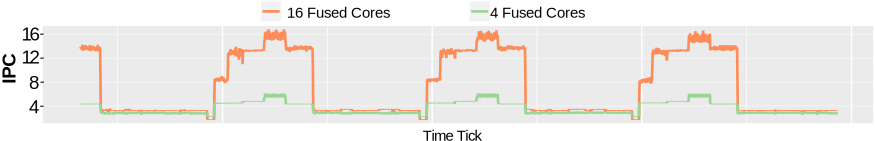
\includegraphics[width=\textwidth]{cases-paper/graphics/motivation/disp_opt_4_16_3.pdf}
    \caption{IPC of a typical benchmark (Disparity from SD-VBS) when executing on a fused 4 or 16 core processor.} 
    \label{fig:disp_ex}
	\vspace{1em}
\end{figure}
%\begin{figure}[t]
%    \centering
%    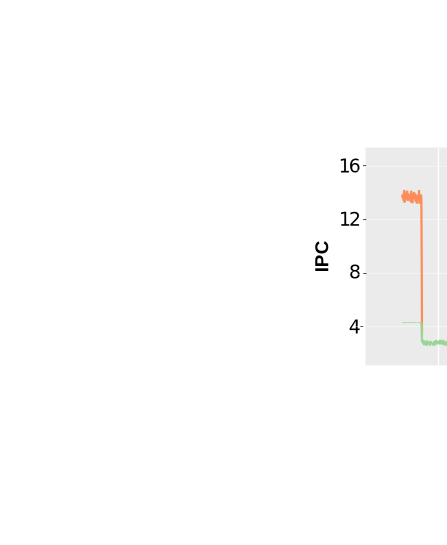
\includegraphics[width=\textwidth]{cases-paper/graphics/motivation/motiv3merge.pdf}
%    \caption{Example of ideal switching between 4 and 16 cores on a DMP for the Disparity benchmark.} 
%    \label{fig:ideal_switch}
%\vspace{2em}
%\end{figure}

Previous work in core fusion focuses on delivering performance improvements~\cite{ipek2007CoreFusion,kim2007tflex} and demonstrates how to predict static core fusion~\cite{micolet2016dmpstream}.
A static fusion fuses cores into a single logical core (LC) and executes a thread on this new core.
As evident from this prior work, fusion improves the performance of the program by maximizing speed.
However, as will be shown, static core compositions may not be the perfect match for all situations.

Figure~\ref{fig:disp_ex} plots the Instruction Per Cycle (IPC) performance variation over the execution of the \bm{Disparity} Benchmark from the San-Diego Vision Benchmark Suite (SD-VBS)~\cite{sdvbs} on core compositions of sizes 4 and 16 respectively.
IPC is a natural method of evaluating the performance of a core-composition as increasing the size of the composition should lead to a higher amount of instructions executing per cycle.
On 4 cores, the performance oscillates between an IPC of 2 and 6 depending on the phase while on 16 cores the IPC can be as high as 16.

In this Figure, the x-axis Tick represents a certain number of blocks that have been committed rather than being a measure of time in cycles.
This is why the high IPC phases for both core-compositions appear to last the same length of time even though the 16 core-composition executes the blocks faster.
In EDGE, a block is committed when it is no longer a speculative block and its memory and register operations have been committed back to memory or the register files.
The reason why number of blocks committed is used as a measurement of time is due to the fact that the number of blocks necessary to execute a program are independent of the size of a core-composition.

As can be seen in Figure~\ref{fig:disp_ex}, both the 4 and 16 core-compositions share the same IPC when it comes to the low IPC phase.
In a situation where the objective of the programmer is to maximise speed, without dynamic reconfiguration of the DMP, a static 16 core-composition will have to be used.
%Get actual energy estimations ot make this more clear
If the static 16 core composition is used, the DMP consumes 4 times as much energy to execute the low IPC phases compared to the 4 core-composition.
Thus, the static 16 core composition is considered energy inefficient during half the execution of the program.

On the other hand, if the DMP is reconfigured at runtime, the core-composition can switch to 4 cores when in the low-IPC phase to save on energy and switch to the 16 core composition when in the high IPC phase to maximise speedup.
In this situation, runtime reconfiguration allows to maximise speed whilst being energy efficient; a goal that cannot be achieved via static ahead of time configurations.

%Maybe, just maybe, add a graph showing how the size of the blocks change (need data on this).
\subsection{Code Optimizations}

When cores are fused they execute blocks of instructions in parallel on each physical core in the core composition, also known as a logical core (LC).
Having multiple cores in a composition can increase the amount of block level parallelism (BLP) that can be extracted out of a program.
A high amount of BLP leads to high IPC as each core in the LC executes their block in parallel.
As IPC is a more commonly used method of measuring performance, it is used throughout this chapter.
In order to obtain the best performance from an application, large blocks must be generated as this leads to a higher IPC on the LC as described in Chapter~\ref{chp:streamit}.
To summarise the reasons, which are also discussed in further details in Section~\ref{sec:lim_study}, larger blocks reduce the latency caused by having to fetch blocks for all the physical cores in the LC, thus improving performance.

Thus, optimisations that maximise block size will positively affect the performance of compositions.
This includes optimisations such as aggressive loop unrolling, inlining and replacing conditional statements with either software predication or architecture-level predication.
These optimizations are well known and do not require any structural modifications of the program.

\begin{figure}[t]
    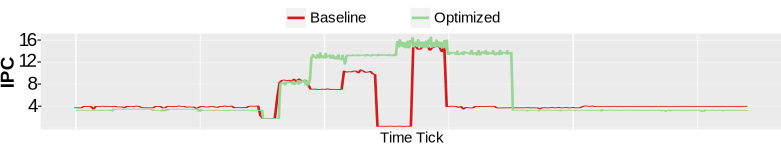
\includegraphics[width=\textwidth]{cases-paper/graphics/motivation/code_opt_3.pdf}
    \caption{Impact of loop transformations on fused cores for the Disparity benchmark.} 
    \label{fig:compmotiv}
\vspace{1em}
\end{figure}

Figure~\ref{fig:compmotiv} illustrates the impact of applying loop transformations on the \bm{Disparity} benchmark compared to a standard compiler not specifically tuned for the EDGE architecture.
The Figure shows the IPC performance of a 16 core composition with and without optimisations.
As can be seen, the impact of these transformations can be large, leading to an 12x improvement on IPC.
Figure~\ref{fig:compmotiv} shows that the optimisations allow the core-composition to sustain a high IPC phase longer than without the optimisations.
However, it also demonstrates that not all of the code in a program can be optimised, as the low-IPC phases do not change.
More details about the loop transformations are given in section~\ref{sec:opt} but this example illustrates the need for careful tuning of the compiler to achieve high performance on such an architecture.

%Find some citation for this
\subsection{Automating runtime reconfiguration}

Figure~\ref{fig:disp_ex} motivates the use of runtime reconfiguration to ensure that DMP can improve the performance of single threaded applications efficiently by minimising energy consumption.
Figure~\ref{fig:compmotiv} shows how modifying loops affects the performance in terms of IPC for a core-composition.
Using an API, a programmer could inform the hardware when to reconfigure by using specific functions or pragmas similar to OpenMP or OpenCL.
Whilst this may be considered a viable approach to applying runtime reconfiguration, automating the decision process is a better option.

Automating the process of reconfiguring the processor enables two advantages compared to manually determining when to reconfigure the processor.
The first advantage is that it removes the responsibility from the programmer: an automated runtime reconfiguration system can detect phases and adapt to them accordingly, using information gathered from previous traces.
Second, if ever the program is modified, this may require new profiling information to be generated to ensure that manual reconfiguration calls are correct.
If the reconfiguration is automated, then it can adapt automatically to any changes made to the source code.

\subsection{Summary}
This section has shown that programs exhibit phases with various amount of ILP available.
A dynamic multicore processor can take advantage of this property to fuse a large number of cores for the high-ILP phases and fuse a smaller number of cores when ILP drops to conserve energy.
The section also illustrated the importance of fine-tuned code transformations to achieve sustained performance and increase the potential for fusing cores.
The next section will study in more details the expected impact of fusion using an analytical model.



\section{A Study of Core Fusion}\label{sec:lim_study}
This section studies how block size and branch prediction limit the performance of core composition.
This enables a better understanding of what leads to good performance and how to determine regions of code that benefit from core composition.

\subsection{Branch Prediction}


As discussed in Chapter~\ref{chp:Background}, an EDGE based DMP accelerates a single thread by executing blocks of instructions from the same thread speculatively across several fused cores. 
In a core composition, the fetching scheme dictates that a core must fetch blocks until its instruction window is either full or cannot accomodate the newest block.
Once this requirement is met, the following block is sent to the next core in the composition.
If a core mispeculates a block, this can cause the entire composition to be flushed.
Thus core composition puts a strain on the branch predictor since efficiently using the cores depends on the prediction accuracy.

Depending on the sizes of the blocks and the number of cores in the composition, the branch predictor has to meet a different accuracy requirement to ensure all cores are being used efficiently.
In this case, efficiency is defined by cores in a composition successfully fetching correctly predicted blocks.
Given a core-composition of size \textit{CompSize}, the minimum branch prediction accuracy required to ensure efficient use of the composition can be determined using Formula~\ref{form:minpred} where \textit{BlocksInFlight} can be calculated using the equation~\ref{form:blocks}.

\begin{equation}\label{form:blocks}
BlocksInFlight(AverageBlockSize) = \begin{cases}
4, &\text{if } AverageBlockSize \le 32 \\
3, &\text{if } 32 < AverageBlockSize \le 64 \\
2, &\text{if } 64 < AverageBlockSize \le 96\\
1, &\text{if } 96 < AverageBlockSize\\
\end{cases}
\end{equation}

\begin{equation}\label{form:minpred}
PredAcc(ABS,CompSize)= \frac{BlocksInFlight(ABS) \times CompSize- 1}{BlocksInFlight(ABS) \times CompSize}
\vspace{1em}
\end{equation}

\textit{BlocksInFlight} represents the number of blocks that can execute on a single core in parallel.
There can be multiple blocks on a single core as the instruction window has four lanes per core.
In this thesis, the instruction window is 128 instructions wide, thus each lane can support a block of up to 32 instructions.
In Equation~\ref{form:minpred}, the -1 is due to the fact that when a program is executing the first block does not depend on a branch prediction, thus at any point during the execution of a program, there is a non-speculative block that does not need to predicted.

Figure~\ref{fig:req_pred} shows the expected prediction accuracy required to fully utilize a core composition given the average block size in flight.
In this figure, \textit{NumOfBlocksPerCore} is equal to four and \textit{MaxBlockSize} is 32.
Adding extra physical cores to a LC requires an increasingly accurate branch predictor, especially when the size of a block is under 50 instructions.
This provides two insights; first of all large LCs will need to run on code sections with less control flow as they are more sensitive to branch misspredictions.
Second of all, branch prediction can be a simple method of evaluating the current effectiveness of a LC.
Given a certain number of cores, if the prediction accuracy is under the limits presented in Figure~\ref{fig:req_pred} it can be easily determine that the LC is sub-optimal.

\begin{figure}[t]
    \centering
    \includegraphics[width=\textwidth]{cases-paper/graphics/limit_study/prediction_req.pdf}
    \caption{Required prediction accuracy for a logical core size to be efficient given an average block size.}
    \label{fig:req_pred}
	\vspace{1em}
\end{figure}

\subsection{Synchronization Cost}

For a program to execute correctly, the cores in a logical core (LC) must communicate when they have finished executing a block.
This ensures that the cores fetch blocks from the correct control paths and update memory and registers consistently.
A core may have to wait for other cores to commit before fetching a new block. 
The worst-case estimate of this stall is defined as the \textbf{Synchronization Cost}.

Blocks commit in a sequential fashion with the non-speculative block committing first and the most recent speculative block committing last.
If a core's instruction window is full then it must commit a block before it fetches a new one.
The Synchronization Cost, in cycles, is defined in equation~\ref{form:synccost} and is measured by averaging the overall number of cycles each fused core waits until it can continue to fetch and execute new blocks.
\textit{AvBlocksInFlight} represents the average number of blocks in flight on a single core in the LC.
This is a worst-case estimate as block sizes will fluctuate during the execution of a program.

\begin{equation}\label{form:synccost}
SyncCos(ABS,CompSize) = \frac{\sum_{CoreNumber=0}^{CompSize-1}\left(BlocksInFlight(ABS)\right) \times CoreNumber }{CompSize}
\end{equation}


Figure~\ref{fig:sync_cost} shows how many cycles the Synchronization Cost will be for a given LC and average block size.
The larger the block size the lower the Synchronization Cost is since cores fetch fewer blocks and wait less for other fused cores to finish committing.
Large LCs executing small blocks have a high Synchronization Cost. 
This indicates that large LCs should be avoided when dealing with smaller blocks as the Synchronization Cost outweighs the code execution.

\begin{figure}[t]
    \centering
    \includegraphics[width=\textwidth]{cases-paper/graphics/limit_study/sync_cost.pdf}

    \caption{Synchronization Cost in cycles for a given number of cores in a composition and an average block size.} %Each core has 4 lanes and each lane can fetch a block of up to 32 instructions. Lower is better.}
    \label{fig:sync_cost}
	\vspace{1em}
\end{figure}

\begin{figure}[t]
    \centering
    \includegraphics[width=0.8\textwidth]{cases-paper/graphics/limit_study/summary.pdf}
    \caption{IPC estimate given a logical processor size, average branch prediction and average block size for a dual-issue core. A higher IPC means better performance.}
    \label{fig:lm_summ}
\vspace{5mm}
\end{figure}


\begin{align}\label{form:wcetMath}
IPC(ASB,CS,BPredAcc) &= \bigg(\frac{ABS}{SyncCost(ASB,CS) + {\frac{ASB}{2}}}\bigg) \times BPredAcc \times CS
\end{align}


\paragraph{Summary}

This section estimates the worst-case IPC for a logical processor using Average Block Size, Average Branch Prediction, and Synchonization Cost.
Figure~\ref{fig:lm_summ} presented a worst-case estimate of IPC performance assuming each core can sustain an IPC of 2.
The figure is generated by assuming that cores can execute 2 instructions per block, and using the two previous formulas with different block sizes, accuracies and core composition sizes to generate estimated IPC values.
The formula used is defined in equation~\ref{form:wcetMath} where \textit{ASB} represents the average size of a block, \textit{CS} is the size of the composition and \textit{BPredAcc} is branch prediction accuracy that ranges from 0 to 1.
From what was previously explained, Figure~\ref{fig:lm_summ} shows us that to obtain optimal performance requires a high branch prediction accuracy and large blocks.
It shows that larger logical processors can easily under-perform; for example it can be seen that 16 fused cores often have IPCs under 15, meaning that each core has an IPC under~1.



\section{Experimental Setup}\label{sec:setup}
The previous section studied the performance potential for core fusion using an analytical model.
We now present the experimental setup used for the remaining parts of the paper where we conduct a thorough evaluation of core fusion with a cycle-level simulator.

\subsection{Benchmarks}

For this paper we study the performance of our Dynamic Multicore Processor (DMP) on a set of Vision Benchmarks designed for hardware and compiler research~\cite{sdvbs}.
The San Diego Vision Benchmark suite (SD-VBS) is composed of nine single-threaded C benchmarks ranging from image analysis to motion tracking.
These benchmarks represent state-of-the-art applications in image and vision recognition which are prevalent in embedded systems.

Vision applications typically have regular and simple control flow which enables the formation of large blocks of instructions.
Our processor relies on the ability to form large blocks to exploit ILP which makes these applications particularly well suited.
As the results will show, the phase length has minimal impact on energy savings when the reconfiguration overhead is low.

\subsection{Architecture and Simulator}

We use a cycle-level simulator of an EDGE-based Dynamic Multicore Processor~\cite{e2} whose core pipeline is verified against an RTL implementation within 5\%. 
This validation is done by running workloads on RTL and comparing the traces cycle-by-cycle with the software simulator.
The architecture and core fusion mechanics are similar to the work described in~\cite{kim2007tflex,putnam2010e2}.
We configure the simulator to model a 16 core multiprocessor, with 32 KB private L1 caches, and allow each core to fetch up to 4 blocks of instructions, 
and issue up to 2 instructions per block for a maximum of 64 blocks in flight.


\subsection{Fusing Cores} \label{sec:coresufion}

In this processor, the micro-architecture is distributed: register files, Load Store Queues (LSQs), L1 caches and ALUs all look like nodes on a network.
This means that when cores fuse together, this is similar to adding an extra node to the network.
When cores are fused, one of the cores will execute a non-speculative block from a single thread whilst all other cores execute speculative blocks that are predicted from the same thread.
For our study, we use a simple round robin policy to choose which core is going to execute the next speculative block.
When we start a new thread on a fused core the OS and runtime write the new core mapping to a system register.
The hardware then flushes these cores if they are not idle and sets the PC of the first block of that thread on one core in the logical processor and starts executing.

Fusing cores is therefore a lightweight process.
We estimate that switching the size of the logical-core (LC) results in a delay of 100 cycles on average.
The actual time varies based on the time it takes the cache coherence protocol to move the data around the memory system.
Section~\ref{sec:reconfoverhead} discusses in more details how latency affects energy efficiency and shows that dynamic core fusion is still highly beneficial even when considering overheads of 1,000 cycles.

\subsection{Compiler}
Each benchmark is compiled with the Microsoft C++ compiler for EDGE~\cite{e2}, with -O2 optimisations and using instruction predication for hyperblock formation~\cite{smith2006edge}.

\subsection{Measuring Performance and Power}

We run five simulations per benchmark, one for each LC size: 1, 2, 4, 8 and 16.
For each LC we record the IPC of the LC at an interval of 640 committed blocks.
We selected 640 committed blocks as it allows each core in a LC to execute enough blocks before taking the measurement.
This is due to the fact that the highest LC of 16 cores can execute up to 64 blocks at a time, thus recording performance after 640 blocks allows each core to have executed at least 10 blocks.
Using committed blocks as an interval allows us to easily compare each simulation as the total number of committed blocks does not change even if the LCs are different.

Due to the fact that we study an EDGE ISA~\cite{smith2006edge}, we cannot use McPAT to model power consumption as it differs from traditional CISC/RISC cores modeled in McPAT.
Instead we use a coarse grained power model where either a core is turned on or or it is off. 


\section{Code Optimizations}\label{sec:opt}
\lstset{
	backgroundcolor=\color{lbcolor},
	tabsize=2,
	rulecolor=,
	language=matlab,
        basicstyle=\tiny,
        upquote=true,
        aboveskip={1\baselineskip},
        columns=fixed,
        showstringspaces=false,
        extendedchars=true,
        breaklines=true,
        prebreak = \raisebox{0ex}[0ex][0ex]{\ensuremath{\hookleftarrow}},
        frame=single,
        showtabs=false,
        showspaces=false,
        showstringspaces=false,
        identifierstyle=\ttfamily,
        keywordstyle=\color[rgb]{0,0,1},
        commentstyle=\color[rgb]{0.133,0.545,0.133},
        stringstyle=\color[rgb]{0.627,0.126,0.941},
		numbers=left,
}

\begin{figure}[t]
\lstset{language=C,numbersep=4pt}
\begin{center}
\begin{lstlisting}
for(int i = 0; i < 1000; i++)
  for(int j = 0; j < 1000; j++)
     for(int k = 0;k < 5; k++)
         a[i][j] = a[i][j] * b[k][j];
\end{lstlisting}
\end{center}
\vspace{-2em}
\captionof{lstlisting}{Example of an inner-most loop which should be completely unrolled.}
\label{lst:small}
\vspace{-2em}
\end{figure}

This section describes optimisations focused on reducing control flow and expanding block sizes which is necessary for high performance as seen in section~\ref{sec:lim_study}.

\subsection{Loop Unrolling}
As seen in Chapter~\ref{chp:streamit} Section~\ref{sec:streamit:dse}, loop unrolling can be used to reduce the overhead of the loop header and to better expose Instruction Level Parallelism (ILP).
When dealing with tightly-knit loops, compositions may perform poorly due to the fact that they execute many small blocks, increasing the Synchronization Cost and the branch prediction accuracy requirements.
Unrolling loops reduces the number of blocks required to execute the loop and increases the size of the blocks, thus reducing the Synchronisation Cost and increasing ILP.
For example, the innermost loop in Listing~\ref{lst:small} should be completely unrolled and its outer loop unrolled to increase the block size.

There are certain factors limit the usefulness of loop unrolling.
In the evaluated EDGE architecture, blocks may not have more than 32 load or store instructions as described in Chapter~\ref{chp:Background} section~\ref{sec:edge_isa}.
Therefore unrolling memory intensive loops will not always drastically increase the size of a block if the block is composed mainly of load and store instructions, as the EDGE compiler will have to split blocks if they contain more than 32 load/store instructions.
However as it will generate blocks with fixed branches it reduces the strain on branch prediction.
Another issue is that unrolling loops with conditional statements may not help improve the size of the block as the conditional branches might still segment the new blocks.
So these loops should not be unrolled as they will lead to an increase in code size.


\subsection{Loop Interchange}
When dealing with nested loops there is one reason for interchanging the loops.
The case arises when interchanging the loop removes dependencies in the inner-most loop.
For instance, the dependency in listing~\ref{lst:dep} can be removed by interchanging the loops. 
This allows the compiler to unroll the inner loop efficiently, but also remove any kind of dependency between blocks.
Even if memory dependencies can be detected using a dependence predictor~\cite{chrysos1998storesets}, it can potentially serialise memory operations when multiple iterations of a loop are live.
Thus using loop interchange will reduce any potential data dependency and minimise core communication in a composition.


\begin{figure}[t]
\lstset{language=C,numbersep=4pt}
\begin{center}
\begin{lstlisting}
for(int i = 0; i < 1000; i++)
  for(int j = 0; j < 1000; j++)
      a[i][j] = a[i][j-1] * b[i][j];
\end{lstlisting}
\end{center}
\vspace{-1em}
\captionof{lstlisting}{Data dependency which can be removed via loop interchange.}
\label{lst:dep}
\vspace{1em}
\end{figure}

\subsection{Predication and Hyperblock Formation}
EDGE compilers must split blocks whenever control-flow is present~\cite{smith2006edge} as seen in Section~\ref{chp:bg:sec:edge} of Chapter~\ref{chp:Background}.
If a loop contains a conditional statement, the loop body has to be split in two unless if-conversion is applied.
Hyperblock formation aims to reduce branching and increase block size by combining two or more blocks into a single predicated block~\cite{smith2006edge}.
Hyperblocks reduce both synchronization cost and branch prediction requirements as discussed previously.
This is especially important in control-flow intensive loops where unrolling increases the number of conditional statements.
Hyperblock formation can be done automatically~\cite{smith2006edge} via a compiler flag provided by the EDGE compiler.
However, as of the writing of this thesis, a block can only support a single predication, thus hyperblock formation cannot be paired with loop unrolling for example.

\begin{figure}[t]
     \centering
     \includegraphics[width=\textwidth]{cases-paper/graphics/Exploration/ipc_comp.pdf}
\vspace*{-8mm}
     \caption{Average IPC using the optimal sized logical-core, with and without optimisations. Higher is better.}
     \label{fig:ipccom}
     \vspace{0.5em}
\vspace{5mm}
    \centering
    \includegraphics[width=\textwidth]{cases-paper/graphics/Exploration/comp_speed.pdf}
\vspace*{-8mm}
    \caption{Speedup from using code-optimisations over baseline source code using the same optimal sized logical-core.}
    \label{fig:speedcomp}
\vspace{5mm}
\end{figure}

\subsection{Optimisation Methodology}
While the optimisations described above and their tuning would be easy to implement in a compiler, this thesis did not have access to the compiler's source code.
Therefore the source code of the benchmarks is modified by manually interchanging or unrolling loops.
In the case of predication and hyperblock formation, simple if-then-else statements are converted into ternary operators whenever possible.
Statements are also re-ordered within the body of a loop to avoid having control flow in the middle of the body.
For loop unrolling, the loops were unrolled to fit a single block.
The source code modifications are then verified to have the intended effect by disassembling the binary file produced by the compiler.
On average there are between 0 and 12 loops modifications depending on the benchmark.

\subsection{Results}
First the best static core composition using the optimised code is compared with the unmodified code, both version compiled with \texttt{-O2} which is the highest optimisation setting for the EDGE compiler.
Figure~\ref{fig:ipccom} shows the resulting IPC for the baseline case and the optimised benchmarks when run on a core with the optimal number of composed core to maximise performance.
The IPC of the baseline is very low for the majority of the benchmarks which might give the impression that core composition is rather inefficient.
However, after applying the simple optimisations described above, the average IPC is significantly increased in many cases.

Since optimisations change the total number of instructions, the actual speedup obtained using cycle count is also shown in Figure~\ref{fig:speedcomp}.
As can be seen, benchmarks \bm{MSER} and \bm{Multi-NCut} do not perform any differently.
This is due to the fact that none of these optimisations can be successfully applied on these benchmarks, as the loops cannot be interchanged or unrolled effectively, these applications are discussed in greater detail in Section~\ref{sec:expl}.
For the other benchmarks there is a significant improvements of up to 12$\times$ for \bm{Sift} when the optimisations are applied.
It is important to note that, whilst often the increase in IPC correlates with the speedup, this is not always the case.
In these situations, this is due to the fact that some of the optimisations also reduced the amount of computation required to complete the program; this is the case for \bm{Localization}, \bm{Sift} and \bm{TextureSynthesis}.
These benchmarks benefit from other source code modifications such as forced inlining for \bm{Localization} and \bm{TextureSynthesis} and loop invariant code motion for \bm{Sift} which were also applied manually.

\paragraph*{Summary}

Overall, this section shows that classical loop transformations can have a large impact on the performance of composed cores.
Without these optimisations, it would be more difficult to motivate the use of core fusion even at a static-level as the IPC does not deviate enough from a single core.


\begin{figure*}[t]
    \centering
    \includegraphics[width=1\textwidth]{cases-paper/graphics/Exploration/ipcs_16_2.pdf}
    \vspace*{-8mm}
    \caption{IPC as a function of time for each benchmark when run on 16 fused cores.}
    \label{fig:sxt}
\vspace{5mm}
\end{figure*}

\vspace{5mm}
\section{Benchmark Exploration}\label{sec:expl}
This section explores how core fusion affects the performance of the SD-VBS benchmarks.
First a phase analysis is performed, followed by a study of the IPC variation for static core fusion.
Then the use of dynamic core fusion is motived by using the information gathered.


\begin{figure}[t]
    \centering
    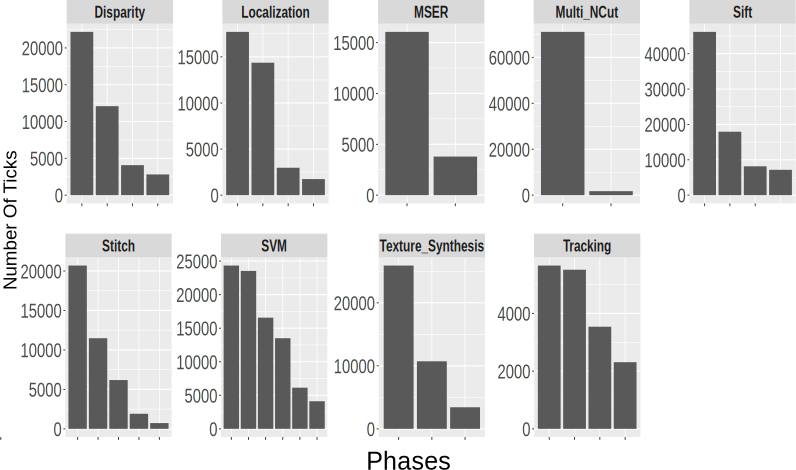
\includegraphics[width=1\textwidth]{cases-paper/graphics/Exploration/clusters3.pdf}
    \caption{Number of phases determined for each benchmark using kMeans clustering and their distribution.}
    \label{fig:clust}
		\vspace{5mm}
\end{figure}


\subsection{Phase Detection}
Figure~\ref{fig:sxt} presents the IPC performance through time for all the benchmarks when using a logical core (LC) composed of 16 cores.
The IPC is calculated for each time tick, which is set at interval of 640 blocks committed.
The IPC varies a lot for some of the benchmarks such as \bm{Disparity} or \bm{Localization} where dynamic fusion is expected to be especially good.
For other, such as \bm{Multi\_NCut}, the execution is dominated by a single long phase with constant IPC, which will clearly show no benefit from using dynamic fusion.

To better understand how dynamic core fusion improves performance, either by improving speedup or reducing energy, this section begins with a study of how each benchmark features different phases during their execution.
For every benchmark the IPC results of 16,8,4,2,1 fused cores are regrouped and kMeans clustering is applied to determine phases.
This process is only done for the purpose of exploring this set of benchmarks.
Intervals that exhibit similar IPC values when run on different core counts are classified in the same cluster.
In order to find the correct number of clusters the Sum of Square Errors (SSE) is plotted for a given cluster size from 1 to 15 and determine the optimal cluster to be in the elbow in the plot~\cite{everitCluster2001}.

Figure~\ref{fig:clust} shows us the optimal number of clusters for each benchmark and the frequency of each cluster.
The data can be corroborated with the information found in Figure~\ref{fig:sxt}.
For example, benchmarks \bm{MSER} and \bm{Multi\_NCut} feature two phases, with one dominating phase.
This means that it will be impossible to obtain any kind of performance improvements through dynamic reconfiguration.
For all the other benchmarks, they each have at least two dominant phases.
Since each phase is a cluster of similar IPC values, having two or more clusters will result in a higher chance of benefiting from dynamic core fusion.


\begin{figure}
    \centering
    \includegraphics[width=1\textwidth]{cases-paper/graphics/Exploration/stddev2.pdf}
    \caption{Comparing average, smallest and greatest IPC for each SD-VBS benchmark using logical-core size of 16.}
    \label{fig:stddev}
		\vspace{5mm}
\end{figure}

\begin{figure}[t]
    \centering
    \includegraphics[width=1\textwidth]{cases-paper/graphics/Exploration/SizeBuckets.pdf}
    \caption{Distribution of block sizes for each benchmark. The sizes were clustered in buckets equivalent to number of lanes occupied.}
    \label{fig:block_sizes}
	\vspace{5mm}
\end{figure}
\subsection{Static Core Fusion Exploration}

Figure~\ref{fig:stddev} shows how the average Instructions Per Cycle (IPC) changes as the size of a LC is increased, going in powers of 2 from 1 to 16 fused cores.
It can be seen that, for most benchmarks, fusing more cores provides an increase in IPC performance.
Benchmarks \bm{Disparity}, \bm{Localization}, \bm{Sift}, \bm{Stitch}, \bm{Texture Synthesis} and \bm{Tracking} all at least observe a speedup of 2x when using core fusion.

However increasing the size of a LC is not always beneficial as can be seen in benchmarks \bm{Localization}, \bm{MSER}, \bm{Multi\_NCut}, \bm{Stich}, and \bm{SVM}.
For benchmarks \bm{Localization} and \bm{Stitch} the performance increases when fusing up to 8 cores, where-as \bm{MSER} and \bm{Multi\_NCut} never benefit from core fusion. 
Referring back to Figures~\ref{fig:sxt} and~\ref{fig:clust}, \bm{MSER} and \bm{Multi\_NCut} feature one dominating long phase, both performing poorly.
Figure~\ref{fig:block_sizes} shows the distribution of block-sizes for each of the benchmarks.
As fine-grained sizes do not matter as much as overall number of lanes being occupied, the block sizes were clustered into groups which represent how ever many number of lanes will be occupied (one lane may execute a block of up to 32 instructions).

Figure~\ref{fig:block_sizes} helps explain why benchmarks \bm{MSER} and \bm{Multi\_NCut} do not perform any better with core-fusion.
For both cases, not only do they have a single detected phase, but both are predominantly formed of blocks that will occupy a single lane.
In fact, the most frequent block in \bm{MSER}, comprising 21\% the total executed blocks are comprised of only 8 instructions, whilst 31\% of \bm{Multi\_NCut}'s blocks are of 28 instructions.
Having such small blocks will always increase both the \textit{SynchronizationCost} and the branch-prediction requirements.
For \bm{MSER}, the fact that an important percentage of blocks are only 8 instructions long signifies that the overhead of fetching enough blocks for a large core-composition and the synchronization cost for committing them outweighs executing the blocks on a single core.
The reason there is no degredation of performance is due to the fact that when fusing a high amount of cores, if the overhead of fetching the blocks outweighs the time required to execute them, cores will simply not execute blocks.
For example, fusing 16 cores and executing \bm{MSER} may in fact result in a single core being used due to it executing blocks faster than it being able to dispatch the blocks to a next core.
Hence, in this case, \bm{MSER} would be wasting a lot of energy trying to use 16 cores in a composition, whilst effectively only executing on a single core. 
This explains the lack of scaling for these two benchmarks.

Figure~\ref{fig:stddev} also shows the standard deviation of the IPC for each given LC size represented by the grayed out areas.
For example, running the \bm{Disparity} benchmark on a LC of 16 cores, it can be observed that an average IPC of 8.3 with a standard deviation of 5.2.
The standard deviation for 16 cores shows that the performance can drop down to 2.5.
An IPC of 2.5 when using 16 cores is very inefficient as this represents 0.1 of an instruction per cycle for each core.
Using a LC of size 4 for the \bm{Disparity} benchmark we achieve an average of 4.1 with a standard deviation of 1.2.
Thus, if the logical-core could change size, there is a possibility that this could reduce the overall energy consumption of the system by switching from 16 to 4.

Overall, most benchmarks that benefit from large logical-cores will also be met with important standard deviations of IPC performance.
The high standard deviation is evidence of performance phases found in each application which are likely to benefit from dynamic adaptation.

\begin{figure}
     \centering
     \subfloat[][Disparity]{\includegraphics[width=0.5\textwidth]{cases-paper/graphics/Pareto/DispN3.pdf}\vspace*{-4mm}\label{subfig:disp}}
     \subfloat[][Localization]{\includegraphics[width=0.5\textwidth]{cases-paper/graphics/Pareto/LocN3.pdf}\vspace*{-4mm}\label{subfig:loc}}\
     \subfloat[][MSER]{\includegraphics[width=0.5\textwidth]{cases-paper/graphics/Pareto/MSERN3.pdf}\label{subfig:mser}}
     \subfloat[][Multi\_Ncut]{\includegraphics[width=0.5\textwidth]{cases-paper/graphics/Pareto/MultiN3.pdf}\label{subfig:mult}}\
     \subfloat[][Sift]{\includegraphics[width=0.5\textwidth]{cases-paper/graphics/Pareto/SiftN3.pdf}\label{subfig:sift}}
     \subfloat[][Stitch]{\includegraphics[width=0.5\textwidth]{cases-paper/graphics/Pareto/StitchN3.pdf}\label{subfig:stitch}}\
     \subfloat[][SVM]{\includegraphics[width=0.5\textwidth]{cases-paper/graphics/Pareto/SVMN3.pdf}\label{subfig:svm}}
     \subfloat[][Texture\_Synthesis]{\includegraphics[width=0.5\textwidth]{cases-paper/graphics/Pareto/TextN3.pdf}\label{subfig:text}}\\
     \subfloat[][Tracking]{\includegraphics[width=0.5\textwidth]{cases-paper/graphics/Pareto/TrackingN3.pdf}\label{subfig:track}}
     \caption{Time (x-axis) vs. Energy (y-axis) tradeoffs using Static and Dynamic Composition Schemes.}
     \label{fig:paretos}
\end{figure}
\newpage

\section{Dynamic Core Fusion}\label{sec:dynamic}
This section discusses a dynamic core composition scheme that is created by generating traces of the ahead-of-time static compositions.
The section first describe how the traces are generated for the dynamic core composition schemes.
Before the analysis two types of static core composition are defined:

\begin{itemize}
	\item \textbf{Static Benchmark} (SB): A fixed fused-core which is optimal for a unique benchmark.
\vspace{-1.2em}
	\item \textbf{Static Suite} (SS): A fixed fused-core which represents the average best for the entire suite of benchmarks. This represents the baseline for the chapter.
\end{itemize}

The reason \textbf{Static Suite} is used as a baseline is due to the fact that it represents a configuration choice at design time.
It is the equivalent of hardware designers analysing the requirements of a processor based on the type of applications it will be executing.
This is better than using a single core as a baseline, as a single core will always represent the slowest execution time whilst also consuming the least amount of energy.
\textbf{Static Benchmark} on the other hand represents the ability to compose cores statically ahead of time; which is an extra step of flexibility compared to \textbf{Static Suite}.

The static core-composition scheme \textit{SS} is compared to the results obtained for the dynamic one for the SD-VBS benchmarks.
This is followed by a closer analysis of the dynamic core composition objective: optimising speed whilst reducing energy consumption.

\begin{figure}[t]
    \centering
	\includegraphics[width=1\textwidth]{cases-paper/graphics/exploration/trace-gathering.pdf}
    \caption{Overview of how traces are gathered to generate dynamic core composition traces.}
    \label{fig:tracegraph}
	\vspace{1em}
\end{figure}

\subsection{Creating Dynamic Core Composition Traces}

Dynamic core composition enables the ability to change the number of cores for each time tick (an interval of 640 committed blocks) during the execution of a program.
In order to explore the different performance and energy trade-offs that are possible to achieve with this technique, traces of execution for the application are collected.
Figure~\ref{fig:tracegraph} is a visual overview of how dynamic traces are collected.
First the application is executed on 1,2,4,8 and 16 composed cores and the performance is recorded for each time tick of 640 committed blocks.
Using these 5 traces, dynamic executions using any of the 5 different compositions can be constructed to generate dynamic traces.
For this chapter, the dynamic trace are generated based on maximising speed whilst minimising energy consumption.

To simplify the exploration process, time ticks that are attributed to the same phase are always given the same number of cores.
This is done to reduce the search space as on average there are 48,494 ticks which results in an average of $5^{48,494}$ different possible executions.
Since the maximum number of clusters found is 7 (for SVM), a maximum of $5^{7} = 78,125$ different dynamic execution traces can be built.
This is why creating dynamic core-composition out of traces is preferred to running all potential dynamic configurations via the simulator.
All applications run for a couple hundred million cycles, which often takes a couple of hours to execute.
As the amount of dynamic reconfigurations is high for some benchmarks, using traces to simulate dynamic reconfiguration is a very large time-save.

When the size of the core composition is switched, the performance of that composition from its respective trace file is used and an extra 100 cycle penalty is added for switching the size.
This 100 cycles is the overhead of reconfiguring the processor at runtime, the effect of the reconfiguration latency is discussed in further detail later on in this section.
The reconfiguration is a lightweight process as described in Chapter~\ref{chp:Background} section~\ref{sec:edge_arch} that involves informing the cores that they belong to a composition, which requires a write to a system register and potentially flushing pipelines if the cores are executing other threads.
As in this chapter, cores will never be executing other threads, flushing is not necessary, thus the l00 cycles to inform cores is an appropriate penalty and has been used in previous studies on DMPs~\cite{pricopi2012bahurupi}.
With all these different dynamic core composition traces, the optimal schemes for efficiently maximising speed can be found.

\begin{figure}[t]
    \centering
	\includegraphics[width=1\textwidth]{cases-paper/graphics/pareto/pareto_best.pdf}
\vspace{-1em}
    \caption{Time (x-axis) vs. Energy (y-axis) trade-offs using Static and Dynamic Composition Schemes.}
    \label{fig:paretos}
	\vspace{1em}
\end{figure}

%\begin{figure}[t]
%     \centering	%
%	 \vspace{-1em}
%     \subfloat[][Disparity]{\includegraphics[width=0.33\textwidth]{cases-paper/graphics/Pareto/DispN3.pdf}\vspace*{-4mm}\label{subfig:disp}}
%     \subfloat[][Localization]{\includegraphics[width=0.33\textwidth]{cases-paper/graphics/Pareto/LocN3.pdf}\vspace*{-4mm}\label{subfig:loc}}
%     \subfloat[][MSER]{\includegraphics[width=0.33\textwidth]{cases-paper/graphics/Pareto/MSERN3.pdf}\label{subfig:mser}}\
%	 	 	 \vspace{-0.5em}
%
%     \subfloat[][Multi\_Ncut]{\includegraphics[width=0.33\textwidth]{cases-paper/graphics/Pareto/MultiN3.pdf}\label{subfig:mult}}
%     \subfloat[][Sift]{\includegraphics[width=0.33\textwidth]{cases-paper/graphics/Pareto/SiftN3.pdf}\label{subfig:sift}}
%     \subfloat[][Stitch]{\includegraphics[width=0.33\textwidth]{cases-paper/graphics/Pareto/StitchN3.pdf}\label{subfig:stitch}}\
%	 	 	 \vspace{-0.5em}
%
%     \subfloat[][SVM]{\includegraphics[width=0.33\textwidth]{cases-paper/graphics/Pareto/SVMN3.pdf}\label{subfig:svm}}
%     \subfloat[][Texture\_Synthesis]{\includegraphics[width=0.33\textwidth]{cases-paper/graphics/Pareto/TextN3.pdf}\label{subfig:text}}
%     \subfloat[][Tracking]{\includegraphics[width=0.33\textwidth]{cases-paper/graphics/Pareto/TrackingN3.pdf}\label{subfig:track}}
%     \caption{Time (x-axis) vs. Energy (y-axis) tradeoffs using Static and Dynamic Composition Schemes.}
%     \label{fig:paretos}
%	 	 	 	 \vspace{1em}
%\end{figure}

\subsection{Dynamic Core Composition}
Figure~\ref{fig:paretos} shows the trade off between time (cycles) and energy using either a static ahead of time or dynamic (re)-configuration.
The dotted line represents the static core composition scheme for the benchmark whilst the solid line represents the Pareto Front of all the dynamic core composition traces.
The vertical line represents the amount of energy that can be saved from using a dynamic core composition scheme that matches the same speed as the best static scheme.
The Pareto Front is constructed by assigning different core composition sizes to a phase and recording the execution time in cycles and energy consumption.
For a given cycle count, the reconfiguration scheme that leads to the smallest energy consumption is chosen to be a point in the Pareto Front.

Figure~\ref{fig:paretos} demonstrates how static core-composition fails to maintain good energy efficiency as speed is improved.
For example, \bm{Disparity} is fastest on 16 fused cores, but has an 1.63x increase in energy consumption for a 1.22x improvement in speed.
This is due to the fact that larger core compositions do not result in linear speedups, and thus consume more energy than a smaller core composition.
When using the dynamic scheme, it is clear that energy consumption increases at a slower rate when increasing speed.
In this case the number of cores is adapted to the current phase, using just enough cores to maintain high performance without wasting energy.

Figure~\ref{fig:paretos} also shows how very few applications get faster execution times with dynamic core composition.
The main program that does perform better execution wise with dynamic core composition is \bm{Localization}.
In the case of \bm{Localization}, the fastest execution time using static core-composition comes from a logical core of size 8.
However, there are certain phases that perform better with 16 cores, and thus, dynamic core composition in this situation can lead to faster execution times.
Overall, for these benchmarks, most have their fastest execution times with a static core-composition.
Dynamic reconfiguration is therefore mainly used to limit the energy consumption.

\subsection{Optimising for Speed} \label{sec:dyn:speed}

In this section the dynamic scheme is defined to be one that matches the same speed performance as the fastest static core composition for the benchmark: \textbf{DSpeed}.
This is equivalent to the vertical line found in Figure~\ref{fig:paretos}.
This scheme is used to demonstrate how dynamic reconfiguration can achieve the same speed as the static configuration whilst reducing energy consumption.

Figure~\ref{fig:speedres} shows the speedup of \textbf{DSpeed} and Static Best (SB) and the respective energy consumption.
The results are normalised against the performance of Static Suite (SS), which is 8 cores fused.
The SS core count is obtained by averaging the number of cores that leads to the fastest execution time for each benchmark.
The execution times for \textbf{DSpeed} and SB are the same as the dynamic scheme designed to match the static best's execution time.
As can be seen some benchmark perform better when using benchmark specific core compositions rather than SS.
Both \bm{Disparity} and \bm{Sift} obtain a 1.25x speedup when using the SB scheme whilst \bm{Tracking} benefits from a 1.10x speedup.
This reconfirms the concept that even static core-composition is a feature that leads to performance improvements over design time configurations.

\begin{figure}[t]
    \centering
	\includegraphics[width=1\textwidth]{cases-paper/graphics/results/speed_bars3.pdf}
\vspace{-1em}
    \caption{Maximising speed for all the SD-VBS benchmarks. For Speedup, higher means better, for Energy, lower is better.}
    \label{fig:speedres}
	\vspace{1em}
\end{figure}

When looking at the Energy graph of Figure~\ref{fig:speedres}, it is clear where the SS scheme fails.
Benchmarks \bm{MSER} and \bm{Multi\_NCut} feature very little improvement when using core composition, if any, therefore SS will perform very poorly when it comes to energy consumption for the benchmarks.
In the case of those benchmarks, the energy consumption is over 2x less on SB than it is on SS.
In this situation, SS is analogous to designing a large physical core meant to extract a lot of IPC for single-threaded performance and executing low IPC benchmarks on it.
This core will end up consuming too much energy and lead to low performance increases.
SB already shows the advantages of designing smaller, simpler physical cores which can be composed ahead of time.
For applications such as \bm{MSER} or \bm{Multi\_NCut}, a single low energy core suffices whereas \bm{Disparity} and \bm{Tracking} benefit from large compositions for better speedup.

However, SB is still not an optimal solution. 
For the benchmarks \bm{Disparity}, \bm{Sift}, \bm{Texture\_Synthesis} the energy consumption is much higher.
This is due to the fact that these benchmarks perform best on a 16-core system, however as seen in Figure~\ref{fig:stddev}, the variation in performance always increases when fusing this many cores.
In this situation, whilst 16 cores does result in the fastest execution times, the energy consumption is higher than SS.
This shows the limitations of static configuration overall, whether it be at design time or ahead of time: the lack of flexibility means that compromises have to be made.
In the case of aiming for the fastest execution times energy consumption may increase.

%More here
The dynamic reconfiguration \textbf{DSpeed} scheme always performs better than the SB scheme in terms of energy consumption and can even match the SS scheme on energy consumption whilst improving speed such as in the \bm{Sift} benchmark.
For the \bm{Localization} benchmark, the \textbf{DSpeed} matches the performance of both the SB and SS whilst reducing energy consumption by 65\%.
By using \textbf{DSpeed}, the energy consumption can be reduced by 42\% compared to both SB and SS without impacting performance.
This illustrates the greatest advantage of using a DMP since the number of composed core can be adapted continuously depending on the amount of ILP available.

\subsection{Reconfiguration Latency} \label{sec:reconfoverhead}

\begin{figure}[t]
	\begin{minipage}{.5\textwidth}
	\includegraphics[width=.9\linewidth]{cases-paper/graphics/Exploration/condensed_clust.pdf}
    \caption{Average number of cycles without switching.}
    \label{fig:avlen}
	\end{minipage}%
	\begin{minipage}{.5\textwidth}
	\hfill
	\includegraphics[width=.9\linewidth]{cases-paper/graphics/Exploration/latency_2.pdf}
    \caption{Energy savings and number of switches as a function of the switching latency in cycles.}
    \label{fig:enlatency}
\end{minipage}
\vspace{5mm}
\end{figure}

%Check if th
Up until now, the chapter has assumed a reconfiguration latency of 100 cycles whenever dynamic reconfiguration occurs as explained in Chapter~\ref{chp:setup}.
This section studies the impact of a larger reconfiguration overhead on energy savings.
First, figure~\ref{fig:avlen} shows the average phase length for each benchmark when maximising energy savings while maintaining performance (\textbf{DSpeed}).
As can be seen, the majority of the benchmarks run for long period of several tens of thousands of cycles before any switching occurs on average.
Therefore, even if the reconfiguration latency is increased to a larger value (\eg 1,000 cycles), its impact might be minimal.
For these applications, the phase length is also tied to the size of the input, the phases may increase when working on inputs such as high definition images.

Furthermore, there is always the option to reconfigure less often, in the case where a change in configuration only brings marginal reduction in energy.
In such case it might be more beneficial to keep running on the slightly less optimal configuration than paying a cost for reconfiguration.
Figure~\ref{fig:enlatency} illustrates this perfectly, showing how energy behaves as a function of the reconfiguration overhead (averaged across benchmarks).
For each latency value, the best trace of reconfiguration is determined to keep performance equal to the best static configuration while minimising energy (\textbf{DSpeed}).
The left y-axis expresses the energy savings relative to the static scheme, while the right y-axis shows the total number of switches.
The energy savings remains high up to a latency of 1,000 cycles, with a noticeable decrease in the number of switches.
For latency values over 1,000 cycles, the energy savings drop considerably, with very little switching occurring.
This data shows that even if the reconfiguration overhead is 1,000 cycles, average energy savings of 38\% are possible compared to 42\% when the overhead is 100 cycles.

\paragraph*{Summary}

Overall, dynamic core composition will always lead to higher speedup with lower energy consumption compared to a fixed configuration.
This is due to the presence of phases in applications that the dynamic scheme can exploit to reduce wasting energy in low ILP phases.
This section has shown that maximising speed can be highly energy inefficient when using a static composition and that a dynamic scheme can help reduce energy consumption by 42\% on average.




\section{Linear Regression Model}\label{sec:model}
The previous section showed that dynamically reconfiguring the processor can help reduce energy consumption whilst still achieving the same execution time as the fastest ahead of time configuration.
In order to benefit fully from dynamic core-composition two solutions are possible; either the programmer must go through the code and manually determine when to change the composition or an automatic scheme can be deployed.
This section now presents a learning scheme that is used to exploit the large energy savings available.
The main idea is to monitor at runtime some performance counters and make a decision at a regular interval on how to reconfigure the cores.
For this purpose, a model is trained offline using the data collected and presented earlier in the chapter.
Once trained, the model predicts the optimal number of cores based on the performance counters from the previous time interval and reconfiguration occurs if it is different from the current number of cores.

\begin{figure}[t]
    \centering
	\includegraphics[width=1\textwidth]{cases-paper/graphics/other/model3.pdf}
	\vspace{-2em}
    \caption{Linear Model.}
    \label{fig:linmod}
\end{figure}
\subsection{Model}

As the decisions are made at runtime, a lightweight model that is able to predict the correct configuration that can be integrated in hardware is necessary.
Linear regression, which makes predictions using a weighted sum of the input feature, has been demonstrated to be useful for predicting processor performance~\cite{Joseph2006LinReg}.
It is chosen as it has been as it can easily be implemented in hardware~\cite{lee2006linreg,Lukefahr2012Composite} and has a low overhead when computing the sum.
The model is trained offline using the traces gathered from the prior analysis for the \textbf{DSpeed} scenario which maximises energy savings while maintaining performance.

Figure~\ref{fig:linmod} is a shows how the linear model is trained.
The dataset consists of a set of four input features (average block size, and percentage of integer, floating point and load operations) and the optimal number of cores for each time tick for each program.
These features are chosen as they are easy to extract from the hardware.
The reason stores are not in the feature vector is due to the fact that a block is comprised only of integer, floating point, load and store operations.
Therefore, when building the model, a correlation analysis determined that stores correlate with other features and selects to remove it as a variable.
 % a single data point is created per phase, averaging the features of all the ticks in a phase, resulting in a total of 34 pairs of optimal core number and features.

To speedup the learning process, for each benchmark the features of all the ticks in a phase were averaged out to create a single data point, which is comprised of an IPC value, and the features described in Figure~\ref{fig:linmod}.
This averaging out leads to 34 data points for all the benchmarks.
The training consists of finding the weights that minimise the error when predicting the optimal number of cores to use across all time ticks and benchmarks.
Since only core configurations which use a power of two number of cores are considered, the linear model is built to predict the logarithm (base 2) of the number of cores.
The prediction is rounded up to the nearest integer in the interval $[0,4]$.
The following equation represents the trained linear model which can be used to make prediction:
\vspace{-1em}
\begin{align*}
  log_2(\textbf{\#cores}) = & -7.7\ +\ 0.028 \cdot \textbf{avgBlkSze}\ +\ 0.075 \cdot \textbf{\%int\_ops}\ +\\
 &0.069 \cdot \textbf{\%fp\_ops}\ +\ 0.21 \cdot \textbf{\%ld\_ops}
\end{align*}

It is important to note that this model was not used during the validation, as cross-validation (see Chapter~\ref{chp:Background}) was used to evaluate it.
Instead, this represents a model where the data from all programs is used.
For instance, if at runtime an average block size of 6 instructions, and 77\%, 1\% and 18\% of integer, floating point and load operations, respectively, then the predicted value will be 2.092.
Rounded up to the nearest integer value, 2, the optimal number of cores predicted will, therefore, be 4.

As can be seen, the largest weight is on the percentage of loads operations.
This is due to different reasons, mainly execution time and the fact that Load-Store Queues are fused.
When it comes to execution time, loads may take from 3 to 128 cycles depending on whether or not it is a cache miss or hit.
Whether it is a cache hit or miss, a block that takes longer to execute will often minimise the \textit{SynchronisationCost} penalty.
A block composed mainly of integer or floating point operations will often result in shorter execution rates; thus may execute faster, making it harder for large logical cores to improve performance.

More discussion on how the time it takes to execute a block influences the performance of core compositions is discussed in Chapter~\ref{chp3}.
The other reason loads have the largest weight is due to the fact that loads can be fired independently to the Load-Store Queue.
Unlike stores that depend on previous memory instructions blocks being committed, loads can be fired with less overhead.
As data can be speculatively fetched, load instructions can receive data from other cores before the data is stored, speeding up executions.
By increasing the core count on load heavy blocks this will improve performance more reliably due to cores being able to issue loads in parallel.

\begin{figure}[t]
    \centering
	\includegraphics[width=1\textwidth]{cases-paper/graphics/results/lr_speed3.pdf}
    \caption{Performance results for maximising speed for the SD-VBS benchmarks using the linear regressor (LR) model. The results are normalised against the Static Suite core composition.}% For Speedup, higher means better, for energy lower is better.}
    \label{fig:speedlr}
	\vspace{1em}
\end{figure}

%explain why MSER here is bad. Most likely because it over-estimates because some features in the vector don't describe the performance in the application.
%This is most likely due to the branch prediction/.
\subsection{Results}

To evaluate the performance of the model leave-one-out cross-validation  is used; it is a standard machine-learning methodology which tests the model using not seen during training.
For instance, if the model is tested for one program, let say \textit{Disparity}, the model is then trained using the dataset from all the other programs combined.
Then the resulting trained linear model is used to predict the optimal core number for each time tick of the disparity program and report the performance achieved.

Figure~\ref{fig:speedlr} shows the performance in terms of speed and energy that is achieved using the linear model normalised by a fixed static configuration.
The fixed configuration maximised performance across all the benchmarks using 8 cores and is the same as in the previous results presented in figure~\ref{fig:speedres}.
On average, the linear regressor model is able to consume 37\% less energy compared to the 8 cores fixed configuration and is able to exactly match its speed.
The main outlier is \bm{MSER} where the linear regressor consumes over 2x more energy than \textbf{DSpeed}.
This is due to the fact that \bm{MSER} is a benchmark where the branch prediction is poor as previously mentioned in Table~\ref{tab:sd-vbsbpred}.
Indeed, \bm{MSER} has an average branch prediction of 85\% compared to the average of 95\%.S
As \bm{MSER} tends to have very small blocks, the branch prediction makes it very difficult to ever efficiently use even a core composition of size 2.
This benchmark is therefore an outlier compared to the rest of the set, as it is the branch prediction causing incorrect predictions from the linear regression.

The performance is also compared with the best possible choice of dynamic reconfiguration, \textbf{DSpeed} which acts as an Oracle.
As can be seen, the linear model is able to exploit similar energy savings to the \textbf{Dspeed} scheme in most cases.
On average it reduces energy by 37\%, which is within 5\% of the 42\% achievable by the \textbf{Dspeed} scheme.
These results show that it is possible to implement a simple realistic lightweight scheme which offers large energy savings.


\section{Related Work}\label{sec:related}

\paragraph{Reconfigurable Processors}

ElasticCore~\cite{tavanaElastic} proposes a morphable core that uses dynamic voltage and frequency scaling (DVFS) and microarchitectural modifications such as instruction bandwidth and capacity.
They propose a linear regressor model to determine reconfiguration, which uses more runtime information than ours, such as branch prediction and cache misses.
Overall Tavana et al's architecture is 30\% more energy efficient than a big.LITTLE architecture.

In~\cite{dubach13dynamic} they also propose a similar core architecture that modifies microarchitectural features.
They provide extensive analysis of SPEC 2000 benchmarks and demonstrate that machine learning and dynamic adaptation can double the energy/performance efficiency compared to a static configuration.

MorphCore~\cite{khubaibMorphCore2012} focuses on reconfiguring a core for thread level parallelism.
It switches between out-of-order (OoO) when running single threaded applications and an in-order core optimised for simultaneous multi threading (SMT) workloads.
This provides an opposite solution to our DMP: providing a large core made for ILP that can be modified to better fit TLP workloads.
MorphCore outperform a 2-Way SMT OoO core by 10\% whilst being 22\% more efficient.

All these projects focus on uni-core modifications, and traditional CISC/RISC like architecture which differs from our work.

\vspace{-0.5em}
\paragraph{Dynamic Multicore Processors}
Previous work on Dynamic Multicore Processors includes CoreFusion~\cite{ipek2007CoreFusion} and Bahurupi~\cite{pricopi2012bahurupi,pricopiSchedCoreComp2014}.
These architectures use a standard ISA and either fetch fixed sized instruction windows~\cite{ipek2007CoreFusion} or entire basic blocks~\cite{pricopi2012bahurupi}.
Other DMPs such as TFlex~\cite{kim2007tflex} and E2~\cite{e2} use an hybrid-dataflow EDGE ISA~\cite{burger04edge}. 
In TFlex, instructions from a block are executed on different fused cores.
In E2, a block is mapped to a fused core and all instructions from that block execute locally.

\vspace{-0.5em}
\paragraph{Dynamic Core Fusion}
In the work of Pricopi {\it et al.~}~\cite{pricopiSchedCoreComp2014}, they show how dynamic reconfiguration is beneficial when it comes to scheduling tasks.
However, they do not discuss any method of automatically deciding the optimal configuration beyond a 4 core fusion.
Instead they use speedup functions determined from profile executions of applications to determine how to schedule tasks.
They do not discuss what software characteristics help determine when to reconfigure the cores, or how to optimise software.

Work on using machine learning to automatically choose a composition was achieved in~\cite{micolet2016dmpstream}.
This work does not involve changing the core fusion dynamically during the execution of the benchmark.
The machine learning model focuses on using high-level information from StreamIt's~\cite{thiesStreamit2010} language constructs.

\vspace{-0.5em}
\paragraph{Voltage Scaling}
Voltage scaling is another method of reducing energy consumption~\cite{paganiEECHM2017}, however this approach is orthogonal to DMPs~\cite{sibi}.
Whilst both methods adapt to programs phases, DMPs can also be used to speed up the execution of programs.


\section{Conclusion}\label{sec:conc}
This chapter tackled the problem of dynamic reconfiguration of a Dynamic Multicore Processor at runtime.
Due to the fact that adding cores in a core-composition does not result in linear improvements, obtaining the fastest performance comes at the cost of energy.
Therefore, static core compositions are not an efficient method to speed up programs with phases.
Runtime dynamic reconfiguration of DMPs is therefore necessary to ensure that core compositions are used appropriately.

To better understand how core-composition is sensitive to branch prediction and block size, a limit study is conducted.
It shows that larger core-compositions favour large blocks as this reduces the strain on the branch predictor and also reduces the communication cost between cores.
To improve the size of blocks and block level parallelism, a set of compiler optisations such as loop inversion, loop unrolling and predication are discussed.

These optimistions are then applied on a set of vision benchmarks, and the performance of static core-compositions help show that these programs have phases of IPC patterns.
Using this information, two dynamic runtime reconfiguration schemes are created:  \textbf{DSpeed} that matches the speed of the fastest static core fusion and \textbf{DEff} that maximizes efficiency.
The chapter shows that \textbf{DSpeed} saves on average 42\% energy compared to the optimal static logical core whilst \textbf{DEff} can improve performance by up to 1.30x and reduce energy consumption by 1.20x on some benchmarks.

Finally a linear regression model is proposed to decide the number of cores to fuse at runtime for \textbf{DSpeed}.
This  model leads to a 37\% reduction in energy whilst maintaining the same level of performance as the optimal static scheme.

Overall, the contributions of this chapter are:

\begin{itemize}
\item Analysis of the limits of core fusion using an analytical model.
\vspace{-1em}
\item A study of the loop optimizations required to ensure efficient use of core fusion.
\vspace{-2.5em}
\item An in-depth comparison of static and dynamic core fusion schemes on the San Diego Vision Benchmark Suite.
\vspace{-1em}
\item A demonstration that core fusion has the potential to offer a large reduction in energy savings.
\vspace{-1em}
\item A demonstration that a simple linear-regression based model can predict the number of cores to fuse for different program phases.
\end{itemize}

%In this paper we have shown that whilst static core fusion already demonstrates promising results, it becomes harder to be efficient when increasing the size of logical cores.
%We explained theoretical limitations of static core fusion; without high branch prediction and large blocks, it under-performs.
%This was followed by a study of a suite of benchmarks, showing how performance varies greatly depending on the size of logical cores. 

%We then created two dynamic schemes: \textbf{DSpeed} that matches the speed of the fastest static core fusion and \textbf{DEff} that maximizes efficiency.
%Using these schemes we saw that \textbf{DSpeed} saves on average 42\% energy compared to the optimal static logical core for a given benchmark.
%We also showed that \textbf{DEff} can improve performance by up to 1.30x and reduce energy consumption by 1.20x on some benchmarks.
%Finally, we developed a simple linear regression model to decide on the number of cores to fuse at runtime to optimize for performance, leading to a 37\% reduction in energy while maintaining the same level of performance as a static scheme.




\bibliographystyle{ACM-Reference-Format}
\bibliography{references} 

\chapter{Characterizing the limits of core-fusion}

\section{Introduction}\label{sect:introduction-chapter3}
%replace the ref with actual latex ref
The previous chapter showed how reconfiguring a dynamic multicore processor at runtime can improve the efficiency of core composition as it is able to adapt to different phases of instructions per cycle (IPC).
It also demonstrated that there are certain limiting factors to how performant core composition can be.
The limiting factors discussed were branch prediction requirements and cost of synchronising cores.
To improve the performance of core composition, Chapters~\ref{chp:streamit} and ~\ref{chp:cases} showed that source level modifications are a good method.
These source-level modifications are often used to increase the size of the block which enables better utilisation of large core compositions.

Whilst source-level modifications do in fact improve the performance of large core compositions, they may not always be applicable.
In situations where source or compiler optimisations cannot increase the size of a block, core composition cannot improve the performance of the application.
To increase the viability of core composition, other solutions must therefore be explored.
Instead of solely focusing on improving the source code, analysing how a composition functions at a hardware level can help determine other potential bottlenecks in the system.

By modifying how core composition behaves, this can improve the performance on large compositions.
For example, modifying how blocks are fetched amongst cores can potentially increase the fairness of work distribution, increasing the efficiency of the composition.
This chapter explores the hardware bottlenecks that reduce the efficiency of core composition, and how to address these concerns.

There are two features of the processor that have a large impact on performance that are explored: first the block fetching mechanism in a composition, and data dependencies resolution between blocks can be handled.
The current fetching model focuses on filling the instruction window of a single core before activating another core in the composition.
Without modifications, this fetching model requires large blocks to reduce the time required to activate multiple cores in a composition.
Thus, exploring how the fetching model can be modified to prioritise using all the cores in the composition over filling a single core can lead to better utilisation of the composition.

Secondly register dependencies can reduce block level paralellism which in turn makes core composition less useful.
Reduced block level parallelism due to data dependencies is similar to an issue found in superscalar processors~\cite{peraisBeBop2015}.
If register values could be predicted, instructions could fire speculatively which in turn would improve block level parallelism.
This chapter therefore explores how a value predictor, which predicts register values to reduce the data dependencies, can be used to improve performance in core composition.

This chapter is organised as follows: first a benchmark previously described in Chapter~\ref{chp:cases} is re-analysed to underline how current hardware does not suffice to ensure performance improvements.
Then a new fetching mechanism called Round Robin Fetch is introduced: cores are able to fetch blocks independently in a round robin fashion to improve fairness.
Then a current state-of-the art value predictor is discussed and shown to be applicable for the EDGE architecture.
This is followed by an exploration of how these hardware modifications affect performance of core composition under an idealistic scenario, where perfect value prediction is enabled.
The benchmarks used in this chapter are the San-Diego Vision benchmark suite, the same as Chapter~\ref{chp:cases}.
Finally an evaluation of a real value predictor~\cite{peraisBeBop2015}, the block based differential VTAGE predictor (D-VTAGE) with the new fetching scheme is conducted.

To summarise, the contributions are:

\begin{itemize}
\item A presentation of a new fetching scheme, Round Robin Fetch.
\vspace{-1em}
\item An analysis of how how value prediction can improve performance of core composition on the SD-VBS benchmark suite~\cite{sdvbs}.
\vspace{-1em}
\item An implementation and evaluation of the block-based VTAGE value predictor for EDGE, demonstrating that performance can be improved by only predicting register reads.
\end{itemize}
\section{Motivation}\label{sect:ch3-motivation}
This section explores three aspects of the hardware which core composition performance depends on and demonstrates how modifications can improve performance.
These three aspects are branch prediction, the fetching mechanism, and finally data dependencies between blocks.

\subsection{Improving branch prediction}

Chapter~\ref{chp:cases} highlighted the importance of branch prediction accuracy when fusing a high amount of cores.
To maximise core utilisation, a core can have multiple blocks in its instruction window.
In this thesis, the instruction window is segmented into four lanes, each of which can hold a block of up to 32 instructions.
If the program executing is composed mainly of small blocks (less than 32 instructions long), then if it is running on a 16 core composition, the branch prediction accuracy needs to be as high as 98\% to ensure that the cores are fetching blocks on the correct execution path (see Chapter~\ref{chp:cases}).
A branch prediction accuracy that is under the requirement leads to inefficient use of the composition as cores will be flushing more often than they commit.
More details on why this is the case can be found in Chapter~\ref{chp:cases}.

The inefficiencies of core composition due to low branch prediction accuracy can clearly be illustrated by one of the benchmarks explored in Chapter~\ref{chp:cases}, the SD-VBS program \bm{MSER}.
The benchmark has an average branch prediction accuracy of 86\%, and the blocks are on average less than 10 instructions long.
With such features, \bm{MSER} cannot benefit greatly from core composition, as even 2 fused cores flush too often, leading to a performance improvement of 1\%.

This Chapter aims to demonstrate how modifying hardware can improve the overall performance of core composition.
As branch prediction accuracy is essential for good performance when considering core composition, it is important to understand how much of a performance gain can be obtained by improving the accuracy.
To evaluate the benefits of better branch prediction accuracy, a perfect-branch predictor is considered here.
More details on how the perfect-branch predictor works can be found in Section~\ref{chp:chp3:sec:exp}.

\begin{figure}[t]
    \centering
    \includegraphics[width=1\textwidth]{chapter3/graphics/motiv_branch_mser.pdf}
    \caption{Speedup obtained when executing the MSER benchmark on different core composition with a perfect branch predictor. Higher is better.}
    \label{fig:mser_motiv}
	\vspace{1em}
\end{figure}

Figure~\ref{fig:mser_motiv} shows the speedup obtained whene executing \bm{MSER} on core compositions of size 2, 4, 8, 16 when using perfect branch prediction.
The speedup is obtained by comparing the performance to a single core with perfect branch prediction.
As the figure shows, modifying the accuracy leads to a performance increase of 1.15x on a 16 core composition.
Whilst this increase may appear small, it already demonstrates that branch prediction can help improve performance.

\subsection{Fetching mechanism}

The reason performance does not improve drastically is still due to the fact that \bm{MSER} features small blocks.
Small blocks put a strain on the composition as it increases the number of fetch requests requried to populate the composition.

Currently, when cores are composed, they fetch blocks in a serial fashion.
When a core composition is initiated, one of the cores will start fetching blocks until its instruction window is full.
Once the instruction window is full, the core will submit a fetch request to another core in the composition, which will then repreat the procedure.
As cores only submit fetch requests to other cores in the composition if they are full, this means that if a core is able to commit a block before being full, then it will never submit a fetch request to another core.
In this situation, cores in a composition may remain inactive during the execution of a program as they are not prompted to fetch blocks.
Throughout the rest of this chapter, this scheme is refered to as Serial Fetch (SF).% (see Chapter~\ref{chp:Background} for more details).

\begin{figure}[t]
    \centering
    \includegraphics[width=1\textwidth]{chapter3/graphics/mser_active_16.pdf}
    \caption{Percentage of time (in cycles) cores in a composition are executing instructions compared to the overall execution time. Higher is better.}
    \label{fig:motivation_perc}
	\vspace{1em}
\end{figure}

A method of evaluating how the SF scheme affects performance is to analyse how often each core in a composition is used throughout the execution of a program.
To do this, each core in the simulator has a counter which represents the number of cycles the core had a block to execute.
By comparing the average number of cycles each core has a block, to the total number of cycles of the execution, this can give a hint as to whether or not the cores in the composition were executing blocks in parallel.
If the difference is large, as in each core executes blocks for a small percentage of the total time, this means that there are less blocks being executed in parallel, and thus the composition is not being efficiently used.

Figure~\ref{fig:motivation_perc} plots the average \textit{active cycles} of cores in a 1, 2, 4, 8 and 16 core composition, compared to the total execution time in cycles using the SF scheme.
The figure shows that increasing the size of a core composition when executing \bm{MSER} will reduce the average time a core is executing a block.
On a 16 core composition, each core is only actively executing a block 12.5\% of the time.
This means that cores are not being provisioned with blocks fast enough, thus, for a benchmark such as \bm{MSER}, the SF scheme leads to inefficiencies.

\begin{figure}[t]
    \centering
    \includegraphics[width=1\textwidth]{chapter3/graphics/perfect_fetch_motiv.pdf}
    \caption{Speedup obtained when executing the MSER benchmark on different core composition with an oracle fetching scheme and perfect branch prediction. Higher is better.}
    \label{fig:motivation_fetch}
	\vspace{1em}
\end{figure}

To illustrate how modifying the fetching mechanism can improve performance of core composition, an oracle fetching mechanism (OF) is designed, in which cores can fetch in parallel and do not require any communication.
Figure~\ref{fig:motivation_fetch} shows how the OF mechanism can improve the performance of the \bm{MSER} benchmark.
The baseline is a single core with perfect branch prediction, the compositions also use perfect branch prediction.
The figure shows that by modifying the fetching scheme a 16 core composition can potentially improve the performance of \bm{MSER} by 2x, compared to the 1.15x obtained when using the SF scheme.

Overall, Figures~\ref{fig:motivation_perc} and ~\ref{fig:motivation_fetch} show that a new fetching scheme must be designed in order to better utilise large compositions.
Most importantly, Figure~\ref{fig:motivation_fetch} highlights that a program such as \bm{MSER}, which previously showed little performance gains from composition, can in fact benefit from composition if the hardware is modified.
Therefore, a new fetching mechanism needs to be designed; section~\ref{chp3:sec:fetch} covers a new fetching scheme that aims to reduce the communication between cores by parallelising block fetches.

\subsection{Data dependencies between blocks}

In EDGE, physical registers are used for inter-block communication.
For example, the code found in Listing~\ref{lst:mser_snipet} shows a loop found in the \bm{MSER} benchmark.
The value of the variable \textit{nvisited} which is used in both the header and loop body, will be passed from one block to another via a register read and write.

\lstset{
	backgroundcolor=\color{lbcolor},
	tabsize=2,
	rulecolor=,
	language=matlab,
        basicstyle=\tiny,
        upquote=true,
        aboveskip={1\baselineskip},
        columns=fixed,
        showstringspaces=false,
        extendedchars=true,
        breaklines=true,
        prebreak = \raisebox{0ex}[0ex][0ex]{\ensuremath{\hookleftarrow}},
        frame=single,
        showtabs=false,
        showspaces=false,
        showstringspaces=false,
        identifierstyle=\ttfamily,
        keywordstyle=\color[rgb]{0,0,1},
        commentstyle=\color[rgb]{0.133,0.545,0.133},
        stringstyle=\color[rgb]{0.627,0.126,0.941},
		numbers=left,
}

\begin{figure}[t]
\lstset{language=C,numbersep=4pt}
\begin{center}
\begin{lstlisting}
	while( nvisited-- ) {
				forest_pt [ sref(visited_pt,nvisited) ] .shortcut = nrindex ;
			}
\end{lstlisting}
\end{center}
\vspace{-1em}
\captionof{lstlisting}{Example of loop found in MSER.}
\label{lst:mser_snipet}
\vspace{1em}
\end{figure}

If multiple blocks representing Listing~\ref{lst:mser_snipet} are in flight, the youngest block reading the value of \textit{nvisited} will have to wait for the previous block to execute the write.
In such a case, a data dependency arises when executing multiple blocks in parallel if a write to a register which has to be read by multiple blocks is pending.
This can be especially problematic when large core compositions are used, as up to 64 blocks can potentially be in flight at any moment.
If the data dependencies are not resolved quickly enough, then this causes blocks to execute in a serial fashion, which reduces any benefit from using the composition.

\begin{figure}[t]
    \centering
    \includegraphics[width=1\textwidth]{chapter3/graphics/mser_motiv_reg.pdf}
    \caption{Speedup of executing \bm{MSER} using the new fetching mechanism, with perfect value prediction and perfect branch prediction. Higher is better.}
    \label{fig:motivation_reg}
	\vspace{1em}
\end{figure}

If cores do not have to wait on data dependencies, this can increase efficiency of core compositions, as they can execute their blocks independently.
Figure~\ref{fig:motivation_reg} shows how the performance of core composition is affected if blocks can immeidately resolve their data dependencies.
Once again, this is using the \bm{MSER} benchmark, with core compositions of size 1, 2, 4, 8 and 16, with perfect branch prediction and the OF scheme.
The speedup is obtained by comparing the execution time of core compositions to a single core with perfect branch that can also immediately resovle data dependencies.
As shown in the Figure, a 16 core composition can now get a speedup of up to 3x, compared to the 2x when using only perfect branch prediction and the OF scheme.
This is due to the fact that register dependencies are no longer serialising some of the computation between blocks, and thus blocks can be executed entirely in parallel.

Serialised execution due to data dependencies is a common problem for superscalar processors~\cite{peraisVTAGE2014}.
One solution to the problem is adding a value predictor to the processor, which is able to predict the value of a register.
This allows instructions to execute with speculative data, and thus increase ILP and reduce the impact of data-dependencies.
Section~\ref{chp3:sec:val} covers the implementation of a value predictor for an EDGE processor which is used throughout this chapter.


%\subsection{Putting it all together}

%The previous 3 sections demonstrate that with modifications of the hardware, a previous benchmarks that showed very little performance gains with core composition can now see a performance increase of up to 1.90x on a 4 core composition.
%This demonstrates that the hardware used for core composition can be improved in order to tackle difficult applications.
%Whilst the previous three sections accumulated hardware modifications to obtain the 1.90x speedup, it is important to show how all these changes must be included in the processor in order to obtain the best results.

%\begin{figure}[t]
%    \centering
%    \includegraphics[width=1\textwidth]{chapter3/graphics/mser_final_motiv.pdf}
%    \caption{Speedup obtained when executing the MSER benchmark on 2 and 4 core composition with the new fetching scheme. Higher is better.}
%    \label{fig:motivation_final}%
%	\vspace{1em}
%\end{figure}

%Figure~\ref{fig:motivation_final} shows how the performance of \bm{MSER} is improved on when adding either the new fetching scheme, the value predictor, or both.
%The performance is compared to a single core with or without value prediction; all the experiments use a perfect branch predictor.
%Overall, the figure reveals that the current fetching scheme -- even with perfect value prediction and perfect branch prediction -- cannot obtain any significant performance improvements.
%This is due to the fact that the core compositions are limited by the serialisation of block fetches.
%Adding value prediction does not improve performance greatly because of the fact that it reduces the execution time of blocks, which once again increases the difficulty of populating cores with blocks.

%On the other hand, the figure also highlights that modifying the fetching scheme does not suffice in order to get the fastest execution times.
%%This is due to the fact that if cores are able to fetch blocks at a much faster rate, they will then be limited by potential register dependencies.
%Therefore, it is important to consider multiple modifications to the hardware in order to get the best performance.

%Finally, it is important to remember that these results are currently only made possible through the use of perfect branch prediction.
%Executing \bm{MSER} without perfect branch prediction leads to an average accuracy of 86\%, which is not enough to ensure that core composition can be efficiently used.
%This motivates exploring the potential performance of core composition through the use of a perfect branch predictor.

\section{Limit Study Part 2}
\subsection{Block Fetching as a Bottleneck}~\label{ch3:sec:bfn}

\begin{figure}[h]
    \centering
    \includegraphics[width=1\textwidth]{chapter3/graphics/motivation_standard_fetch.pdf}

    \caption{Speedup of the synthetic benchmark when modifying the cycle length of the block (facets), over number of cores fused on the X axis. Higher is better.}
    \label{fig:block_graph}
\end{figure}

In a core-composition, the fetching mechanism operates in a round-robin fashion.
The first core in the composition starts by fetching blocks until all its lanes are full.
Once this happens, the first core then submits a block prediction to the next core in the composition.
The next core then operates in the same fashion, filling the lanes and then submitting another prediction to the next core in the composition.
After this prediction to the other core has been sent, the submitting core will no longer attempt any more fetches until another core sends it a new prediction.

With a round robin model can result in cores stalling due to having no blocks to execute.
This is due to the fact that a core can potentially commit all the blocks it has fetched and has not yet received a prediction from the previous core.
In that situation it has to wait for a signal from another core before continuing to fetch new blocks.
This means that cores in a composition are likely to stall when blocks are small.

Another concern with small, and especially quick to execute blocks is that cores in a composition may potentially never be utilised.
This comes from the fact that a core can only submit a prediction to the next core if all its lanes are full.
As a block can finish executing before a core has filled its lanes, this means that cores can potentially never submit a prediction to another core.

To understand how performance is affected by the block fetching mechanism, a synthetic benchmark which consists of a self-looping block was generated.
In this synthetic benchmark, an instruction is marked to have a variable cycle count which is defined ahead of time.
Using this variable cycle count, this allows to test how long -in terms of cycles- a block has to be before a core-composition becomes useful.
Figure~\ref{fig:block_graph} shows how core composition improves the performance of the synthetic benchmark when changing the number of cores being fused and the cycle length of the synthetic block.
The X axis plots the number of cores being fused, the Y axis represents the speedup which is measured by comparing the performance of a core composition to the performance of a single core.
Finally each facet represents the length of the synthetic block in cycles.

Figure~\ref{fig:block_graph} shows how, for core-compositions of sizes 4 and above require "long" blocks before becoming useful.
This is due to the fact that the time taken to populate all cores for large core-compositions takes longer than executing the blocks.
It is important to note that each core can fetch four of the synthetic blocks, meaning that a 16 core-composition would be fetching 64 blocks in total.
As it takes at least 2 cycles to make a prediction for the next block, it would take 128 cycles to populate all cores.
This explains why a 16 core-composition would require blocks to be at least of length 160 cycles before perceiving any performance benefits.

As single-lane blocks can be at most 32 instructions, and cores can execute up to two instructions per cycle, finding blocks that will satisfy such cycle requirements is difficult.
Thus, the block-fetching scheme can be considered a bottleneck in such cases.

\subsection{Inter-block communication}

In Chapter 2, the concept of inter-block memory dependencies was briefly mentioned as a potential issue for core-fusion.
This section covers how memory dependencies both in load/store instructions and register writes affect the performance on core-composition.
To understand how memory dependencies influence performance it is important to recall how EDGE handles memory instructions.
As previously stated in the EDGE instruction set architecture (ISA), architectural registers are only used for inter-block communication.
One of the main constraints of EDGE is that only non-speculative blocks can execute store instructions~\cite{smith2006compilingedge}.
This restriction is also applied to writes to registers.
When a speculative block attempts to execute a register read instruction, if an older block has a write to the same register that hasn't executed, the younger block must wait until the write has been executed.
Loads can be executed speculatively via store-set dependency predictor~\cite{chrysos1998storesets, smith2006compilingedge} to speed-up execution.
In case of memory violation from a speculative blocks, all blocks younger than the violating block and including the violating block must be flushed.


\section{New block scheme}

\lstset{
	backgroundcolor=\color{lbcolor},
	tabsize=2,
	rulecolor=,
	language=matlab,
        basicstyle=\tiny,
        upquote=true,
        aboveskip={1\baselineskip},
        columns=fixed,
        showstringspaces=false,
        extendedchars=true,
        breaklines=true,
        prebreak = \raisebox{0ex}[0ex][0ex]{\ensuremath{\hookleftarrow}},
        frame=single,
        showtabs=false,
        showspaces=false,
        showstringspaces=false,
        identifierstyle=\ttfamily,
        keywordstyle=\color[rgb]{0,0,1},
        commentstyle=\color[rgb]{0.133,0.545,0.133},
        stringstyle=\color[rgb]{0.627,0.126,0.941},
		numbers=left,
}

\begin{figure}[t]
\lstset{language=C,numbersep=4pt}
\begin{center}
\begin{lstlisting}
	for(int i =0 ; i < 100000; i++)
		a[i] = c[i]*b[i];
	
\end{lstlisting}
\end{center}
\vspace{-1em}
\captionof{lstlisting}{Very basic loop.}
\label{lst:basic}
\end{figure}

\begin{figure}[t]
    \centering
    \includegraphics[width=1\textwidth]{chapter3/graphics/4fetchnorm.pdf}
    \caption{Example of the current fetching model on a 2 core composition. Each core has 4 segments, the arrows represent the block generating the predictions. This figure shows the first 5 steps of a new core composition fetching blocks.}
    \label{fig:fetch_norm}
\vspace{1em}
\end{figure}


\subsection{Current fetching scheme}
	
The current block fetching scheme requires that a core fills its instruction window before another core in the composition can fetch a block.
Figure~\ref{fig:old_fetch} illustrates how a two core composition fetches blocks in the current scheme when blocks only take up a single lane of the instruction window.
Once Core 0 is full, it submits a fetch request to Core 1 as seen in Figure~\ref{fig:old_fetch} and stops fetching.
As the figure shows, Core 1 is not active until the 5th fetch request.

The main issue with the current fetching scheme is that cores in a composition depend on each other in order to fetch blocks.
For example, if Listing~\ref{lst:basic} were compiled without unrolling and executed on a 4 core composition, each core would have to fetch 4 iterations before sending the next block request to another core in the composition.

To illustrate how fetching can be a bottleneck, instrumentation was added to the simulator to track when cores fetch blocks in order to be able to visualise how long it takes to fill up a core composition.
Figure~\ref{fig:fetch_norm} plots the when cores fetch blocks for a 4 core composition executing the code in Listing~\ref{lst:basic}.
Each point represents a block fetch, the X-axis represents the time (in cycles) whilst the Y axis represents which core has started fetching a block.
The figure shows that there are 50 cycles between the first block fetched by Core 0 and the first block fetched by Core 3.
Given that a block in Listing~\ref{lst:basic} takes only 10 cycles to execute, this means that Core 0 is innactive when Core 3 fetches.
This is due to the fact that once Core 0 submits a fetch request to Core 1, it will have to wait for Core 3 to send it a fetch request.

Having a serialised block fetching scheme for core composition is one of the main bottlenecks for performance when the compiler cannot produce large blocks.
This means that core composition is not an efficient method of executing blocks in parallel, compared to using multithreading.
Indeed, in a multi-threaded system, cores can fetch blocks independently and thus maximize throughput easily.
A mechanism that can alleviate communication between cores is a first step in improving block throughput for core-compositions.


Fetching blocks in a serial fashion currently makes large core compositions more difficult to use efficiently.
Whilst serialising fetches aims to improve the efficiency of a single core by ensuring that its instruction window is full, it makes populating large core compositions a challenging task.
If cores could fetch blocks independently, this would allow larger core compositions to populate cores in a much quicker fashion.

This section therefore demonstrates how the fetching mechanism can be modified to allow for cores to fetch blocks in parallel.
It starts with a generalised version of the fetching algorith for \textit{n} cores in a composition.
This is followed by a more in-detail example using a two core composition.
Finally it compares the performance of the new fetching scheme with the current fetching scheme on a synthetic benchmark.

\subsection{New fetching mechanism}

\subsubsection{Generalised Form}


The new fetching scheme has two main design objectives: reduce communication amongst cores and ensure that each core in the composition is executing at least one block.
To ensure that each core has at least one block, the composition can be approached as a pipeline.
Sequential blocks should not be found on the same core, instead they should all be on separate cores.
This ensures a more equal distribution of work amongst all the cores in the composition, and also reduces the overhead of populating every core.

Currently, if a core does not have a block in its instruction window, it waits until another core in the composition sends it a fetch request.
If blocks are distributed equally amongst all cores using a pipeline model, this still means that each core must submit a fetch request to the next core.
However, once a core has a block in its instruction window it can use branch prediction to predict the next block it should fetch without having to communicate with the other cores.
As this new fetchign mechanism employs a pipeline model, this means that a core would not predict the next block to fetch for itself, but instead a block that is of a constant stride in the future. %Woof, need to be clearer.
By allowing cores to fetch blocks in \textit{strides}, instead of sequentially, the new fetching mechanism not only ensures cores have an equal amount of work, but that they can fetch in parallel.

Algorithm~\ref{alg:fetch} explains how the new fetching mechanism works for \textit{n} cores in a composition.
In the general case, when a core fetches $block_i$ it will request a prediction for $block_{i+1}$ and $block_{i+n}$.
It submits a fetch request to the next core in the composition for $block_{i+1}$ if the next core is not already executing a block and attempts to fetch $block_{i+n}$.
When committing $block_i$ (Algorithm~\ref{alg:commit}, the core sets the next core in line to be the non-speculative core.
If the next core in line does not have $block_{i+1}$ due to no prediction having been made, then the committing core will submit the resolved PC.

\begin{algorithm}[t]

\textbf{n} = Number of cores in the composition\\
\textbf{Composition[n]} = Core Composition Array\\
\textbf{branches[2]} = Branch Predictions for current block\\

\While{Program is Executing}
{
\If{LastFetchedBlock not branchPredicted}
{
	branches = prediction[i+1, i+n]
}
\eIf{size(branches) == 2}
{
	\eIf{empty(Composition[currentPosition+1])}
	{
		submitToNextCore(branches[0])\\
		submitToMyself(branches[1])
	}
	{
		submitToMyself(branches[1])\\
	}
}
{
	\If{empty(Composition[currentPosition+1])}
	{
		submitToNextCore(branches[0])\\
	}
}	
}
\caption{Overview of fetching algorithm for \textit{n} cores fused}~\label{alg:fetch}
\end{algorithm}

\begin{algorithm}[t]
\textbf{n} = Number of cores in the composition\\
\textbf{Composition[n]} = Core Composition Array\\

\While{Program is Executing}
{
	\If{block is committing}
	{
		Composition[currentPosition+1] = Non Speculative\;
	}
	\If{not IsBlockRunning(Composition[currentPosition+1], block+1)}
	{
		submitToNextCore(block+1 PC)
	}
}
\caption{Overview of commit stage for \textit{n} cores fused}~\label{alg:commit}
\end{algorithm}


\subsubsection{Example using a two core composition}

\begin{figure}[t]
    \centering
    \includegraphics[width=1\textwidth]{chapter3/graphics/fetching-model.pdf}

    \caption{Example of new fetching model on a 2 core composition. Each core has 4 segments, the arrows represent the block generating the predictions. This figure shows the first 3 steps of a new core composition fetching blocks.}
    \label{fig:new_fetch_ex}
\vspace{1em}
	\end{figure}
	
In a core-composition, cores should be able to fetch blocks without requiring a signal from a previous core in the same composition.
Instead, to enable maximum block throughput cores must limit communication to flushes and an initial fetch request.
This allows cores to always be fetching as long as a misprediction hasn't happened.
An initial fetch request is always necessary as only a single core is fetching the first block during a new reconfiguration of the DMP and therefore, other cores must be prompted to fetch at least one block.
However, unlike the current serial model, cores should attempt to submit a fetch signal to the next core in the composition as soon as possible to ensure that all cores are in use.
To understand how the new block mechanism behaves, it will be described in two parts.
The first part will use a concrete example of 2 cores fused, whilst the second part will generalise the mechanism to n-cores fused.

Given a 2 core-fusion \{$Core_0$,$Core_1$\} using a ITTAGE~\cite{SeznecITTAGE} multi-block ahead branch predictor described by A. Seznec et al in~\cite{SeseznecMultipleBlock} the cores can make two predictions in a single cycle: one for itself and one for the next core.
Figure~\ref{fig:new_fetch_ex} gives an overview of the first few cycles of using the new block-fetching scheme with the two cores fused.
When $Core_0$ starts the composition and fetches the first block, $block_0$, if it is able to predict $block_2$ is will submit a fetch request for $block_1$ on $Core_1$ whilst also attempting to fetch $block_2$ for itself.
On the next cycle $Core_1$ receives the request for $block_1$ and starts fetching the block.
Once $Core_1$ can make a branch prediction it will attempt to predict for $block_3$ instead of $block_2$; this is because $block_2$ was already predicted and fetched on $Core_0$.

In this new fetch mechanism, when a core is in fetching mode, it does not attempt to predict $block_{n+1}$ but rather $block_{n+numberOfCoresInComposition}$; the reason behind this will be clarified shortly.
If $Core_0$ or $Core_1$ attempts to fetch a block when it is full, it can submit the new block's PC to a buffer; the core then stops attempting to allocate new blocks.
Once the full Core has committed a block, it checks if it has a buffered PC, and if it does it fetches that block.

As long as $Core_0$ and $Core_1$ can fetch and predict blocks correctly, they will fetch in a pipelined fashion.
This means that $Core_0$ will have blocks \{0,2,4,6\} whilst $Core_1$ has \{1,3,5,7\}.
The reason behind this is to minimize the Synchronization Cost defined in Chapter 2 as now each Core will be committing a block in turn.

In the case that $Core_0$ cannot make a prediction for $block_2$ it will only send a fetch request for $block_1$ to $Core_1$.
When this happens, $Core_0$ will no longer be able to fetch blocks until it is sent a PC from $Core_1$.
The request will happen once $Core_1$ commits $block_1$ and the PC of $block_2$ is resolved.
Whilst this case may impact overall throughput, it is no different than the current model as the current model would also stop fetching after $block_1$ and wait for $block_2$'s PC to be resolved.


\subsection{Evaluating the new fetch scheme on a synthetic block}
\begin{figure}[t]
    \centering
    \includegraphics[width=1\textwidth]{chapter3/graphics/motivation_fetch.pdf}
    \caption{Speedup obtained when executing the synthetic block with varying execution times (facets) with the current fetching technique and new fetching technique. Higher is better.}
    \label{fig:new_fetch_ex}
\vspace{1em}
	\end{figure}

Figure~\ref{fig:motivation_fetch} illustrates how a new fetching mechanism can improve the performance of core composition, especially on small blocks that can execute quickly.
The figure shows the speedup obtained via core composition when executing a synthetic block.
The synthetic block is only four instructions long using a custom instruction whose execution time is defined ahead of the simulation; these execution times are represented by the facets, and is executed 100000 times.
The reason a four instruction block was chosen is due to the fact that it allows for four blocks to be fetched on each core.
Recalling Chapter~\ref{chp:cases}, on average block-sizes were under 32 instructions long, thus each core needs to fetch four blocks before submitting a fetch request to another core.
The colours represent the different fetching schemes, "Old" being the fetching scheme described in more detail in Chapter~\ref{chp:Background} and used in Chapters~\ref{chp:streamit} and ~\ref{chp:cases}, whilst new defines the fetching mechanism which will be described in more detail later on.

The results in the figure show that unless a block is at least 80 cycles long, it is difficult to efficiently use 16 core compositions using the normal fetching scheme.
To give a point of reference -- using data gathered from the SD-VBS benchmarks from Chapter~\ref{chp:cases} -- the average execution time of a block in SD-VBS is 20 cycles long.
However, with the new fetching scheme, 16 cores becomes useful when blocks are at least 40 cycles long, enabling a 3x speedup compared to the old fetching scheme.
For smaller core compositions, such as 2 and 4 fused cores, using a different fetching scheme from the traditional method allows for core composition to speedup execution when blocks are even 10 cycles long.

\section{Value Predictor}
%In an EDGE block, data dependent instructions do not pass data to each other via reads and writes to registers, instead the result of an instruction is passed to the operands of instructions who depend on the data (see Chapter~\ref{chp:Background} Section~\ref{sec:edge_isa} for more information).
In the EDGE architecture registers are primarily used to pass values between blocks, which can cause data dependencies.
In a core composition the register files of each core in the composition becomes distributed (Chapter~\ref{chp:Background} Section~\ref{chp:Background:sec:EDGE}) to ensure that each core has the same view of the current execution state.
An example of values passed between blocks is the loop induction variable of the loop in Listing~\ref{lst:basic2}.% are going to be passed via 3 registers in the block that represents the body of the loop.
If this loop is executing on a 16 core composition, then one of the cores will have to issue all the reads to this register for all other cores.
This of course will put stress on the NoC, and increase the latency of what is meant to be a fast instruction.

%The register files becomes distributed and each core becomes responsible for a set of registers; for example in a 2 core composition, the even numbered registers are handled by Core 0 whilst the even number registers are handled by Core 1.
%This means that when Core 1 wants to read or write to Register 0 it must send a request via the network on chip (NoC) as this register is located on Core 0.

\begin{figure}[t]
\lstset{language=C,numbersep=4pt}
\centering
\begin{lstlisting}
	for(int i =0 ; i < 100000; i++)
		a[i] = c[i]*b[i];
\end{lstlisting}
\captionof{lstlisting}{Example of small loop.}\label{lst:basic2}
\vspace{2em}
    \centering
    \includegraphics[width=1\textwidth]{chapter3/graphics/val_pred_overview.pdf}
    \caption{Overview of how a value predictor should work for EDGE. Prediction is made at the fetch stage, and predictions are used when register reads are dispatched.}
    \label{fig:bad_overview}
\vspace{1em}
\end{figure}

To ensure that a younger block does not execute a read to a register that must be written to by an older block, the register-file keeps track of registers which will be written to by older blocks.
If the younger block attempts to execute the read, its request is pushed back until the older block has executed its write and any instruction that depends on the read must wait until the write fires.
Whilst the serialisation of register reads and writes between blocks ensures correct execution of speculative blocks, it effectively reduces the potential for instruction level parallelism (ILP).
This is further exacerbated when fusing a large number of cores, as this increases the amount of blocks that may potentially have to wait on register reads and writes.

This chapter underlines two problems related to register reads on large compositions: the potential data dependencies caused by reads waiting for previous writes to execute, and the latency caused by having to send read requests via the NoC.
The problem of trying to reduce register and memory dependencies to improve instruction level parallelism is not new, and is an issue found in more traditional out of order superscalar processors~\cite{peraisVTAGE2014}.

For example, in the loop of Listing~\ref{lst:basic}, the sole data dependency is found in the loop induction variable.
This variable is always incremented by 1, which means that given a block, the value can easily be predicted based on previous values of the variable.
The other register values, such as the memory bases can also be predicted as they never change.
If each core is able to predict the value of the register reads, then they can speculatively execute instructions that depend on these registers before the real value arrives.
In these cases value prediction can be used to attempt to ensure that these blocks can run in parallel even if there are dependencies.


\subsection{Design features of a value predictor}

In this chapter, the only target for value predictions is register read instructions.
This is due to the fact that other instructions do not depend on previous blocks to fire, and load/store instructions can be fired independently unless dependencies are predicted.
Ideally, a value predictor for EDGE would function as seen in Figure~\ref{fig:bad_overview}.
When a block is fetched, a single request is made to the value predictor to fetch all predictions for the read instructions of the block.
At dispatch time, the predicted values are used and forwarded to dependent instructions, whilst the read instructions are issued.
This allows the depending instructions to execute whilst the reads are still being processed.
%This section covers different features that must be considered when implementing such a value predictor.


\paragraph*{Prediction Latency}
In a traditional superscalar processor, one of the main challenges value predictors face is being able to sustain the potential number of prediction requests in a short time frame~\cite{peraisBeBop2015}.
As value predictors are designed to improve ILP performance it is important to be able to issue a predicted value quickly.
If multiple prediction requests are made each cycle, this requires expensive hardware such as a re-order buffer to hold all predictions~\cite{peraisBeBop2015}.

To tackle the challenge of issuing predictions quickly, research has focused on grouping predictions into blocks~\cite{peraisBeBop2015}.
Instead of issuing a request per instruction a single prediction, the predictor receives a single request for a set of instructions in a basic block.
Entries are accessed by using the PC of the first instruction of the fetch block.
By grouping multiple predictions into a single entry, it drastically reduces the amount of requests to the value predictor, reducing the prediction latency for a large amount of instructions.
As EDGE organises instructions as blocks, a block-based predictor would reduce the number of prediction requests per cycle, making it an attractive feature.

%Rewrite
\paragraph*{Prediction generation} Another important feature when selecting a value predictor is how it generates a predicted value.
Currently, there exist two methods: \textit{context} value prediction~\cite{peraisVTAGE2014} and \textit{computational} value prediction~\cite{peraisBeBop2015,gabbayVPOrig,goeman01dfcm}.
More details on how these two predictors differ can be found in Chapter~\ref{chp:Background} Section~\ref{sec:valpred}.
To summarise, \textit{context} predictors simply fetch a value from a table to generate a prediction, whilst \textit{computational} calculate the predicted variable.

Whilst \textit{context} predictors are simpler to design, as there are no extra functions required to generate the predictions aside from fetching a value from a table, they are often considered less efficient when used in loops~\cite{peraisBeBop2015}.
For example, the memory address of an item in an array from Listing~\ref{lst:basic2} is always incremented using a fixed stride (the loop induction increment).
In order for a \textit{context} value predictor to correctly predict the address, it must already be stored in its table.
Multiple values for a single instruction must be stored in the table in order to predict the different addresses throughout the execution of the loop.
Having a large number of values stored in the predictor for a single instruction is inefficient, unless the predictor is very large.

On the other hand, a \textit{computational} predictor can capture how the memory address changes each iteration by determining the \textit{stride} at which the it is modified.
This means that a \textit{computational} predictor will only have to store 2 values: one for the stride and another for the last committed value.
Not only does this reduce the amount of entries a single instruction occupies in the predictor, but it allows a \textit{computational} predictor to generate predictions faster than the \textit{context} predictor since the next memory address will be equal to $ lastCommittedValue + stride$.

Core composition is often most effective when executing over loops, as seen throughout chapter~\ref{chp:cases}.
As variables such as loop inductors are passed between blocks via register reads and writes, they are a prime candidate for value prediction.
Since these variables are often modified using the same stride throughout the loop and the loops may occur multiple times during the execution of the program it is important that the predictor keeps the least amount of information for each value.
This is to ensure that multiple values can co-exist in the predictor, increasing the overall coverage.
\textit{Computational} predictors are therefore more adequate for this scenario, as they require less entries to predict a single value and are able to generate predictions faster.


\paragraph*{Summary}

A value predictor for EDGE must be able to provide predictions in groups, as EDGE organises its instructions in blocks as this reduces the number of prediction requests per block.
As core composition is mostly used to improve the performance of loops, a \textit{computational} predictor is more adequate than a context based one.
Perais et al. propose such a predictor: a block based differential Value TAGE predictor~\cite{peraisBeBop2015}.
The next section covers briefly how this predictor works, however more details can be found in Chapter~\ref{chp:Background} Section ~\ref{sec:valpred}.

\subsection{Block based D-VTAGE predictor}

In this chapter, a \textit{block} based differential value TAGE (D-VTAGE) predictor is implemented, based on the work of Perais et al.~\cite{peraisBeBop2015}.
Full details on how such a value predictor works can be found in Chapter~\ref{chp:Background} Section~\ref{chp:bck:vtage}.
To summarise, D-VTAGE is a \textit{computational} based value predictor: a prediction is composed of the last seen value for the instruction (found in a Last Value Table (LVT)), and a stride which represents the delta between the last two values for the instruction.
When a prediction is made, the last seen value and stride are added together to make the predicted value.
Unlike a traditional value predictor that issues 1 prediction per instruction, this predictor issues multiple predictions at a time (\textit{blocks} of predictions).

The predictor also handles the fact that multiple blocks may be in flight, and thus the value found in the LVT may not be up to date.
This is done via a speculative window that has its own LVT that is speculatively updated when new predictions are made.
This allows the predictor to be able to handle situations where multiple iterations of a loop are in flight.
Since EDGE blocks are single entry, there is no need for a complicated update mechanism for the Speculative Window as defined in~\cite{peraisBeBop2015}.
When a block is flushed, it is also removed from the speculative window.

%Instead of issuing a single prediction per request, the block based D-VTAGE predictor issues multiple predictions for a single request.
%This is an ideal mechanism when considering EDGE is the targeted platform.
%In this case, when an EDGE block is fetched, a single request has to be made to the predictor to fetch all predictions for register reads.

%Finally, as EDGE blocks are single entry, multiple exits, this simplifies the update mechanism for the Speculative Window.
%In the original proposal of D-VTAGE by Perais et al.~\cite{peraisBeBop2015} they discuss the issue of how to handle updates in the Speculative Window after a flush.
%This is due to the fact that in a traditional x86 environment, instructions being fetched after a flush may belong to a block of instructions that initiated the flush.
%As this is not possible in EDGE, since whole blocks are flushed and fetched, there is no need for a complicated update policy.
%Instead, a new prediction is always made when a block is fetched.



%\subsection{Perfect Value Predictor}

%The perfect value predictor is implemented using traces of the application being executed.
%When a new block is fetched, it querries the trace file and looks for the values of all the registers which will be read.
%When the block can execute a read, the simulator then feeds the register directly into the instruction operands, instead of querying the register file.

%The perfect value predictor has no hardware restriction as to fully capture the potential performance improvements.
%Thus, all the registers in a block can be predicted.
%More on how restricting the number of values which can be predicted per block is discussed in the analysis in Section~\ref{chp:chp3:sec:analysis}.

\section{Experimental Setup}
\section{Results}
\section{Conclusion}
%%replace the ref with actual latex ref
The previous chapter showed how reconfiguring a dynamic multicore processor at runtime can improve the efficiency of core composition as it is able to adapt to different phases of instructions per cycle (IPC).
It also demonstrated that there are certain limiting factors to how performant core composition can be.
The limiting factors discussed were branch prediction requirements and cost of synchronising cores.
To improve the performance of core composition, Chapters~\ref{chp:streamit} and ~\ref{chp:cases} showed that source level modifications are a good method.
These source-level modifications are often used to increase the size of the block which enables better utilisation of large core compositions.

Whilst source-level modifications do in fact improve the performance of large core compositions, they may not always be applicable.
In situations where source or compiler optimisations cannot increase the size of a block, core composition cannot improve the performance of the application.
To increase the viability of core composition, other solutions must therefore be explored.
Instead of solely focusing on improving the source code, analysing how a composition functions at a hardware level can help determine other potential bottlenecks in the system.

By modifying how core composition behaves, this can improve the performance on large compositions.
For example, modifying how blocks are fetched amongst cores can potentially increase the fairness of work distribution, increasing the efficiency of the composition.
This chapter explores the hardware bottlenecks that reduce the efficiency of core composition, and how to address these concerns.

There are two features of the processor that have a large impact on performance that are explored: first the block fetching mechanism in a composition, and data dependencies resolution between blocks can be handled.
The current fetching model focuses on filling the instruction window of a single core before activating another core in the composition.
Without modifications, this fetching model requires large blocks to reduce the time required to activate multiple cores in a composition.
Thus, exploring how the fetching model can be modified to prioritise using all the cores in the composition over filling a single core can lead to better utilisation of the composition.

Secondly register dependencies can reduce block level paralellism which in turn makes core composition less useful.
Reduced block level parallelism due to data dependencies is similar to an issue found in superscalar processors~\cite{peraisBeBop2015}.
If register values could be predicted, instructions could fire speculatively which in turn would improve block level parallelism.
This chapter therefore explores how a value predictor, which predicts register values to reduce the data dependencies, can be used to improve performance in core composition.

This chapter is organised as follows: first a benchmark previously described in Chapter~\ref{chp:cases} is re-analysed to underline how current hardware does not suffice to ensure performance improvements.
Then a new fetching mechanism called Round Robin Fetch is introduced: cores are able to fetch blocks independently in a round robin fashion to improve fairness.
Then a current state-of-the art value predictor is discussed and shown to be applicable for the EDGE architecture.
This is followed by an exploration of how these hardware modifications affect performance of core composition under an idealistic scenario, where perfect value prediction is enabled.
The benchmarks used in this chapter are the San-Diego Vision benchmark suite, the same as Chapter~\ref{chp:cases}.
Finally an evaluation of a real value predictor~\cite{peraisBeBop2015}, the block based differential VTAGE predictor (D-VTAGE) with the new fetching scheme is conducted.

To summarise, the contributions are:

\begin{itemize}
\item A presentation of a new fetching scheme, Round Robin Fetch.
\vspace{-1em}
\item An analysis of how how value prediction can improve performance of core composition on the SD-VBS benchmark suite~\cite{sdvbs}.
\vspace{-1em}
\item An implementation and evaluation of the block-based VTAGE value predictor for EDGE, demonstrating that performance can be improved by only predicting register reads.
\end{itemize}
%% !TEX TS-program = pdflatex
% !TEX encoding = UTF-8 Unicode

% This is a simple template for a LaTeX document using the "article" class.
% See "book", "report", "letter" for other types of document.

\title{Understanding fetching performance on a core-fusion enabled processor}

\section{Setup}
In this section we will use a 16 core EDGE CPU and vary the number of segment lanes it can have.
Lanes define the number of blocks that can be in flight in parallel on a single core.
As an EDGE block can be a maximum of 128 instructions, each lane in a core will only be able to fetch a block which is 128/number of lanes large.
In the rest of the report I will use $E\textit{i}_n$ where i is the number of fused cores and n is the number of segments.

Throughout the rest of the report we assume a perfect L1 cache, so a block can be fetched in 1 or 2 cycles.

In this report we will see how having more lanes is, at least for a single core, advantageous due to the average size of a block.
However, as we will discover, this increases the overhead when it comes to core fusion, at least in its current form.

\section{Fetching overhead}
\subsection{On a single core}

The fetching procedure in a single core, $E1_4$ the fetching procedure behaves like this:

In a $E1_4$, as long as the core has a block in flight, it will attempt to fetch a new block every cycle.
A new block can be fetched as long as the header of the previous block has been decoded, which helps mask the latency of fetching a block from Icache.
With this information in hand, the fetch steps can be described as following:
\begin{itemize}
\item Cycle 1: Fetch block header
\item Cycle 2: Decode block header
\item Cycle 3: Make branch prediction
\item Cycle 4: Fetch new header.
\end{itemize}
A single core therefore requires, at minimum, about 10 cycles to fetch 4 block headers.

\subsection{On a core-composition}

When fusing cores, the current model used is defined as followed: Core $C_n$ will fetch blocks until it has filled all its segments; once this has been satisfied, it sends a prediction to $C_{n+1}$.
If $C_{n+1}$ currently has no blocks it will simply wait until it is sent a prediction.

To illustrate how this can become a problem I have profiled the twolf\_1 microbenchmark described here bellow:
\begin{lstlisting}
for (i = 0; i < loopcount; i ++)
{
    delta_cost = 10 - i * 100 /loopcount;
    fred =  ((double) delta_cost * cost_scale_factor ) / T ; 
    if( fred >= 0.0 ) 
        truth = 1 ;
    else if( fred < -80.0 )  
        truth = 0 ;
    else if( fred > -0.0001 ) 
    {
        if( 1.0 + fred > ( (double) RAND / (double)0x7fffffff ) )  
            truth = 1 ;
        else 
	 truth = 0 ;
    }
   else 
   {
         fract = (int)( -fred * 8388608.0 ) ;

          if((table1[ (fract >> 20) & MASK ] * 
              table2[ (fract >> 10) & MASK] * 
              table3[ fract & MASK ]) > 
              ( (double) RAND / (double)0x7fffffff ) ) 

                  truth = 1 ;
         else 
            truth = 0 ;
    }
}
\end{lstlisting}

The reason I chose this benchmark is due to the small blocks it will generate.

\begin{figure}
\center
  \includegraphics[width=1\textwidth]{chapter3/graphics/twolf_16.pdf}
  \caption{TWOLF on 16 cores fused, 4 segments each}\label{fig:16step}
\end{figure}

\begin{figure}
\center
  \includegraphics[width=1\textwidth]{chapter3/graphics/twolf_16_1.pdf}
  \caption{TWOLF on 16 cores fused, 1 segments each}\label{fig:16step1}
\end{figure}

\begin{figure}
\center
  \includegraphics[width=1\textwidth]{chapter3/graphics/twolf_perf.pdf}
  \caption{Cycle comparison for 1 or 4 segments}\label{fig:4v1}
\end{figure}
Figure~\ref{fig:16step} represents the execution of 64 blocks for 16 cores fused, the Y axis represents each core, and the X axis is the cycle.
Each of the facets of the graph are defined here:
\begin{itemize}
\item Attempt: Block is attempting to allocate a new block
\item Commit:  Cycle where a block is being commited
\item Fetch: Cycle where a new block is being fetched
\item FetchReq: Cycle where a core is receiving a fetch request from another block.
\item Predicting: Cycle where a core makes a block prediction.
\item Wait: Cycle where core is in execution stage but there are no blocks in its segments.
\end{itemize}

We can clearly see how inefficient this is simply by looking at how, for almost 90% of the execution of the 64 cores, each core is simply waiting.
In fact, when looking at when cores are not waiting around, we can clearly see almost no overlap of execution between cores, meaning that the cores are never actually executing in parallel.
Since the blocks are not long enough, the overhead of fetching and dispatching blocks to multiple cores is clearly overtaking the usefulness of having this many cores.

In Figure~\ref{fig:16step1} we have an $E16_1$ running a similar section of TWOLF (getting the extact section is hard due to the difference in branching), and we can see that, when executing a single segment, the cores will have more execution time being interleaved. This is to be expected as the overhead of fetching and dispatching a single block for each core is less than 4 blocks per core.
In fact, Figure~\ref{fig:4v1} we can see that having only a single segment will outperform 4 segment cores after 4 fused cores.
The reason is once again due to how blocks are scheduled: in a single segment core, we know that each block will be executed in parallel, and each core will have a block fairly quickly.
Naturally, on a smaller cluster having 4 segments can be more advantageous as the fetch latency wont be as high.

\newpage
\subsection{Comparing segment performance}

Bear with me on this one.
In this section I want to demonstrate how average cycle count of a block affects potential speedup based on the number of segments and number of cores fused.
Unlike in CASES paper where I simply wrote a small math equation to measure maximum IPC, here I ran a small microbenchmark which contained a single instruction.
In this scenario, I could run a simulation where I could define the execution time of that instruction in cycles.
Using this, I ran a set of experiments where I modified the number of segments, 1 or 4, number of cores fused (1,2,4,8,16) and the length of the block (10,20,40,80,160,320).
I've generated 2 figures here, Figure~\ref{fig:lss} represents the speedup relative to segments.
In other words I grouped executions with the same segments to calculate the speedup.
As we can see, for a core fusion of 16 cores with 1 segment to get a 16x speedup compared to 1 core with 1 segment, we would need independent blocks of at least 40 cycles in length.
By logging fetch requests for each core, I've noticed it takes 39 cycles for 16 cores to have their blocks (in this example).
Since each block takes 40 cycles, this means that by the time Core 1 will have finished executing its block, Core 15 will have fetched and submitted a prediction.
This is an ideal situation as cores are therefore always executing blocks, leading to a full utilisation.

On 4 segment cores, the picture is much less appealing; it takes blocks of length 160 to get a 14x speedup.
By doing the same kind of logging as I did before, I see that with four segments, we take about 180 cycles to fill up all cores, so that means each block would at least have to be 180 cycles to be useful. 
Whilst this may come to no surprise, it shows that we need blocks to be at least 4x longer on a 4 segment machine compared to single segment.

So what's the point of 4 segment cores then ? It's easier to demonstrate the usefulness of core-fusion on single segment CPUs.
This may be correct, but as we can see in Figure~\ref{fig:ts} where I compare the cycle counts of all executions to 1 Core 1 Segment; having 4 segments can be very beneficial.
Indeed, on longer blocks, (160 and beyond) we could, in theory, be getting up to a 64x speedup with 16 cores and a 4x speedup with just one core!
Naturally this is purely theoretical, but there coudl be cases where this happens.
Having more segments not only should allow us to accomodate for smaller blocks, but also enables us to ensure that the cores can issue instructions at a more steady rate, as they can look for any available instruction from 4 blocks instead of a single 1.
Ironically this also shows that larger isn't always better, if we could generate 4 blocks that are perfectly independent and populate 16 cores with those blocks, we would technically get a better speedup than if we had 1 large block!

\subsubsection{Small caveat}

In this example, the block is only 1 instruction large, which makes the fetching extremeley quick.
Even though I use a perfect ICache, we have a single cycle here to fetch all the instructions needed.
I think that if the blocks are larger this will affect fetching performances (making them slower) and increasing the required length of a block.

\begin{figure}
\center
  \includegraphics[width=1\textwidth]{chapter3/graphics/lengths_segment_speed.pdf}
  \caption{Speedup by segments.}\label{fig:lss}
\end{figure}

\begin{figure}
\center
  \includegraphics[width=1\textwidth]{chapter3/graphics/total_speed.pdf}
  \caption{Maximum speedup compared to 1 Core 1 Segment}\label{fig:ts}
\end{figure}


\section{How core-fusion models do it}
\subsection{EDGE}
We just described it, but again here it is:
As it exists now, each core in a composition will fetch blocks until they're full, and then submit the subsequent block to another core.
When a core no longer has the youngest segment it will wait for a core in the composition to send it a block.

\subsection{Core-Fusion, Ipek et. al}

Core-Fusion has a Fetch Management Unit (FMU) that allows it to dispatch instructions to cores in a composition.
An FMU will receive information from a core and resends relevent fetch information to other cores in the composition.
Usually the latency from 1 core to another via the FMU is 2 cycles.

In Core-Fusion, the cores independently fetch instructions from their Icache. They can fetch, at best, 2 instructions per cycle and have a max capacitiy of 8 instructions.
The cores in a fusion will be dependent on Core-Zero for fetch alignment.
When a fetch-stall occurs, such as an i-cache miss or i-tlb miss, all cores must stall to ensure correct alignment.
Each core can conduct a single prediction per cycle, it will send those predictions/mispredictions to the FMU which selects the correct PC to inform all cores about where to fetch.
A mispeculation will cause flushing of all cores, naturally.

In their situation, the overhead of fetching is supposedly negligeable, for example on an 8 Core system it's only 3\% on SPECINT/SPECFP.
However most of their time is spent in pipeline stalls, which most likely isn't alieviated by the fact that, at best, each core can only have 8 instructions running at any point.

\subsection{Baharupi, Pricopi et. al}
This is similar to EDGE but it doesn't use the block structure.
Instead, there's a "Sentinel Instruction" which acts like a block header, informing the core on whether or not the basic block ends with a branch/fallthrough.
When a core fetches a sentinel instruction it will execute a branch and submit it to the next core in the composition.
So this is similar to EDGE with single segment.
It's slightly less efficient due to the fact that the cores do live register renaming and depend on a shared General Program Counter (GPC).
Cores can't submit blocks in parallel, instead they need to lock in the GPC when they hit a sentinel instruction.
The GPC will be locked until register renaming is finished and the branch prediction is done.
This adds an extra latency as cores will simply have to wait for these procedures to be done to get ahold of the GPC.

\subsection{Conclusion}
Most core-fusion models operate in a similar manner, that is to say cores communicate with each other via some form of branch prediction / fetch manager to determine which instructions to fetch.
Baharupi introduces a lock on a General Program Counter which can cause extra latency due to cores needing to get the lock.
Core-Fusion claims to have a very small overhead, but this is also due to the fact that each core is only ever fetching a maximum of 2 instructions per cycle.
Given that they worked with an 8 core system that means they have a maximum of 64 instructions in flight at any point.
Since cores don't require a new branch prediction to fetch instructions, this can considerably reduce the overhead of the fetching model.
This is nothing compared to what EDGE can potentially do; on an 8 Core fusion we could have 1024 instructions being fetched, which could be a result of 8 to 32 fetch requests.

Ultimately EDGE requires branch predictions like Baharupi but doesn't suffer from lock-acquiring stalls.
However, unlike Core-Fusion, we cannot simply fetch instructions in parallel as we require to have decoded headers and made predictions as to what the next block will be, which increases the latency when we have more segments and cores.

\section{What can we do about it?}

\subsection{Unlocking block dispatch}

Currently a core cannot issue a new block if its youngest segment has already submitted a fetch request.
This current restriction means that blocks have to be submitted to cores in a sequential fashion, in other words, if we have 2 cores in a fusion, then C1 cannot fetch a block, send another block to C2 and then fetch a 3rd block. Instead, once it has submitted a block to C2 it will \textbf{have} to wait for C2 to send a new block.
This is what is currently causing cores to wait. Once they have submitted a block to another core, even if their youngest segment commits, they must wait for all other cores in the composition to have fetched blocks so that the fetching wraps back to it.

What I propose as a first step is to try and explore new fetching mechanisms for core-fusion, mainly pipelining fetches.
Instead of "fetching until you're full", a core should start off by making 1 prediction for itself and 1 prediction for the next core in the fusion.
Once it has executed this step it can continue fetching 3 other blocks whilst the next core repeats the process.
This should ensure all cores are fetching 4 blocks almost in parallel.
A paper from 1996 by Andre Seznec et al. from INRIA proposed a multi-block branch predictor that can generate 2 predictions in a single cycle.
We could use this work to do predictions for number of blocks.

Currently, if we have 16 cores, each fetching 4 blocks, if we assume that it takes at least 4 cycles to fetch a block and send a prediction, we have
$fetchlat=(16 * 4)*4$  so 256 cycles before each core has filled up.
By pipelining we can reduce this down to $fetchlat=4+(15*4)+4$  so 68 cycles which is a 3.7x speedup.
Refering back to Figure~\ref{fig:lss}, having an overhed of 68 cycles would place us between the 40 and 80 cycles facet, which means that if we are able to maximize speedup around those facets, that's a 2.6x speedup for a 16 core, 4 segment fusion.
This should, in theory, allow us to better utilise core-fusion as it decreases the restrictions on how long a block should take to execute for a given core-composition size.
Let's recall in the previous report that the overall speedup of a loop, when we only have a single segment can be measured by:
\begin{equation}\label{eq:avspeed}
\frac{Average Execution Time}{\frac{4+4*(Cores -1)+ Average Execution Time + Dependencies  * Cores}{ Cores}}
\end{equation}

In this formula, $4+4*(Cores-1)$ represents the fetch overhead when we have a single segment.
Currently, on 4 segments this would be $4+4*(Cores-1)*4$ which reduces the potential speedup window.

\subsection{Improving branch prediction requirements}

We can use this oportunity of exploring how blocks are fetched to improve overall core-utilisation by ordering the blocks in a different manner.
As we state in the CASES paper, for a core to be useful in a core-fusion, all previous blocks must have been accurately predicted, which can be a huge strain on the branch predictor.
If, instead, we were to send the first prediction made by a core to the following core, we can reduce the stress on the branch predictor.
For example if we had 4 Cores, C1 would have blocks [1,5,9,13] C2:[2,6,10,14], C3:[3,7,11,15] and C4:[4,8,12,16].
In this case, we only need to make 3 predictions to ensure that C4 has at least been somewhat useful.
Previously, in a 16 core composition, if we had 64 blocks in flight, the 16th core could only be considered useful if 60 out of the 64 blocks were considered correct.
This implied at least a 93.7\% accuracy just to ensure that all cores were running some correct code whereas in this new model, only 15 predictions would ensure a utilisation of the core, so dropping it to a mere 23\%.
In Core-Fusion by Ipek et al. Figure 9 shows the distribution of fetch cycles for SPECINT and SPECFP benchmarks.
They define 4 categories: pipeline stalls (cores are busy executing), wrong path (misprediction), FMU stalls (stalls caused by communicating to FMU) and true fetch, which I assume is cycles spent doing actual fetch work.
Whilst they claim that the FMU only causes a 3\% overhead in fetch cycles, they fail to address the fact that, for some benchmarks in SPECINT, mispeculation can caust them up to 50\% of their fetch cycles which is huge.
In these cases they percieve no speedup since they're getting branches wrong almost half the time.
By changing the scheme we can claim that we maintain a higher number of live blocks whilst allowing cores to be useful more frequently.

\subsection{Exploring smarter schedulers}

A lot of the talk in this report is somewhat focused on trying to tackle fetching overhead when we assume blocks are small and take no time to execute.
This most often will only occur in integer heavy blocks, or situations where all data is in cache and blocks are small due to heavy control flow.
However this isn't always the case, and blocks can take a long time to execute.
In these situations, the overhead of fetching isn't the problem but rather which blocks are being fetched and dispatched.
Since we're playing around with how blocks are dispatched we may use this oportunity to look at loops 

%% !TEX TS-program = pdflatex
% !TEX encoding = UTF-8 Unicode

% This is a simple template for a LaTeX document using the "article" class.
% See "book", "report", "letter" for other types of document.

\title{Understanding fetching performance on a core-fusion enabled processor}
\section{Introduction}
I want to discuss what affects overall performance in a core-fusion based on how cores fetch blocks in a core-fusion.
I'll start by describing how fetching works on core-fusion when there's only a single segment, this will be followed by how this is expanded on when we enable 4 segments per core.
Next I'll cover 2 different processors that also use core-fusion; Ipek et al.'s original Core-Fusion processor and Pricopi et al.'s Baharupi.
Once the background is all covered I'll demonstrate how different instruction block parameters will influence the overall performance of a core composition.
This involves discussing block size in terms of bytes, instructions and cycle lengths.
We'll also see how the number of segments will require different types of blocks to be maximize performance.
With all this information at hand we then pose the question of how scheduling blocks in a different order may improve performane (getting lower cycle counts), but also may help alleviate  branch prediction requirements.

\section{Setup}
In this article we assume a 16 core processor with either 1 or 4 segments per core.
A segment represents the number of blocks a core can fetch and execute in parallel, which, in EDGE will be: $128/NumberOfSegments$.
The information in the rest of the article is based on the simulator implementation, some of this can be potentially changed, but for now we're focussing on what's implemented.
To facilitate the explanations I assume a perfect instruction cache.

\section{Understanding the fetching procedure}
The fetch procedure can be broken up into 4 steps.

\begin{itemize}
\item Step 1: Fetch block header and decode it. This will give us block size, number of instructions and the address needed to make prediction.
\item Step 2: Make ICache fetch requests to fetch block.
\item Step 3: Make branch prediction.
\item Step 4: Once the branch prediction is done, see if we can make a request for a new block.
\end{itemize}

In the simulator, steps 2, 3 and 4 can potentially be done in the same cycle. We need at least 1 cycle to fetch and decode the header, and step 4 has to be done at least 1 cycle after the prediction.

\textbf{SIMULATOR NOTE}: In the simulator, there is a current condition that states that a new block can only be fetched once a previous block has finished fetching. We will discuss later on in the report how this affects performance.
The original E2 paper does not specify that blocks will be fetched in parallel and a comment in the code claims that they don't track segment fetches in parallel (hence the waiting condition).

\subsection{Fetching on a core composition}.

When cores are fused, this changes the fetching mechanics slightly.
To simplify the explanation I will redefine every step, this time when cores are fused.


\begin{itemize}
\item Step 1: Fetch block header and decode it. This will give us block size, number of instructions and the address needed to make prediction.
\item Step 2: Make ICache fetch requests to fetch block.
\item Step 3: Make branch prediction.
\item Step 4: Once the branch prediction is done, see if we can make a request for a new block.
\item Step 5: If we cannot fit the newly predicted block on our core, send a fetch request in the composition.
\end{itemize}

There is only one new step in the composition version, however, in the current setup we will see a new restriction.
The new restriction is: If you do not hold the youngest block in one of your segments then you may no longer make fetch requests.
This means that cores in a composition are not fully autonomous, they will have to wait for another core in the composition to send them a fetch signal before being able to fetch blocks.
We will see later on how that affects performance.

\section{Related architectures}

\subsection{Core-Fusion, Ipek et. al}

Core-Fusion has a Fetch Management Unit (FMU) that allows it to dispatch instructions to cores in a composition.
An FMU will receive information from a core and resends relevent fetch information to other cores in the composition.
Usually the latency from 1 core to another via the FMU is 2 cycles.

In Core-Fusion, the cores independently fetch instructions from their Icache. They can fetch, at best, 2 instructions per cycle and have a max capacitiy of 8 instructions.
The cores in a fusion will be dependent on Core-Zero for fetch alignment.
When a fetch-stall occurs, such as an i-cache miss or i-tlb miss, all cores must stall to ensure correct alignment.
Each core can conduct a single prediction per cycle, it will send those predictions/mispredictions to the FMU which selects the correct PC to inform all cores about where to fetch.
A mispeculation will cause flushing of all cores, naturally.

In their situation, the overhead of fetching is supposedly negligeable, for example on an 8 Core system it's only 3\% on SPECINT/SPECFP.
However most of their time is spent in pipeline stalls, which most likely isn't alieviated by the fact that, at best, each core can only have 8 instructions running at any point.

\subsection{Baharupi, Pricopi et. al}
This is similar to EDGE but it doesn't use the block structure.
Instead, there's a "Sentinel Instruction" which acts like a block header, informing the core on whether or not the basic block ends with a branch/fallthrough.
When a core fetches a sentinel instruction it will execute a branch and submit it to the next core in the composition.
So this is similar to EDGE with single segment.
It's slightly less efficient due to the fact that the cores do live register renaming and depend on a shared General Program Counter (GPC).
Cores can't submit blocks in parallel, instead they need to lock in the GPC when they hit a sentinel instruction.
The GPC will be locked until register renaming is finished and the branch prediction is done.
This adds an extra latency as cores will simply have to wait for these procedures to be done to get ahold of the GPC.

\subsection{Conclusion}
Most core-fusion models operate in a similar manner, that is to say cores communicate with each other via some form of branch prediction / fetch manager to determine which instructions to fetch.
Baharupi introduces a lock on a General Program Counter which can cause extra latency due to cores needing to get the lock.
Core-Fusion claims to have a very small overhead, but this is also due to the fact that each core is only ever fetching a maximum of 2 instructions per cycle.
Given that they worked with an 8 core system that means they have a maximum of 64 instructions in flight at any point.
Since cores don't require a new branch prediction to fetch instructions, this can considerably reduce the overhead of the fetching model.
This is nothing compared to what EDGE can potentially do; on an 8 Core fusion we could have 1024 instructions being fetched, which could be a result of 8 to 32 fetch requests.

Ultimately EDGE requires branch predictions like Baharupi but doesn't suffer from lock-acquiring stalls.
However, unlike Core-Fusion, we cannot simply fetch instructions in parallel as we require to have decoded headers and made predictions as to what the next block will be, which increases the latency when we have more segments and cores.

\section{On Performance}
\subsection{Motivating example}
To start things off, I want to motivate how crucial a good fetching policy is, and how the current policies regarding fetching in a core composition can penalise performance.
In this subsection I am executing a twolf\_1 microbenchmark, which involves a loop with a set of very small blocks. 
This ensures that for the most part, each core can fetch 4 blocks.
To understand how the current fetching policy affects composition performance I track specific events that happen in the processor.
These events are:
\begin{itemize}
\item The first cycle that we fetch a new block \textbf{Fetch}.
\item The cycle at which we make a prediction for the next block \textbf{Predict}.
\item The cycle at which we make an attempt to allocate a new block \textbf{Attempt}.
\item The cycle at which a core makes a fetch request to  another core \textbf{FetchReq}.
\item The cycle at which we have to flush blocks \textbf{Flush}.
\item Cycle in which the core has no blocks and is waiting \textbf{Wait}.
\end{itemize}
Figure~\ref{fig:16step} represents a slice of the twolf\_1 execution on a 16 core, 4 segment processor.
The X axis represents the cycle count and the Y axis represents a core in the composition.
Each facet represents one of the previously mentioned events, and thus, a dot represents when one of the cores in the composition logged an event, and which cycle that happened on.

The important aspects to notice are: how the fetch requests form a stair shape, which shows how long it takes for every core to be full.
This stair shape is, of course, caused by the serialisation of the block fetches and the fact that a core only starts fetching blocks once the previous core has made a request.
The second crucial bit of information is noticing how dense the Wait facet is.
As we can see, cores spend far more time waiting than they do actualy executing code.
This is due to the fact that once they have committed their blocks, they won't be provided new blocks until its parent core submits a request.
Also, looking at when cores \textbf{do} execute code, we can see that this is barely done in parallel. 
This means that the improvements expected of core-fusion are not present in this example, as the work is serialised.


Figure~\ref{fig:16step1} represents a similar slice of the twolf\_1 microbenchmark, except this time we have 16 cores fused with a single segment.
We can ignore the CacheHit event as this is not relevant in this section.
As we can see, when each core only has a single segment, it takes less time for the composition to fill up with blocks, and thus, when looking at the Wait facet, more code is being executed in parallel.
Naturally, this is due to the fact that in a single segment processor, we can only have 16 blocks in flight, compared to the 4 segment's 64, thus the overhead of fetching is reduced.
Whilst this facilitates the motivation of core fusion, having a single segment core is a waste of resources as often times the compiler will never generate blocks of 96 instructions or more.

\begin{figure}
\center
  \includegraphics[width=1\textwidth]{chapter3/graphics/twolf_16.pdf}
  \caption{TWOLF on 16 cores fused, 4 segments each}\label{fig:16step}
\end{figure}

\begin{figure}
\center
  \includegraphics[width=1\textwidth]{chapter3/graphics/twolf_16_1.pdf}
  \caption{TWOLF on 16 cores fused, 1 segments each}\label{fig:16step1}
\end{figure}
\newpage
\subsection{Using synthetic benchmarks}
In the CASES paper I provided a small model to try and understand when a composition could be fully utilised in terms of IPC through the study of instructions per block.
Here we will do a study based on the actual cycle counts from different synthetic benchmarks.

\subsection{Comparing segment performance based on small blocks}
In this section I want to demonstrate how the average time it takes to execute a block in cycles affects potential speedup based on the number of segments and number of cores fused. 
In this scenario, I run a simulation where I define a block with a single instruction and manually assign the execution time of that instruction.
The blocks are independent, allowing for cores in a composition to execute in parallel.
I ran a set of experiments where I modified the number of segments, 1 or 4, number of cores fused (1,2,4,8,16) and the execution time of the block of the block (10,20,40,80,160,320 cycles).
Figure~\ref{fig:lss} represents the speedup obtained via core-fusion fusion relative to their segment count (so comparing cycle count of 1 core 1 segment with 16 core 1 segment for example).

As we can see, for a core fusion of 16 cores with 1 segment to get a 16x speedup we need independent blocks of at least 40 cycles in length.
By logging fetch requests for each core, I've noticed it takes 39 cycles for 16 cores to have a block to execute (in this example).
This is due to the fact that it takes 2 cycles to fetch header, make prediction, and send a request to another core + some extra cycles to fully fetch the block.
Since each block takes 40 cycles, this means that by the time Core 1 will have finished executing its block, Core 16 will have fetched its block and submitted a prediction and therefore Core 1 can immediately fetch a new block.
This is an ideal situation as cores are therefore always executing blocks, leading to a full utilisation.

On 4 segment cores, the picture is much less appealing; it requires blocks to take at least 160 cycles to get a 14x speedup compared to 1 Core with 4 segments.
By doing the same kind of logging as I did before, I see that with four segments, we take about 180 cycles to fill up all cores, so that means each block would at least have to be 180 cycles to be fully useful. 
Whilst this may come to no surprise, it shows that we need blocks to be at least 4x longer on a 4 segment machine compared to single segment.

So what's the point of 4 segment cores then ? It's easier to demonstrate the usefulness of core-fusion on single segment processors than it is on 4 segments.
This may be correct, but as we can see in Figure~\ref{fig:ts} where I compare the cycle counts of all executions to 1 Core 1 Segment; having 4 segments can be very beneficial.
Indeed, on longer blocks, (160 and beyond) we could, in theory, be getting up to a 64x speedup with 16 cores and a 4x speedup with just one core!
Naturally this test is synthetic, but there coudl be cases where this happens.
Having more segments not only should allow us to accomodate for smaller blocks, but also enables us to ensure that the cores can issue instructions at a more steady rate, as they can look for any available instruction from 4 blocks instead of a single 1.
Ironically this also shows that larger isn't always better, if we could generate 4 blocks that are perfectly independent and populate 16 cores with those blocks, we would technically get a better speedup than if we had 1 large block!

\begin{figure}
\center
  \includegraphics[width=1\textwidth]{chapter3/graphics/lengths_segment_speed.pdf}
  \caption{Speedup by segments.}\label{fig:lss}
\end{figure}

\begin{figure}
\center
  \includegraphics[width=1\textwidth]{chapter3/graphics/total_speed.pdf}
  \caption{Maximum speedup compared to 1 Core 1 Segment}\label{fig:ts}
\end{figure}

\subsection{Comparing segment performanced based on block size (in bytes)}

When blocks are larger than a single icache line, they must be fetched in multime cycles (according to the simulator implementation).
Naturally, we are not always likely to find blocks that fit in a single cache line, even when they are under 25 instructions.
For example we can have floating point instructions with immediates that take up the full 64 bits.
In this section, we look at how changing the size of a 25 or less instructions block will affect performance based on the segments. 
To run experiments, I created blocks of different sizes by injecting floating point operations that use immediates.
This ensures that the blocks can be large whilst staying 25 instructions or less.

Figure~\ref{fig:svl} shows the results of changing the size (in bytes) of a block, given a number of cores fused, the execution time in cycles of a block and the number of segments.
The speedups are obtained in the same fashion as in Figure~\ref{fig:lss}, that is to say I compared 1 Core 1 Segment with 16 Cores 1 Segment or 1 Core 4 Segments with 4 Core 4 Segments (I pair by segment).
In Figure~\ref{fig:svl} the X-Axis facet represents the block size, in this case either 16,40,84,172 or 228 bytes, given that an Icache line in this scenario is 32 bytes.
The Y-axis facet represents the execution time in cycles of a single block, just like in the previous examples.

As we can see from Figure~\ref{fig:svl}, the size of a block does not affect the speedup of single segment cores.
This is to be expected as a fetch request can be sent to another core before the fetch completion of a current block.
Therefore on a single segment, the number of i-cache line requests will not affect the actual performance scaling of adding more cores to a composition.
On the other hand this is clearly not the case for multi-segment cores.
This is simply due to the current limitations of the implementation of the fetching system in the simulator.
Since a core cannot fetch more than a single block at a time for itself, it will have to wait for the current block to finish before fetching the next block.
This does not stop it from sending a fetch request, but it means that it wont act upon that request before the current block is fully fetched.
Because of this, having larger blocks (in bytes) will increase the fetch length drastically.

Now, if the simulator implementation is not the correct implementation (and thus has been incorrect since forever), this would not necessarily fix every problem.
Instead, we would simply end up with the results from Figure~\ref{fig:lss} where we require blocks with long execution time to fully utilise the cores.
This is due to the fact that predictions are still serialised and also happen in a Core-order fashion.
\subsection{Branch Prediction}
In the CASES paper I make the claim that, for a core composition of \textit{X} number of cores, with \text{Y} number of segments must predict $(X*Y)-1$ blocks to ensure every core is fully utilised.
This is due to the fact that there is always a non-speculative block being executed in the chain, so this requires 1 less block to be predicted.
Naturally, this is to ensure full utilisation of every core; in a 4 segmented core, if we are able to correctly predict the first block of the 16th core, then we know that it will at least be used correctly to a certain extent.
Following the equation, I make the claim that we require a certain branch prediction rate to ensure the full utilisation of a core composition.
This equation is simply the number of blocks predicted over the total number of blocks in flight.
For example if we have a 16 core composition with 4 segmented cores, that's 63 divided by 64 so 98\%.
The phrasing I chose in the paper is actually somewhat awkward, as this percentage is a very precise number.
Instead of it being the branch prediction accuracy over the entire application it's actually the branch prediction for a specific \textit{string} of predictions.
Indeed, with a 98\% branch prediction accuracy, if the 1 mispredicted block is the second block in the chain, then the rest of the fetched blocks will still be useless.
So only specifying a percentage is not an accurate representation of what I was trying to convey.
I therefore need to reformulate this percentage of branch prediction accuracy to better describe the problem at hand (and errata it from the previous paper).

\subsection{Conclusion}

Overall we have seen how sensitive 4 segment cores can be; currently they require longer blocks but also require these blocks to not have such a heavy size footprint.
Whilst this may be the case, 4 segments can help alleviate the work from the compiler side as we can fit more blocks onto a single core.
They also provide flexibility, as when blocks grow in terms of instruction size, they become more and more like single-segmented cores.
Since we know that large blocks often require some form of hyper-block formation, which, without profiling information may lead to blocks that contain a lot of wasted space, having the opportunity to fetch more blocks should be much more beneficial.
More segments should also provide more interesting opportunities for scheduling blocks as they allow for more blocks in flight.

\begin{figure}
\center
  \includegraphics[width=1\textwidth]{chapter3/graphics/size_vs_length.pdf}
  \caption{Speedup by segments.}\label{fig:svl}
\end{figure}

\newpage
\section{What can we do about it?}

\subsection{Unlocking block dispatch}

Currently a core cannot issue a new block if its youngest segment has already submitted a fetch request.
This current restriction means that blocks have to be submitted to cores in a sequential fashion, in other words, if we have 2 cores in a fusion, then C1 cannot fetch a block, send another block to C2 and then fetch a 3rd block. Instead, once it has submitted a block to C2 it will \textbf{have} to wait for C2 to send a new block.
This is what is currently causing cores to wait. Once they have submitted a block to another core, even if their youngest segment commits, they must wait for all other cores in the composition to have fetched blocks so that the fetching wraps back to it.

What I propose as a first step is to try and explore new fetching mechanisms for core-fusion, mainly pipelining fetches.
Instead of "fetching until you're full", a core should start off by making 1 prediction for itself and 1 prediction for the next core in the fusion.
Once it has executed this step it can continue fetching 3 other blocks whilst the next core repeats the process.
This should ensure all cores are fetching 4 blocks almost in parallel.
A paper from 1996 by Andre Seznec et al. from INRIA proposed a multi-block branch predictor that can generate 2 predictions in a single cycle.
We could use this work to do predictions for number of blocks.

Currently, if we have 16 cores, each fetching 4 blocks, if we assume that it takes at least 4 cycles to fetch a block and send a prediction, we have
$fetchlat=(16 * 4)*4$  so 256 cycles before each core has filled up.
By pipelining we can reduce this down to $fetchlat=4+(15*4)+4$  so 68 cycles which is a 3.7x speedup.
Refering back to Figure~\ref{fig:lss}, having an overhed of 68 cycles would place us between the 40 and 80 cycles facet, which means that if we are able to maximize speedup around those facets, that's a 2.6x speedup for a 16 core, 4 segment fusion.
This should, in theory, allow us to better utilise core-fusion as it decreases the restrictions on how long a block should take to execute for a given core-composition size.
Let's recall in the previous report that the overall speedup of a loop, when we only have a single segment can be measured by:
\begin{equation}\label{eq:avspeed}
\frac{Average Execution Time}{\frac{4+4*(Cores -1)+ Average Execution Time + Dependencies  * Cores}{ Cores}}
\end{equation}

In this formula, $4+4*(Cores-1)$ represents the fetch overhead when we have a single segment.
Currently, on 4 segments this would be $4+4*(Cores-1)*4$ which reduces the potential speedup window.

\subsection{Improving branch prediction requirements}

We can use this oportunity of exploring how blocks are fetched to improve overall core-utilisation by ordering the blocks in a different manner.
As we state in the CASES paper, for a core to be useful in a core-fusion, all previous blocks must have been accurately predicted, which can be a huge strain on the branch predictor.
If, instead, we were to send the first prediction made by a core to the following core, we can reduce the stress on the branch predictor.
For example if we had 4 Cores, C1 would have blocks [1,5,9,13] C2:[2,6,10,14], C3:[3,7,11,15] and C4:[4,8,12,16].
In this case, we only need to make 3 predictions to ensure that C4 has at least been somewhat useful.
Previously, in a 16 core composition, if we had 64 blocks in flight, the 16th core could only be considered useful if 60 out of the 64 blocks were considered correct.
This implied at least a 93.7\% accuracy just to ensure that all cores were running some correct code whereas in this new model, only 15 predictions would ensure a utilisation of the core, so dropping it to a mere 23\%.
In Core-Fusion by Ipek et al. Figure 9 shows the distribution of fetch cycles for SPECINT and SPECFP benchmarks.
They define 4 categories: pipeline stalls (cores are busy executing), wrong path (misprediction), FMU stalls (stalls caused by communicating to FMU) and true fetch, which I assume is cycles spent doing actual fetch work.
Whilst they claim that the FMU only causes a 3\% overhead in fetch cycles, they fail to address the fact that, for some benchmarks in SPECINT, mispeculation can caust them up to 50\% of their fetch cycles which is huge.
In these cases they percieve no speedup since they're getting branches wrong almost half the time.
By changing the scheme we can claim that we maintain a higher number of live blocks whilst allowing cores to be useful more frequently.

\subsection{Exploring smarter schedulers}

A lot of the talk in this report is somewhat focused on trying to tackle fetching overhead when we assume blocks are small and take no time to execute.
This most often will only occur in integer heavy blocks, or situations where all data is in cache and blocks are small due to heavy control flow.
However this isn't always the case, and blocks can take a long time to execute.
In these situations, the overhead of fetching isn't the problem but rather which blocks are being fetched and dispatched.
Since we're playing around with how blocks are dispatched we may use this oportunity to look at loops 

\subsection{Introduce a new architecture module}

My plan is to introduce a small module to the architecture which can handle fetch requests made by different cores.
Instead of having a round-robin model, where cores only make fetch requests to other cores once they're full, I intend on having cores submit fetch requests to a module which every core can ping when they are empty.
Using a branch predictor that can make 2 predictions per cycle, we can have each core fetch a block for themselves and send another one to this new module.

The module would simply be a queue that contains a block address and, maybe, the size of the block (in instructions).
The size of the block could be taken from some very small cache, since we don't expect to ever have hundreds of fetch requests being made.
Having the block size in instructions will help avoid situations in which cores pop a request from the module but can't service it due to insufficient segments.
The size should be counted in segments rather than instructions as this reduces the space to a 3 bit field.
I also think we could extend this module to contain a field for scheduling blocks on specific cores.
This way if we, for example, want to schedule blocks in a specific order, we can use this module to filter blocks.
If we can have up to 16 cores in a composition, then that leads to a 4 bit field identifier.
So overall we would only need to cache 7 bits, + some tag to make sure we're pulling the right information (since we can use the address as way to find a cacheline).

\section{How we should evaluate}

\subsection{Simulator}

There are some modifications that have been made and will need to be made to get the results we need.
As of now I have these things implemented:

\begin{itemize}
\item Define custom cycle counts for specific instructions
\item Define a custom branch-prediction accuracy
\item An ITTAGE branch predictor that can be customised to potentially generate 2 predictions per cycle
\item A high-level L2 cache simulation (not very accurate as far as banks or signals go)
\end{itemize}

\subsection{Synthetic Benchmarks}

The first and quickest method of evaluating how block fetching can impact performance is through synthetic benchmarks.
As of now I can think of 3 important parameters for synthetic benchmarks: block size (bytes), block length (cycle), and branch prediction.
By changing these parameters we can determine the most "resilient" method.
Ultimately we want to demonstrate that the current method is ineffective for a large variety of blocks, and also has very little resistance to sequential branch misprediction.

\subsection{Actual benchmarks}

I want to focus on single threaded benchmarks that can help us demonstrate how new block-fetching and block-scheduling algorithms can outperform a more traditional straight forward serial implementation that we have currently.
We essentially want to focus on loops that have a combination of these features:
\begin{itemize}
\item A lot of if-statements (to stress-test branch prediction)
\item Data dependencies
\item Independent iterations
\end{itemize}
I can't think of many more things right now but these can easily come later.\label{chp3}
\chapter{Conclusion}~\label{chp:conclusion}
This thesis has explored how static ahead of time reconfiguration, dynamic runtime adaptation and microarchitectural modifications can make dynamic multicore processors (DMP) more practical.
Chapter~\ref{chp:streamit} showed that a multithreaded application can automatically be mapped ahead of time to a DMP, where different number of cores are composed for each thread.
Chapter~\ref{chp:cases} demonstrated that at runtime the DMP can automatically change the size of a composition to ensure that the system is maximising speed whilst being energy efficient.
Both chapters extract features from the software and use machine learning techniques such as linear regression and k Nearest Neighbors to determine correct configurations.
Using cross-validation, the two chapters show that the automatic reconfiguration can be used in new unseen situations.
The chapters also covered how source-level code optimisations can help improve the performance of core composition when access to the compiler is not available.
Finally, Chapter~\ref{chp:hardchanges} explored how modifying the fetching scheme in core composition and adding value prediction can improve the performance of large core compositions.

This chapter summarises the contributions of the thesis, followed by a critical analysis of chapters ~\ref{chp:streamit}, \ref{chp:cases} and \ref{chp:hardchanges}.
The final section covers future work in core composition.

\section{Contributions}
This section summarises the contributions of this thesis, specifically the work conducted in chapters  ~\ref{chp:streamit}, \ref{chp:cases} and \ref{chp:hardchanges}.
\subsection{Static ahead of time thread and core partitioning}

Chapter~\ref{chp:streamit} tackled mapping streaming applications to a DMP.
This process involved determining the best number of threads for an application and how many cores need to be composed per thread.
The chapter first presented a design space exploration analysis of a set of streaming applications where 1500 different thread to core composition mappings were used.
A compiler optimisation was also explored, loop unrolling, and showed that core composition is sensitive to block size: the larger the blocks the more likely core composition is going to more useful.
Overall the design space exploration underlined that in order to get the best performance, a mix of multi-threading and core composition is required and leads to an average speedup of 3x compared to a single core single thread.
 
This was followed by the presentation of two models that can determine the number of threads that lead to the best performance for a given application and the number of cores per thread.
The thread model used k Nearest Neighbor to classify a program based on its structure.
The core composition model uses linear regression to determine how large a composition must be by analysing the average size of an unconditional block of operations found in the thread.
Using leave one out cross-validation, automated model leads to DMP configurations that are within 16\% of the best from the total exploration space.

This proved that a machine learning model can be used to determine good configurations ahead of time by only analysing static features of an application.
This means that if obtaining the fastest execution time is important, this thesis showed that this can be achieved automatically for DMPs without having to search the exhaustive space.

\subsection{Dynamic runtime adaptation for efficient execution}

Chapter~\ref{chp:cases} first covered how branch prediction and synchronisation costs affect the performance of different core composition sizes.
It confirmed the early analysis of Chapter~\ref{chp:streamit} that large EDGE blocks are critical to the efficient use of large core compositions: it reduces the branch prediction accuracy requirements and reduces the cost of synchronising cores.
Then, an in depth comparison of dynamic and static ahead of time core compositions was conducted on a set of vision benchmarks.
This study showed that whilst dynamic core compositions do not outperform static ahead of time compositions in terms of speed, dynamically changing the size of a composition can help reduce energy consumption.
By allowing the DMP to switch between compositions of sizes 1, 2, 4, 8 and 16 cores, dynamic adaptation can reduce energy consumption by 42\% on average compared to a static ahead of time configuration.

The chapter then studied how the latency caused by switching the size of the composition can affect the energy savings.
It was determined that, as phases are long, on average 100k cycles, the reconfiguration penalty can be between 100 to 1000 cycles without affecting savings.
Finally, a simple linear regression was used to determine when to switch the size of a core composition at runtime.
The model analysed the instruction mix of the blocks being executed to determine if the current composition was adequate.
Using this automated adaptation scheme led to an average energy saving of 36\% which was close to the best possible results.

This chapter underlined that a DMP can dynamically be reconfigured to reduce energy consumption at runtime without the need of profiling information for each application.
This allows programmers to be able to immediately benefit from the DMP's flexibility without having to concern themselves with the added work of profiling their programs.


\subsection{Adapting hardware to improve core composition performance}
Chapter~\ref{chp:hardchanges} proposed two modifications to the DMP in order to improve performance of core composition.
The two modifications aim to reduce data-dependencies between cores in a composition and also increase the percentage of time each core in a large composition was active.
First, it analysed how the current fetching mechanism was not adequate for large core compositions when blocks are small.
As the current fetching mechanism focuses on filling the instruction window of a single core, many cores in the composition are left idle.
The chapter suggests a decentralised round-robin fetch scheme where cores fetch blocks out of order and dispatch them in order.

Second, the use of value prediction was motivated to reduce the penalty incurred by inter-block data dependencies.
The chapter suggests that a block based computational value predictor be used as it allows multiple predictions to be generated quickly.
This is followed by a performance analysis using a perfect value predictor with and without the round robin fetch scheme on the same benchmarks used in Chapter~\ref{chp:cases}.
The analysis shows that without value prediction, the round robin fetch scheme cannot improve performance due to the data dependencies found between blocks.
However, when both value prediction and the round robin fetching scheme are used, this can improve the performance of a 16 core composition by 1.8x on average.
Finally, a block-based Differential VTAGE (D-VTAGE) value predictor was implemented and its performance analysed.
Overall, using current state of the art value prediction with the round robin fetching scheme resulted in an average speedup of 1.33x, and could provide a speedup of up to 2.7x.

The results motivate more work in value prediction for core composition as it is an effective way to improve performance.
It also demonstrates that more research must be conducted on how core composition should behave, as the simplest mechanisms may not be the most effective ones.

\section{Critical Analysis}
%This thesis aimed to make dynamic multicore processors more practical, however it is important to conduct a critical analysis to understand the limitations of the research conducted.

\subsection{Simulation}

The experiments done in this thesis use a cycle-accurate simulator for the EDGE architecture.
This is due to the fact that there exists no processor that uses the EDGE architecture and also has core composition.
In fact, there exist no physical processor that implement core composition, thus simulation is the only current method of evaluating it.
This is also an issue for value prediction, as no processor manufacturer has yet to implement one.

Whilst simulation can provide a good overview of how can be affected by different configurations of the processor, runtime adaptation, and the effect of value prediction, certain inaccuracies may arise from the implementation of the model.
Furthermore, energy or power consumption can only be estimated through the use of a model.
A Register-transfer level (RTL) implementation of the EDGE processor that features core composition and value prediction would allow for better precision.

\subsection{Processor configuration}
The design exploration and results produced in this thesis all used the same core configuration.
Naturally, this means that some of the deductions are specific to the processor that was used during the experiments.
The thesis does provide a solid methodology for creating models that can predict a good configuration for any dynamic multicore processors but it cannot provide absolute truths.
For example, if cores can only fetch a single block at any given time, then composing cores would most likely improve performance at a faster rate, since the performance of a single core would be lower.
This means that the analysis of what loop optimisations make software run faster on compositions is potentially tied to the configuration of the cores.
Thus, whilst the results presented throughout this thesis demonstrate that DMPs can be made more practical, it does not provide information on when core composition should be considered a feature of the processor.

\subsection{Compiler}
In chapters ~\ref{chp:streamit}, \ref{chp:cases} one of the factors that limits performance in core composition is block size.
The chapters explored source-level transformations to improve the size of blocks.
However code transformations at the compiler level could potentially increase block sizes for some programs that could not be improved manually.
This could potentially affect the amount of instruction level parallelism found in some of the benchmarks explored throughout this thesis, which, naturally could affect energy savings when considering dynamic reconfiguration.

Furthermore hyperblock formation is currently limited to the merging of two blocks, which once again limits the potential size of a block.
Hyperblock formation also does not take into account any profiling information which could potentially impact the formation of blocks.
For example, the merging of two blocks that form an if/else statement is only useful if both conditions happen fairly regularly.
If this is not the case and one of the statements is taken most of the time then the block's size is only artificially increased, as some of the predicated instructions will never fire.


\section{Future Work}

Source level transformations were shown to help improve the performance of core composition, however they do not encompass all possible optimisations that can be applied to the code.
Exploring different compiler level optimisations could potentially help make core compositions even more effective.
For example, loops that feature a high amount of control flow currently cannot be unrolled as that still generates small blocks, as discussed in chapters ~\ref{chp:streamit} and ~\ref{chp:cases}.
However, employing optimisation techniques such as modulo scheduling can potentially help improve instruction level parallelism for such loops.
As for hyperblock formation, using execution traces to determine which blocks should be merged together can help increase the usefulness of hyperblocks.

On the hardware side, it is important to evaluate when core composition should be implemented in a processor.
Currently, the focus is on demonstrating that composing cores can lead to performance improvements, however there is no research being conducted on the type of cores that can benefit the most from composition.
Exploring how core composition can speedup the performance of processors with different core configurations can help shed light as to when core composition should be implemented.
This should be done by conducting a micro-architectural design space exploration where structures such as load-store queues, number of lanes a core has and cache sizes are modified.

Finally, pairing core composition with speculative parallel execution could provide an interesting avenue of research.
For example, programs that feature irregular paralellism have phases that alternate between embarrassingly parallel work, and highly serialised work.
A processor could begin my attempting to extract as much parallelism as possible via speculative parallelism, and adapt itself via core composition if the workload does not feature any parallelism.
This could help improve the performance of graph algorithms that often feature phases of parallel and serial work.

\begin{appendices}
\chapter{Static ahead of time thread and core partitioning}
This section shows the performance distribution graphs for all the benchmarks explored in Chapter~\ref{chp:streamit}.
The curves represent the density distribution for different core compositions as a function of the number of threads.
The right hand side Y-axis represents the number of threads present in the current version of the benchmark whilst the left Y-Axis represents the density normalized by the total number of points in the design space.
For each of the threaded versions the benchmark runs using 100 different core-compositions.
The density curve for thread 15 is a single point as there exists only a single composition, so a line is drawn to represent where that point lies.
\begin{figure}[!htb]
\center
 \includegraphics[width=1\textwidth]{streamit-paper/graphics/appendixgraphs/audio_total.pdf}
\caption{Audio}\label{chp:stream:at}
\end{figure}

\begin{figure}[!htb]
\center
\includegraphics[width=1\textwidth]{streamit-paper/graphics/appendixgraphs/beamformer_total.pdf}
\caption{Beam}\label{chp:stream:bt}
\end{figure}

\begin{figure}[!htb]
\center
\includegraphics[width=1\textwidth]{streamit-paper/graphics/appendixgraphs/bitonic-total.pdf}
\caption{Bitonic}\label{chp:stream:bt2}
\end{figure}

\begin{figure}[!htb]
\center
\includegraphics[width=1\textwidth]{streamit-paper/graphics/appendixgraphs/bubble-total.pdf}
\caption{Bubble}\label{chp:stream:bt3}
\end{figure}

\begin{figure}[!htb]
\center
\includegraphics[width=1\textwidth]{streamit-paper/graphics/appendixgraphs/cfar-total.pdf}
\caption{CFAR}\label{chp:stream:ct}
\end{figure}

\begin{figure}[!htb]
\center
\includegraphics[width=1\textwidth]{streamit-paper/graphics/appendixgraphs/channel-total.pdf}
\caption{Channel}\label{chp:stream:ct2}
\end{figure}

\begin{figure}[!htb]
\center
\includegraphics[width=1\textwidth]{streamit-paper/graphics/appendixgraphs/fft-total.pdf}
\caption{FFT}\label{chp:stream:ft}
\end{figure}

\begin{figure}[!htb]
\center
\includegraphics[width=1\textwidth]{streamit-paper/graphics/appendixgraphs/fft3-total.pdf}
\caption{FFT3}\label{chp:stream:f3t}
\end{figure}

\begin{figure}[!htb]
\center
\includegraphics[width=1\textwidth]{streamit-paper/graphics/appendixgraphs/fft6-total.pdf}
\caption{FFT6}\label{chp:stream:f6t}
\end{figure}

\begin{figure}[!htb]
\center
\includegraphics[width=1\textwidth]{streamit-paper/graphics/appendixgraphs/fir-total.pdf}
\caption{FIR}\label{chp:stream:fit}
\end{figure}

\begin{figure}[!htb]
\center
\includegraphics[width=1\textwidth]{streamit-paper/graphics/appendixgraphs/fm-total.pdf}
\caption{FMRadio}\label{chp:stream:fmt}
\end{figure}

\begin{figure}[!htb]
\center
\includegraphics[width=1\textwidth]{streamit-paper/graphics/appendixgraphs/insertion-total.pdf}
\caption{Insertion}\label{chp:stream:it}
\end{figure}

\begin{figure}[!htb]
\center
\includegraphics[width=1\textwidth]{streamit-paper/graphics/appendixgraphs/matmul-total.pdf}
\caption{Matmul}\label{chp:stream:mt}
\end{figure}

\begin{figure}[!htb]
 \includegraphics[width=1\textwidth]{streamit-paper/graphics/appendixgraphs/radix-total.pdf}
\caption{Radix}\label{chp:stream:rt}
\end{figure} 

\FloatBarrier
\chapter{Dynamic runtime adaptation for efficient execution}

\section{Code listings}

\lstset{
	backgroundcolor=\color{lbcolor},
	tabsize=2,
	rulecolor=,
	language=matlab,
        basicstyle=\tiny,
        upquote=true,
        aboveskip={1\baselineskip},
        columns=fixed,
        showstringspaces=false,
        extendedchars=true,
        breaklines=true,
        prebreak = \raisebox{0ex}[0ex][0ex]{\ensuremath{\hookleftarrow}},
        frame=single,
        showtabs=false,
        showspaces=false,
        showstringspaces=false,
        identifierstyle=\ttfamily,
        keywordstyle=\color[rgb]{0,0,1},
        commentstyle=\color[rgb]{0.133,0.545,0.133},
        stringstyle=\color[rgb]{0.627,0.126,0.941},
		numbers=left,
}

\begin{lstlisting}[language=C,basicstyle=\small]
int ndims = 2;
for(i = 0 ; i < nel ; ++i) {
	idx_t index = pairs_pt [i].index ;    
	val_t value = pairs_pt [i].value ;
	rindex = index ;
	forest_pt [index] .parent   = index ;
	forest_pt [index] .shortcut = index ;
	forest_pt [index] .area     = 1 ;
	idx_t temp = index ;
	for(k = ndims-1 ; k >=0 ; --k) {
		sref(nsubs_pt,k) = -1 ;
		sref(subs_pt,k) = temp / sref(strides_pt,k) ;
		temp         = temp % sref(strides_pt,k) ;
	}
	while(1) {
		int good = 1 ;
		idx_t nindex = 0 ;
		for(k = 0 ; k < ndims && good ; ++k) {
			int temp = sref(nsubs_pt,k) + sref(subs_pt,k) ;
			good &= 0 <= temp && temp < sref(dims,k) ;
			nindex += temp * sref(strides_pt,k) ;
		}
		if(good && nindex != index && forest_pt[nindex].parent != node_is_void ) {
			idx_t nrindex = 0, nvisited ;
			val_t nrvalue = 0 ;
			nvisited = 0 ;
			while( forest_pt[rindex].shortcut != rindex ) {          
				sref(visited_pt,nvisited++) = rindex ;
				rindex = forest_pt[rindex].shortcut ;
			}      
			while( nvisited-- ) {
				forest_pt [ sref(visited_pt,nvisited) ] .shortcut = rindex ;
			}
			nrindex  = nindex ;
			nvisited = 0 ;
			while( forest_pt[nrindex].shortcut != nrindex ) {          
				sref(visited_pt, nvisited++) = nrindex ;
				nrindex = forest_pt[nrindex].shortcut ;
			}      
			while( nvisited-- ) {
				forest_pt [ sref(visited_pt,nvisited) ] .shortcut = nrindex ;
			}
			if( rindex != nrindex ) {
				nrvalue = asubsref(I_pt,nrindex) ;
				if( nrvalue == value) {
					forest_pt[rindex] .parent   = nrindex ;
					forest_pt[rindex] .shortcut = nrindex ;          
					forest_pt[nrindex].area    += forest_pt[rindex].area ;
					sref(joins_pt,njoins++) = rindex ;
				} 
				else {
					forest_pt[nrindex] .parent   = rindex ;
					forest_pt[nrindex] .shortcut = rindex ;
					forest_pt[rindex]  .area    += forest_pt[nrindex].area ;
					if( nrvalue != value ) {            
						forest_pt[nrindex].region = ner ;
						regions_pt [ner] .index      = nrindex ;
						regions_pt [ner] .parent     = ner ;
						regions_pt [ner] .value      = nrvalue ;
						regions_pt [ner] .area       = forest_pt [nrindex].area ;
						regions_pt [ner] .area_top   = nel ;
						regions_pt [ner] .area_bot   = 0 ;            
						++ner ;
					}
					sref(joins_pt,njoins++) = nrindex ;
				}
			}
		}
		k = 0 ;
		sref(nsubs_pt,k) = sref(nsubs_pt,k) + 1;
		while( sref(nsubs_pt, k) > 1) {
			sref(nsubs_pt,k++) = -1 ;
			if(k == ndims) goto done_all_neighbors ;
			sref(nsubs_pt,k) = sref(nsubs_pt,k) + 1;
		}
	}
	done_all_neighbors : ;
}

\end{lstlisting}
\captionof{lstlisting}{MSER Compute extremal regions tree source code}\label{lsting:mser}

\begin{lstlisting}[language=C,basicstyle=\small]
int find(universe* u, int x) {
    int y=x;
    while (y != u->elts[y].p)
        y = u->elts[y].p;
    u->elts[x].p = y;
    return y;
}

void join(universe* u, int x, int y){
    if (u->elts[x].rank > u->elts[y].rank) {
        u->elts[y].p = x;
        u->elts[x].size += u->elts[y].size;
    } 
    else {
        u->elts[x].p = y;
        u->elts[y].size += u->elts[x].size;
        if (u->elts[x].rank == u->elts[y].rank)
            u->elts[y].rank++;
    }
    u->num--;
    return ;
}

universe *segment_graph(int num_vertices, int num_edges, edge *edges, float c) { 
    float* threshold = alloca(sizeof(int) * num_vertices);
    int i, a, b, j, k;
    universe *u;
    F2D *edgeWeig!htbs;
    I2D *indices;
    edgeWeig!htbs = fMallocHandle(1,num_edges);

    for(i=0; i<num_edges; i++)
        asubsref(edgeWeig!htbs,i) = edges[i].w;

    indices = fSortIndices(edgeWeig!htbs,1);
    u = (universe*)malloc(sizeof(universe));
    u->elts = (uni_elt*)malloc(sizeof(uni_elt)*num_vertices);
    u->num = num_vertices;
	
    for(i=0; i<num_vertices; i++)    {
        u->elts[i].rank = 0;
        u->elts[i].size = 1;
        u->elts[i].p = i;
    }

    for (i = 0; i < num_vertices; i++)
        arrayref(threshold,i) = THRESHOLD(1,c);

    for (i = 0; i < num_edges; i++) {
        edge *pedge = &edges[ asubsref(indices,i) ];
		a = find(u, pedge->a);
        b = find(u, pedge->b);
        if (a != b) {
            if ((pedge->w <= arrayref(threshold,a)) && (pedge->w <= arrayref(threshold,b))) {
	            join(u, a, b);
	            a = find(u, a);
	            arrayref(threshold,a) = pedge->w + THRESHOLD(u->elts[a].size, c);
            }
        }
    }
  return u;
}
\end{lstlisting}
\captionof{lstlisting}{Multi\_NCut main phase of segmenting image}\label{lsting:multi}
\end{appendices}

%% ... etc ...

%%%%%%%%
%% Any appendices should go here. The appendix files should look just like the
%% chapter files.
%% ... etc...

%% Choose your favourite bibliography style here.
\bibliographystyle{wmaainf}
%\bibliographystyle{ksfh_nat}

%% If you want the bibliography single-spaced (which is allowed), uncomment
%% the next line.
% \singlespace

%% Specify the bibliography file. Default is thesis.bib.
\bibliography{./bib/thesis}

%% ... that's all, folks!
\end{document}
